%
\documentclass[11pt,titlepage,a4paper]{book}

\usepackage{emptypage}
\usepackage{calc}
\usepackage{graphicx}
\usepackage{amsmath}
\usepackage{graphicx,overpic}
\usepackage{color}
\usepackage{rotate} % so I can rotate tables
\usepackage{epic} % graphical packages
\usepackage{epsfig}
\usepackage{multirow}
\usepackage{caption}
\captionsetup{format=plain}
\usepackage{mychapter,mymacros}
\usepackage{makeidx} % Provides commands for producing indexes.
\usepackage[french]{babel}
\usepackage{pdfpages}
\usepackage{lscape}
\input{PhS_Header}
\usepackage{latexsym} %usefull To access the LATEX symbol font
\usepackage{float}
\usepackage{algorithm}
\usepackage{minitoc}
\dominitoc
\setcounter{minitocdepth}{2}
\usepackage{graphicx}
\usepackage{multirow}
\usepackage{enumitem}
\usepackage{placeins}
\usepackage[babel=true]{csquotes} % csquotes va utiliser la langue définie dans babel
\usepackage{setspace}
\usepackage{algorithmicx} % For algorithmicx extension
\usepackage{hyperref}
\usepackage{algpseudocode} % For algorithmic blocks
\usepackage[table]{xcolor}  % For cell colors (\cellcolor command)
\usepackage{amssymb}
\usepackage{fancybox}
\newtheorem{exmp}{Example}[section]
\usepackage{enumitem}
\usepackage{booktabs}
\usepackage{tcolorbox}  % À mettre dans le préambule
\usepackage{xcolor}     % À mettre dans le préambule
\usepackage{verbatim}   % À mettre dans le préambule
\setstretch{1.15}%Augmenter l'interligne
\graphicspath{{figures/}}
\definecolor{grisclair}{gray}{0.2}
\definecolor{light-gary}{gray}{0.95}
\definecolor{lgray}{gray}{0.85}
\definecolor{gris}{gray}{0.45}
\usepackage{array}      % pour centrer texte dans les colonnes p{}
\usepackage{booktabs}   % pour top/mid/bottomrule
\usepackage{tabularx}   % pour colonnes extensibles
\usepackage{geometry}   % pour gérer marges
\geometry{a4paper, margin=2cm}
\usepackage{longtable}
%%%%%%%%%%%%%%%%
\usepackage[backend=biber,style=numeric]{biblatex}
\addbibresource{Thesis-report.bib}   
\addbibresource{webographie.bib}     % Webographie
\oddsidemargin   10.0mm \evensidemargin 10.0mm
\textheight 220.0mm
\textwidth 145.0mm
\newenvironment{remarque}{\textbf{Remark:}}{}
\usepackage{titlesec}
%%%%%%%%%%%%%%%%
\usepackage{adjustbox}
%%%%%%%%%%%%%% LES ESPACES ENTRES SECTIONS
\setlength{\parskip}{0.5em}
\setlength{\parindent}{0pt}
%%%%%%%%%%%%%%%%%
\titlespacing*{\subsection}
{0pt}
{0.2ex}
{0.3ex}
%%%%%%%%%%%%%%%%%
\titlespacing*{\subsubsection}
{0pt}
{0.2ex}
{0.3ex}
%%%%%%%%%%%%%%%%%%%%%%%%
\titlespacing*{\section}
{0pt}
{0.2ex}
{0.3ex}
%%%%%%%%%%%%%%%%%%%%%%%%
\newlength{\longueurequation}
\newlength{\longueurrestante}

\newcommand{\me}[1]{%
\longueurrestante=\linegoal%
\settowidth{\longueurequation}{$#1$}%
\ifthenelse{\longueurequation>\longueurrestante}{\begin{displaymath} #1 \end{displaymath}}{$#1$}%
}
\setlength\belowcaptionskip{0.25cm}

\everymath{\displaystyle}
%%%%%%%%%%%%%%%%%%%%%%%%%%%%%%%%%%%%%%%%%%%%%%%%%%%%%%%%%%%%%%%%%%%%%%
\begin{document}
\includepdf{Chapitres/Page_garde_BC.pdf}%Utilisez le modèle de page de garde fourni dans le fichier word "Page_garde_BC". Ne modifiez que vos informations personnelles et celles de votre stage. Conservez la mise en page d'origine. Enregistrez le document final au format PDF. Si vous êtes en M2 DSSD, supprimez cette ligne.

\pagenumbering{arabic}

\thispagestyle{empty}
%%%%%%%%%%%%%%%%%%%%%%%%%%%%%%%%%%%%%%%%%%%%%%%%%%%%%%%%%%%%%%%%%%%%%%%%%%%
\chapter*{Déclaration sur l'utilisation de l'Intelligence Artificielle Générative}
%%%%%%%%%%%%%%%%%%%%%%%%%%%%%%%%%%%%%%%%%%%%%%%%%%%%%%%%%%%%%%%%%%%%%%%%%%%
Nous déclarons par la présente avoir utilisé des outils d'intelligence artificielle générative (IAG) comme suit :
\begin{enumerate}
    \item \textbf{Reformulation} : Nous avons utilisé \textbf{ChatGPT} pour reformuler et affiner notre texte, en garantissant sa clarté et son originalité. Nous avons systématiquement vérifié et parfois modifié les résultats de l'IAG.
    \item \textbf{Débogage de code} : Nous avons utilisé \textbf{Claude} comme assistant de développement pour identifier les erreurs potentielles, optimiser la structure du code et suggérer des améliorations algorithmiques. Chaque suggestion a été soigneusement évaluée et adaptée à nos besoins spécifiques.
\end{enumerate}

\par Ces outils d'IAG ont été utilisés comme technologies de support pour améliorer notre rapport, les processus fondamentaux de recherche, de rédaction et de résolution de problèmes demeurant les nôtres.

\thispagestyle{empty}
\strut
\thispagestyle{empty}
%%%%%%%%%%%%%%%%%%%%%%%%%%%%%%%%%%%%%%%%%%%%%%%%%%%%%%%%%%%%%%%%%%%%%%%%%%%
\chapter*{Dédicace}
\phantomsection
\addcontentsline{toc}{chapter}{Dédicace}
\thispagestyle{empty}
\begingroup
\begin{flushright}
%%%%%%%%%%%%%%%%%%%%%%%%%%%%%%%%%%%%%%%%%%%%%%%%%%%%%%%%%%%%%%%%%%%%%%%%%%%
\it \LARGE À nos parents, à nos frères et sœurs et à nos amis, pour leur amour inconditionnel, leur soutien indéfectible et les nombreux sacrifices consentis pour nous permettre d'achever ce projet. Vos conseils éclairés, votre patience dans les heures difficiles et vos encouragements constants ont été pour nous une source de force et d'inspiration. C'est avec une profonde gratitude et toute notre affection que nous vous dédions ce travail.\\
\vspace{4mm}

\end{flushright}  
\endgroup
      
\thispagestyle{empty}
%%%%%%%%%%%%%%%%%%%%%%%%%%%%%%%%%%%%%%%%%%%%%%%%%%%%%%%%%%%%%%%%%%%%%%%%%%%
\chapter*{Remerciements}
\phantomsection
\addcontentsline{toc}{chapter}{Remerciements}
\label{sec:Acknowledgements}
\thispagestyle{empty}
%%%%%%%%%%%%%%%%%%%%%%%%%%%%%%%%%%%%%%%%%%%%%%%%%%%%%%%%%%%%%%%%%%%%%%%%%%%
Avant tout, nous remercions Dieu de nous avoir accordé la force et la volonté
d'accomplir ce travail. Nous tenons également à exprimer notre profonde gratitude
à toutes les personnes qui ont contribué, de près ou de loin, à sa réalisation.

\bigskip

Nous souhaitons adresser nos vifs remerciements à notre encadrante académique,
Mme Hamida Amdouni, pour le temps qu'elle nous a consacré, sa patience, ses
orientations précieuses et son soutien indéfectible tout au long de cette expérience.

\bigskip

Nous exprimons également notre reconnaissance à l'ensemble de l'équipe de
\textbf{Yes Internet} pour leur accueil chaleureux et pour nous avoir offert un cadre
professionnel enrichissant, propice au développement de nos compétences.
Nous remercions par ailleurs les membres du jury d'avoir accepté d'évaluer
ce travail et de lui accorder de leur précieux temps.

\bigskip

Enfin, nos sincères remerciements vont à tous les enseignants et au personnel
de l'École Supérieure d'Économie Numérique pour la qualité de la formation
dispensée et leur engagement constant envers la réussite de leurs étudiants.
\thispagestyle{empty}
%%%%%%%%%%%%%%%%%%%%%%%%%%%%%%%%%%%%%%%%%%%%%%%%%%%%%%%%%%%%%%%%%%%%%%%%%%%
\chapter*{Résumé}
\phantomsection
\addcontentsline{toc}{chapter}{Abstract et Résumé}
\thispagestyle{empty}
%%%%%%%%%%%%%%%%%%%%%%%%%%%%%%%%%%%%%%%%%%%%%%%%%%%%%%%%%%%%%%%%%%%%%%%%%%%
Ce projet de fin d’études a été réalisé dans le cadre d’un stage au sein de la société \textbf{Yes Internet}. Il consiste à concevoir et développer une application web permettant la gestion centralisée de plusieurs agences de location de véhicules.

L’objectif principal de cette plateforme est de digitaliser et de faciliter la gestion des activités liées à la location de voitures, notamment la gestion des véhicules, des clients et des contrats de location. Le système intègre également un mécanisme de scoring client permettant d’évaluer la fiabilité des utilisateurs à partir de leur historique de location.

La solution propose aussi un module de gestion des paiements permettant d’enregistrer et de suivre les transactions effectuées par les clients. Des tableaux de bord interactifs sont mis à la disposition des administrateurs et des agences afin de visualiser les informations importantes et d’améliorer le suivi de l’activité.

Sur le plan technique, l’application repose sur une architecture web moderne basée sur le framework Laravel pour le développement du backend, React pour l’interface utilisateur et MySQL pour la gestion de la base de données. Cette architecture garantit une solution performante, évolutive et adaptée aux besoins des agences de location de véhicules.




%\dominitoc
\pagestyle{headings}


\tableofcontents 
\listoftables 
\thispagestyle{empty}
\listoffigures
\thispagestyle{empty}


%%%%%%%%%%%%%%%%%%%
% \include{Chapitres/Notations}

\chapter*{Introduction}
\addstarredchapter{Introduction}
%%%%%%%%%%%%%%%%%%%%%%%%%%%%%%%%%%%%%%%%%%%%%%%%%%%%%%%%%%%%%%%%%%%%%%%%%%%%%%%%%%%%%%%%%%%%%%%%%%%%%%%%%%%%%%%%%%%%%%%%%%%%%%%%
 Au cours des dernières années, le développement rapide des technologies numériques a profondément transformé de nombreux secteurs, favorisant la digitalisation des processus et l’amélioration de l’expérience utilisateur. Le domaine de la location de véhicules s’inscrit pleinement dans cette dynamique, où l’intégration de solutions numériques innovantes constitue un levier essentiel pour optimiser la gestion des agences, améliorer la satisfaction des clients et assurer un meilleur suivi des activités.
 
 Cependant, malgré ces avancées, la gestion des opérations de location au sein de plusieurs agences demeure souvent complexe lorsqu’elle repose sur des méthodes manuelles ou des systèmes non centralisés. Cette situation peut engendrer des erreurs, des retards ainsi que des pertes d’informations, notamment dans le suivi des clients, des réservations et des transactions financières. Par conséquent, les agences de location éprouvent un besoin croissant de disposer d’une solution centralisée, fiable et performante permettant de gérer efficacement l’ensemble du processus de location.
 
 Dans ce contexte, et dans le cadre de l’obtention de notre diplôme de licence en Business Computing, spécialité E-Business, à l’\textbf{École Supérieure d’Économie Numérique}, nous avons été amenés, lors de notre stage au sein de la société \textbf{Yes Internet}, à concevoir et développer une \textbf{plateforme web centralisée de gestion de location de véhicules}. Cette solution vise à digitaliser les processus métier, faciliter la gestion des véhicules, des clients et des réservations, assurer un suivi rigoureux des paiements, ainsi qu’à offrir des outils décisionnels à travers des tableaux de bord interactifs.

Ce rapport est structuré en plusieurs chapitres :
\begin{itemize}
    \item \textbf{Chapitre 1 – Présentation du projet} : expose le contexte général, analyse les limites des méthodes actuelles et justifie la nécessité d’une solution numérique adaptée aux besoins des agences.
    \item \textbf{Chapitre 2 – Planification et architecture} : décrit l’identification des besoins fonctionnels, la modélisation des cas d’utilisation et l’organisation du projet en sprints de développement.
    \item \textbf{Chapitre 3 – Sprint 1 : Gestion des intervenants} : présente le déroulement du premier sprint, incluant la planification et le développement des fonctionnalités liées à la gestion des intervenants.
    \item \textbf{Chapitre 4 – Sprint 2 : Gestion des processus des réservations} : détaille la mise en œuvre des fonctionnalités liées aux procéssus réservations.
    \item \textbf{Chapitre 5 – Phase de clôture} : met en lumière les outils et technologies et l'architecture utilisés pour le développement de la plateforme.
\end{itemize}

Le rapport se termine par des perspectives d'amélioration, notamment l'intégration d'un gateway de paiement en ligne, le suivi du comportement des clients et le développement d'une application mobile.




%%%%%%%%%%%%%%%%%%%%%%%%%%%%%%%%%%%%%%%%%%%%%%%%%%%%%%%%%%%%%%%%%%%%%%%%%%
\chapter{Étude de Projet}
\label{Chapitre1}
\addtocontents{mtc}{\protect\renewcommand{\protect\insertminitoc}{}}
%%%%%%%%%%%%%%%%%%%%%%%%%%%%%%%%%%%%%%%%%%%%%%%%%%%%%%%%%%%%%%%%%%%%%%%%%%
\section{Introduction}
\label{sec:Introduction1}
%%%%%%%%%%%%%%%%%%%%%%%%%%%%%%%%%%%%%%%%%%%%%%%%%%%%%%%%%%%%%%%%%%%%%%%%%%

 Dans le cadre de la réussite d’un projet, la réalisation d’une analyse préliminaire approfondie s’avère indispensable. Cette étape permet d’étudier les différentes dimensions du projet et d’en apprécier les impacts potentiels. Elle vise également à établir un cadre de référence en mettant en évidence les atouts et les limites des solutions existantes, tout en identifiant des axes d’amélioration pertinents. À cet effet, nous entamerons cette étude par une présentation générale du projet, suivie d’une analyse critique de l’existant et de la solution proposée. Enfin, nous exposerons les méthodologies adoptées ainsi que les technologies et outils mis en œuvre.
%%%%%%%%%%%%%%%%%%%%%%%%%%%%%%%%%%%%%%%%%%%%%%%%%%%%%%%%%%%%%%%%%%%%%%%%%%
\section{Présentation de l'Organisme d'Accueil}
\label{sec:organisme}
%%%%%%%%%%%%%%%%%%%%%%%%%%%%%%%%%%%%%%%%%%%%%%%%%%%%%%%%%%%%%%%%%%%%%%%%%%

\textit{"\textbf{Yes Internet} est une société tunisienne spécialisée dans le développement de solutions numériques et de services informatiques. Elle aide ses clients à transformer numériquement leurs activités en leur proposant des applications web sur mesure, des solutions de gestion ainsi que des services d'hébergement.''}\cite{yesinternet}

\begin{figure}[H]
    \centering
    
\includegraphics[width=0.2\textwidth]{Chapitres/Figures/Yesinternet.png}
    \caption{Logo de Yes Internet}
    \label{fig:logo_yes}
\end{figure}
\textbf{Yes Internet} propose une gamme de services adaptés aux besoins des entreprises 
tunisiennes, notamment :
\begin{itemize}
    \item Création d'applications web et mobiles sur mesure
    \item Conseil et accompagnement en matière digitale
    \item Services d'hébergement et de maintenance informatique
    \item Intégration de solutions de gestion métier
\end{itemize}

%%%%%%%%%%%%%%%%%%%%%%%%%%%%%%%%%%%%%%%%%%%%%%%%%%%%%%%%%%%%%%%%%%%%%%%%%%
\subsection{Structure organisationnelle}
%%%%%%%%%%%%%%%%%%%%%%%%%%%%%%%%%%%%%%%%%%%%%%%%%%%%%%%%%%%%%%%%%%%%%%%%%%
La Figure \ref{fig:organigramme} présente l'organigramme de la société Yes Internet.
 
\begin{figure}[H]
    \centering
    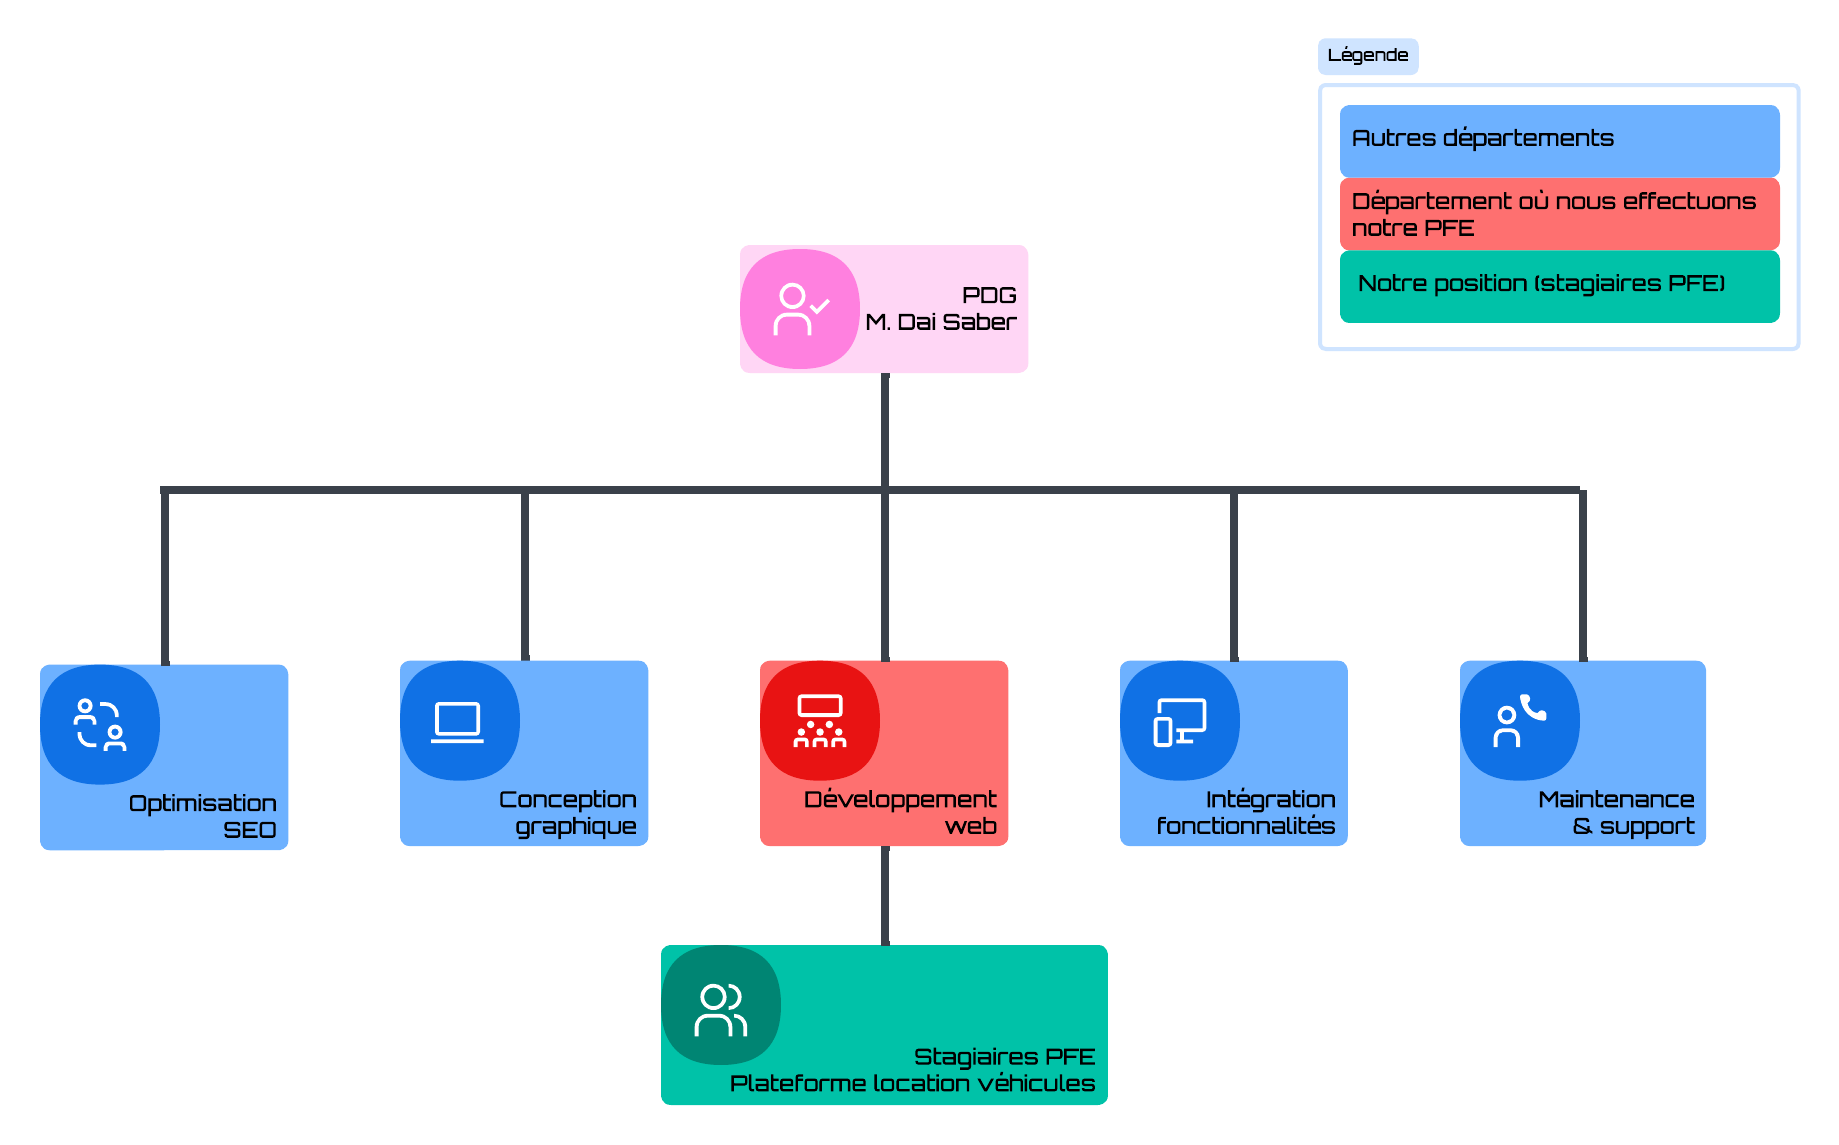
\includegraphics[width=1\textwidth]{Chapitres/Figures/organigramme.png}
    \caption{Organigramme de Yes Internet}
    \label{fig:organigramme}
\end{figure}

Dans le cadre de notre projet de fin d'études, nous sommes intégrés au sein du \textbf{départ-\\ement Développement Web}, sous la supervision directe du responsable 
technique. Notre mission consiste à concevoir et développer la plateforme intelligente 
de gestion de location de véhicules multi-agences.

%%%%%%%%%%%%%%%%%%%%%%%%%%%%%%%%%%%%%%%%%%%%%%%%%%%%%%%%%%%%%%%%%%%%%%%%%%
\section{Cadre et Présentation du Projet}
\label{sec:presentation}
%%%%%%%%%%%%%%%%%%%%%%%%%%%%%%%%%%%%%%%%%%%%%%%%%%%%%%%%%%%%%%%%%%%%%%%%
Dans le cadre de notre projet de fin d’études, l’entreprise \textbf{Yes Internet} nous a confié la réalisation d’un projet intitulé \textit{ Plateforme Intelligente de Gestion de Location de Véhicules Multi-Agences }. Ce projet constitue une opportunité de mobiliser et de mettre en application l’ensemble des connaissances théoriques et des compétences pratiques acquises tout au long de notre formation à l’École Supérieure d’Économie Numérique. Il s’inscrit également dans la perspective de l’obtention du diplôme de licence en informatique de gestion.
%%%%%%%%%%%%%%%%%%%%%%%%%%%%%%%%%%%%%%%%%%%%%%%%%%%%%%%%%%%%%%%%%%%%%%%%%%
\newpage
\section{Analyse de l'Existant}
\label{sec:existant}
%%%%%%%%%%%%%%%%%%%%%%%%%%%%%%%%%%%%%%%%%%%%%%%%%%%%%%%%%%%%%%%%%%%%%%%%%%
L'analyse de l'existant vise à enrichir l'étude des pistes innovantes 
d'un projet en cours de conception, avant sa mise en œuvre. Cette étude 
préalable permet de se faire une idée de la pertinence du projet, de sa 
faisabilité et de sa continuité.\cite{etude_faisabilite_cairn} 

\medskip

D'après notre analyse, le secteur de la gestion et suivie de location de véhicules dispose de plusieurs solutions à l'échelle internationale, mais les agences locales tunisiennes restent largement sous-équipées sur le plan numérique. Il devient donc crucial de réaliser une évaluation approfondie des systèmes actuels tant au niveau national qu'international.

%%%%%%%%%%%%%%%%%%%%%%%%%%%%%%%%%%%%%%%%%%%%%%%%%%%%%%%%%%%%%%%%%%%%%%%%%%
\subsection{Étude des solutions existantes au niveau national}
%%%%%%%%%%%%%%%%%%%%%%%%%%%%%%%%%%%%%%%%%%%%%%%%%%%%%%%%%%%%%%%%%%%%%%%%%%
Après avoir effectué des recherches liées aux applications numériques utilisées pour gérer le processus de location de véhicules en Tunisie, nous avons constaté que les pratiques adoptées par les agences locales varient en fonction des moyens et des outils disponibles.

Selon certaines études, le secteur de la location de voitures en Tunisie compte plusieurs centaines d’agences, ce qui témoigne de l’importance de cette activité et de la diversité des modes de gestion adoptés \cite{letemps_news}.

\begin{itemize}[noitemsep, topsep=0pt]
    \item \textbf{Processus de location et de réservation en Tunisie  :} \\Le client se rend directement à l’agence pour louer un véhicule. L’agent collecte les informations nécessaires, telles que les coordonnées du client, le type de véhicule souhaité, la durée de location et les documents requis (permis de conduire, carte d’identité, etc.). Le contrat de location est ensuite établi à partir de modèles standards utilisés dans le domaine \cite{scribd_contrat_standard}. Les informations relatives à la réservation, au contrat et à la disponibilité des véhicules sont consignées dans des supports internes tels que des registres ou des fichiers de suivi.


    \item \textbf{Suivi opérationnel et gestion de flotte :} \\Les agences utilisent des fiches de suivi ou des supports de pointage pour enregistrer les mouvements des véhicules (mise à disposition, retour, état du véhicule).


    \item \textbf{Contrats et gestion financière :} \\Les contrats de location, les paiements, les factures et les cautions sont enregistrés à l’aide des supports manuelles, fin de constituer un historique des opérations effectuées.  
     \\Exemple ci‑dessous :
    \\ \textit{Contrats de location papier} : Les agences utilisent fréquemment des formulaires papier pré-imprimés pour établir les contrats de location, nécessitant une saisie manuelle des informations client et véhicule, puis ces contrats sont archivés sous forme papier, servant à établir un historique des opérations de l’agence. 
        \\(Voir Figure \cite{modele-contrat-location-vehicule}).




    \item \textbf{Utilisation d’outils informatiques standards :}\\ Certaines agences s’appuient sur des outils tels que des tableurs pour organiser les réservations et suivre les informations liées aux clients et aux véhicules \cite{youtube_excel_gestion}.
    Exemple ci‑dessous :
    \\ \textit{Gestion de flotte via Excel} : Certaines agences utilisent des feuilles de calcul Excel pour gérer leur flotte, les réservations et la facturation, ce qui est sujet aux erreurs et manque d'automatisation. (Voir Figure \cite{gestion-de-location-par_excel}).
\end{itemize}
%%%%%%%%%%%%
\begin{figure}[H]
    \centering
    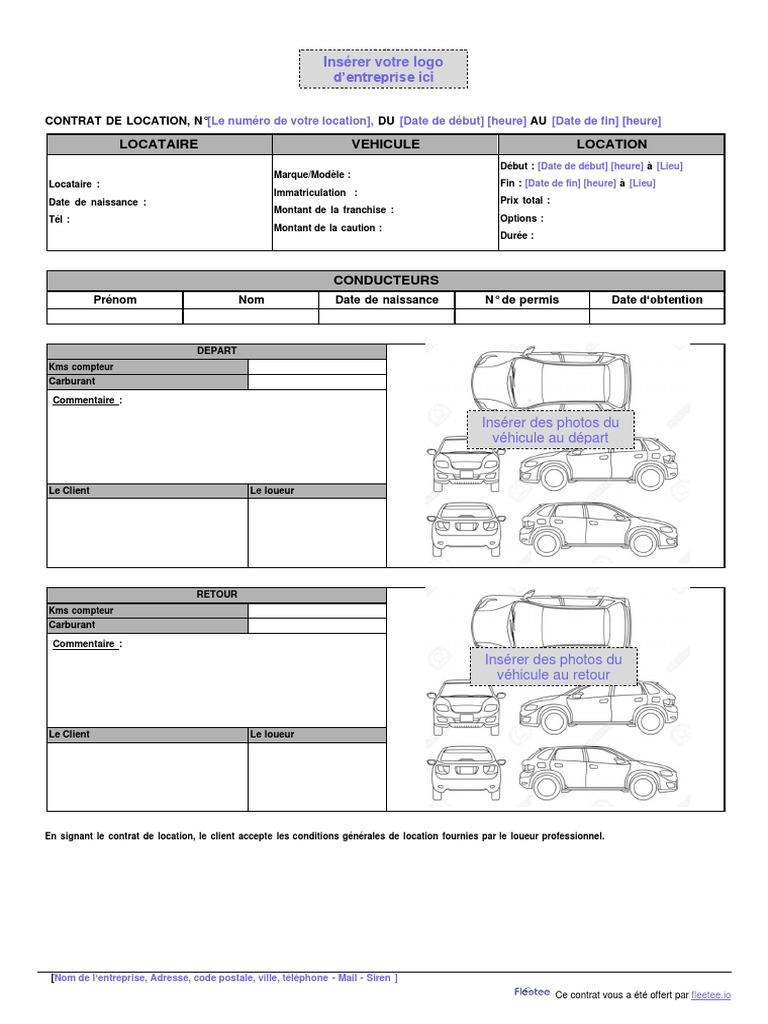
\includegraphics[width=0.8\textwidth]{Chapitres/Figures/contrat_papier.jpg}
    \caption{Modèle de contrat de location de véhicule. \cite{modele-contrat-location-vehicule} }
    \label{fig:contrat}
\end{figure}
%%%%%%%%%%%%
\begin{figure}[H]
    \centering
    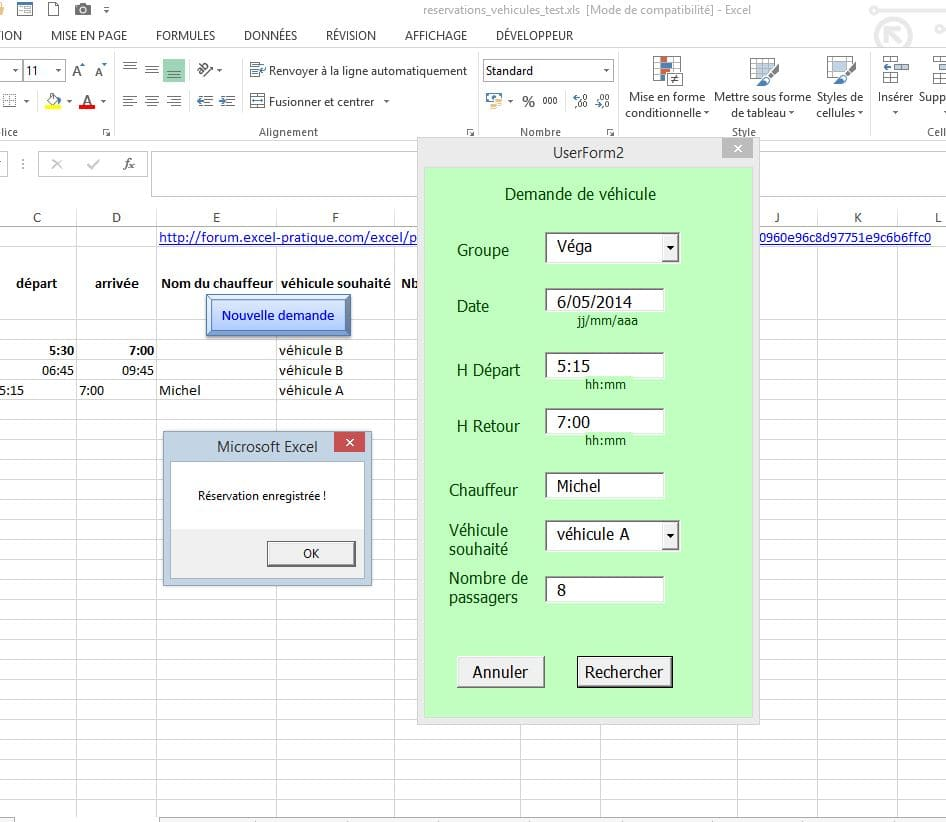
\includegraphics[width=1\textwidth]{Chapitres/Figures/gestion_excel.jpg}
    \caption{Gestion de locations des voitures par Excel.\cite{gestion-de-location-par_excel}}
    \label{fig:excel}
\end{figure}

\begin{itemize}[noitemsep, topsep=0pt]
    \item \textbf{Solutions numériques spécialisées pour la location :}\\
En parallèle, il existe des solutions numériques dédiées à la gestion de la location de véhicules. \textbf{Des logiciels spécialisés} proposent des fonctionnalités telles que la gestion des réservations, le suivi de la flotte automobile et la facturation \cite{renthub_tarifs}\cite{Logiciel_de_gestion_des_locations}. De même, certaines \textbf{plateformes en ligne} permettent de consulter les offres de location et d’effectuer des réservations à distance \cite{tunisiadrive_benefits}.
\end{itemize}
%%%%%%%%%%%%
\begin{figure}[H]
    \centering
    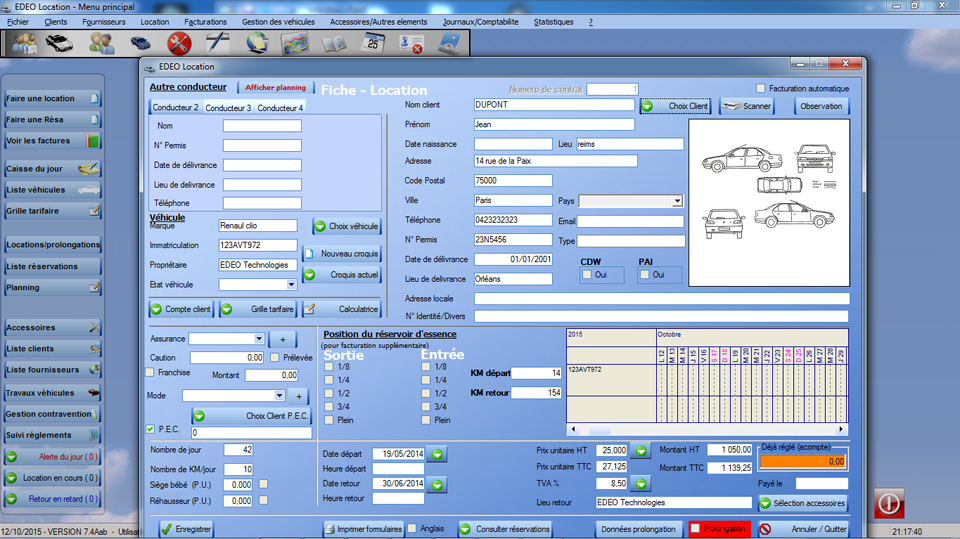
\includegraphics[width=0.9\textwidth]
    {Chapitres/Figures/exmp_sys.png}
    \caption{EDEO: Logiciel interne de gestion des locations.\cite{Logiciel_de_gestion_des_locations} }
    \label{fig:exmp_sys}
\end{figure}
%%%%%%%%%%%%%
\begin{figure}[H]
    \centering
    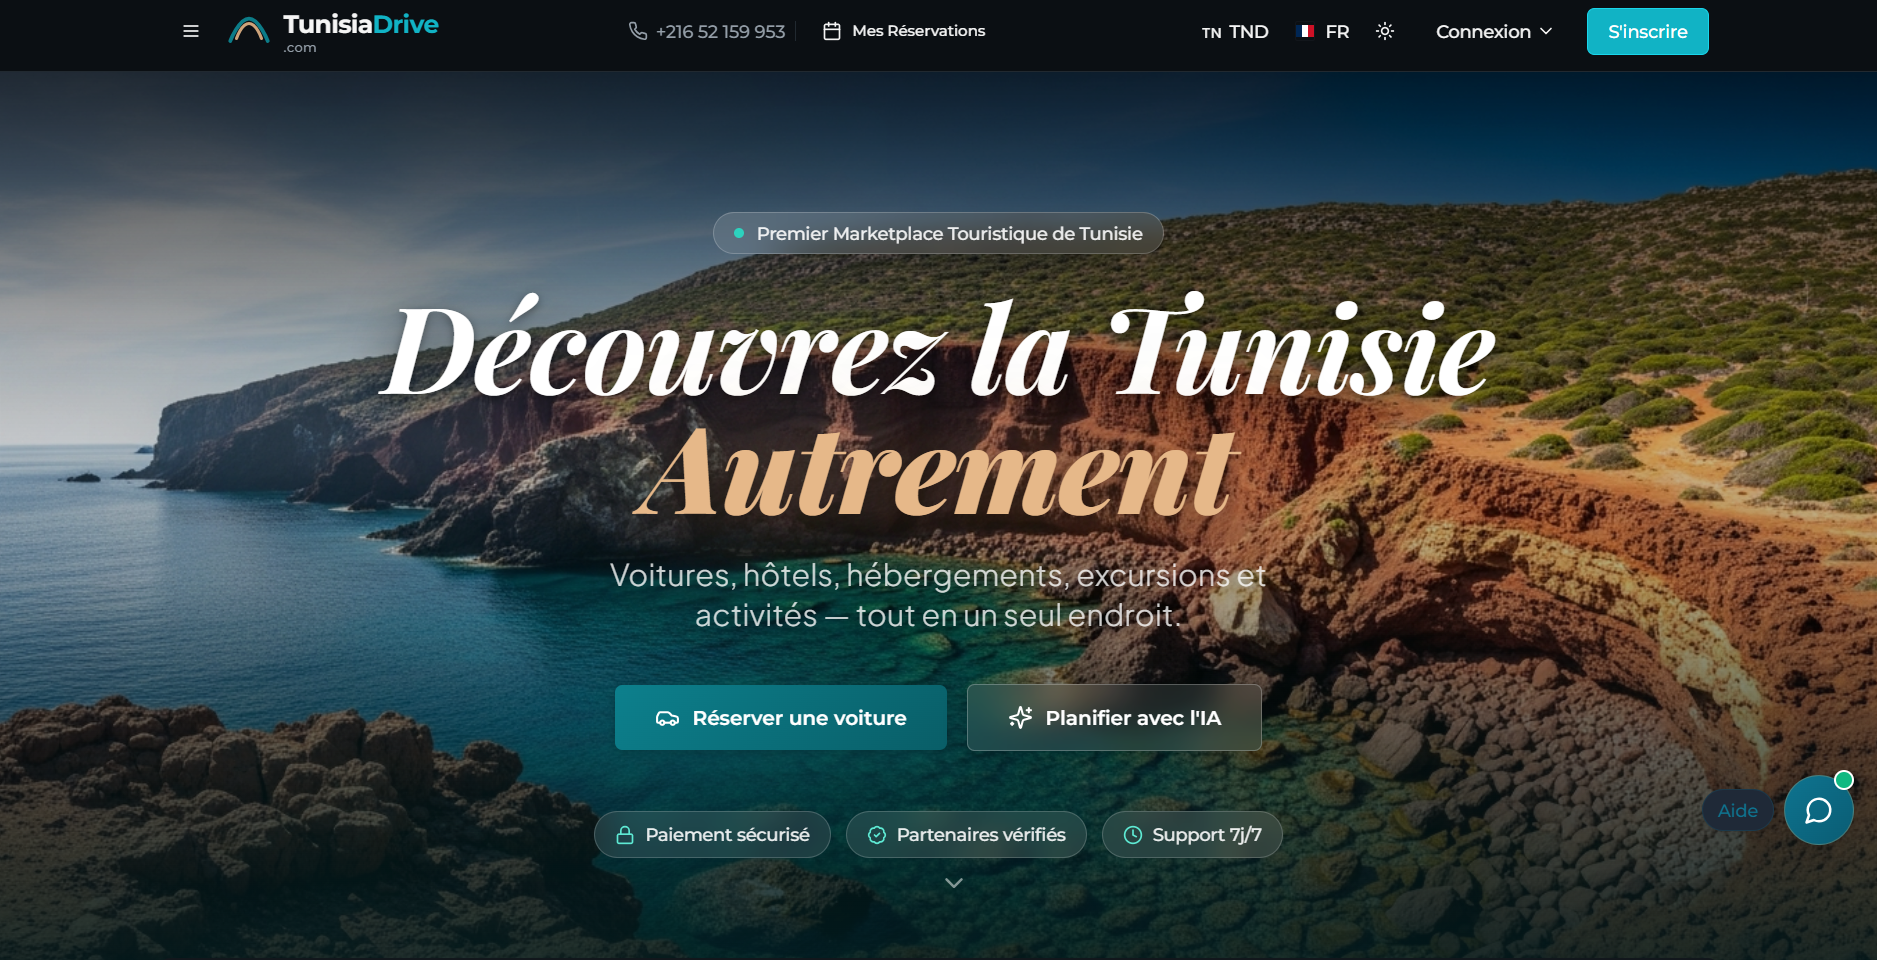
\includegraphics[width=0.9\textwidth]
    {Chapitres/Figures/tunisiadr.png}
    \caption{Plateforme de locations des voitures en Tunisie.\cite{tunisiadrive_benefits} }
    \label{fig:tunisiadrive}
\end{figure}
%%%%
Ainsi, ces observations montrent que les pratiques de gestion dans le domaine de la location de véhicules en Tunisie reposent sur une diversité de solutions, allant de l’utilisation de supports internes et d’outils génériques à l’intégration de solutions numériques dédiées au secteur.
%%%%

%%%%%%%%%%%%%%%%%%%%%%%%%%%%%%%%%%%%%%%%%%%%%%%%%%%%%%%%%%%%%%%%%%%%%%%%%%



\newpage
\subsection{Étude des solutions existantes au niveau international}
%%%%%%%%%%%%%%%%%%%%%%%%%%%%%%%%%%%%%%%%%%%%%%%%%%%%%%%%%%%%%%%%%%%%%%%%%%
Nous procédons ici à une analyse approfondie d'une solution de gestion de location des véhicules disponible à l'international, retenue pour sa représentativité, sa maturité et sa large adoption sur le marché mondial.
\subsubsection{Analyse de la plateforme Rent Centric}
Rent Centric est une plateforme cloud de référence dans le domaine de la gestion de location de véhicules, fondée en 2002 et utilisée par des centaines d'agences à travers le monde, notamment en Amérique du Nord, en Europe et au Moyen-Orient. Elle s'adresse aussi bien aux petites agences indépendantes qu'aux grandes entreprises multi-sites \cite{rc}.
\\La plateforme propose un ensemble de fonctionnalités permettant de couvrir l'intégralité du processus de location :
\begin{itemize}[noitemsep, topsep=0pt]
    \item \textbf{Réservation en ligne :} réservations en temps réel avec confirmation automatique et gestion des disponibilités.
    \item \textbf{Gestion de flotte :} suivi complet des véhicules, historique d'utilisation et planification de maintenance.
    \item \textbf{Gestion des contrats :} génération automatique des contrats, prolongations et gestion des retours.
    \item \textbf{Tarification dynamique :} grilles tarifaires configurables selon la saison, la durée et le profil client.
    \item \textbf{Gestion multi-agences :} administration centralisée avec tableaux de bord personnalisés par site.
    \item \textbf{Rapports et analytique :} rapports détaillés sur les performances et le taux d'occupation de la flotte.
\end{itemize}
\begin{figure}[H]
    \centering
    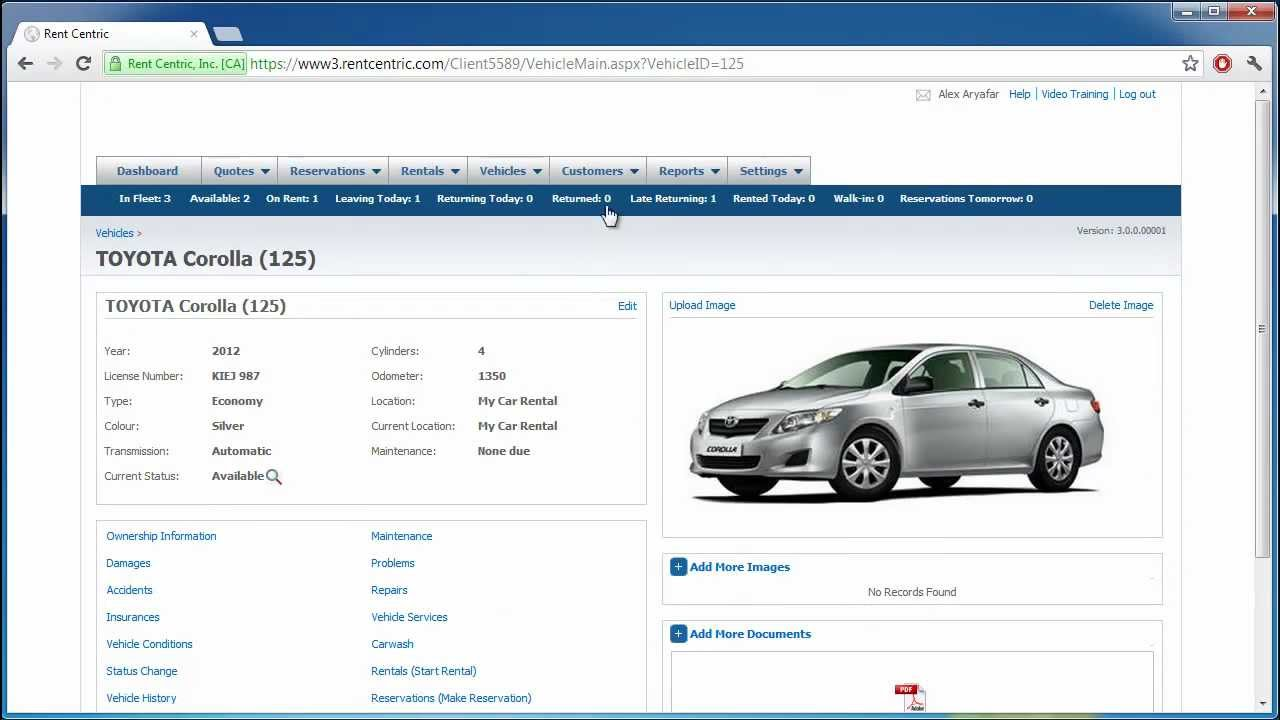
\includegraphics[width=0.85\textwidth]{Chapitres/Figures/car_centric.jpg}
    \caption{Aperçu des fonctionnalités de Rent Centric \cite{rc}}
    \label{fig:rent_centric}
\end{figure}

%%%%%%%%%%

\subsubsection{Analyse de HQ Rental Software}
HQ Rental Software est une solution complète de gestion de flotte de véhicules, conçue pour optimiser l'efficacité opérationnelle et améliorer l'expérience client. Elle offre une gamme étendue de fonctionnalités pour les entreprises de location de voitures de toutes tailles.\cite{hq_features}
\begin{itemize}[noitemsep, topsep=0pt]
    \item \textbf{Réservations et paiements en ligne :} Permet aux clients de réserver et de payer directement via un plugin de site web convivial, augmentant ainsi la portée du marché et améliorant l'expérience client.
    \item \textbf{Gestion de flotte :} Offre des outils pour gérer la disponibilité des véhicules, les réparations et les finances, réduisant la dépendance aux feuilles de calcul manuelles.
    \item \textbf{Dématérialisation :} Génère des contrats de location personnalisables qui peuvent être signés numériquement, avec la possibilité de télécharger des photos du véhicule via l'application mobile HQ.
    \item \textbf{Solutions pour divers marchés de location :} S'adapte à la location de motos, de bateaux, d'équipements et propose des solutions pour la location à long terme et le leasing.
    \item \textbf{Rapports avancés :} Fournit des tableaux de bord personnalisés pour suivre les indicateurs de performance clés et exporter les données nécessaires.
    \item \textbf{Paiements intégrés et comptabilité :} Automatise le processus de vente et la gestion des transactions financières.
    \item \textbf{Solution basée sur le cloud et accès mobile :} Accessible depuis n'importe quel appareil et n'importe où dans le monde, avec des applications Android et iOS dédiées.
\end{itemize}
\begin{figure}[H]
    \centering
    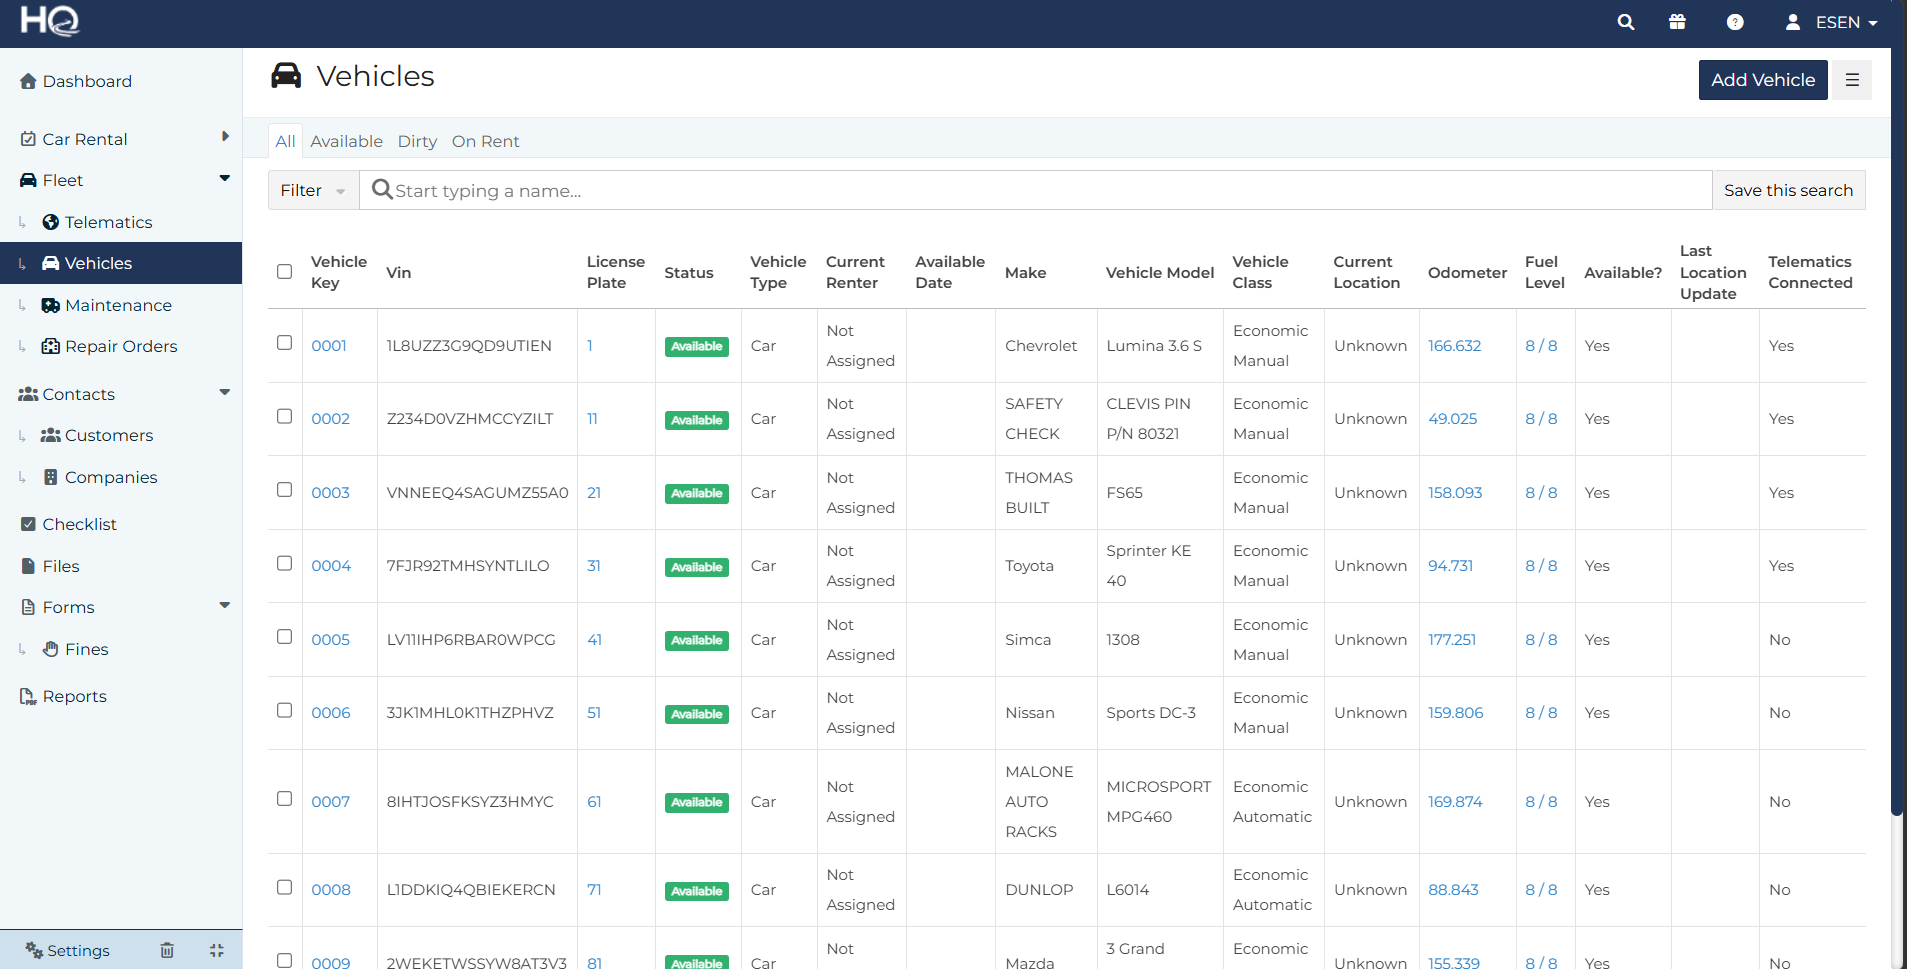
\includegraphics[width=0.85\textwidth]{Chapitres/Figures/HQ.png}
    \caption{Tableau de bord de HQ Rental Software. \cite{hq_features}}
    \label{fig:hq_dashboard}
\end{figure}

%%%%%%%%%%%%%%%%%%%%%%%%

\subsubsection{Analyse de VEVS Car Rental platform}
VEVS Car Rental Software est une solution logicielle et de site web intégrée pour les entreprises de location de voitures, visant à automatiser les processus, à rationaliser la gestion et à augmenter l'efficacité opérationnelle.\cite{vevs_features}
\begin{itemize}[noitemsep, topsep=0pt]
    \item \textbf{Réservations en ligne :} Permet aux clients de réserver des véhicules en ligne, avec des confirmations par e-mail automatiques et une page « My Booking » pour le suivi des réservations.
    \item \textbf{Gestion de flotte :} Outils pour gérer la disponibilité des véhicules, les réparations et les finances.
    \item \textbf{Tarification flexible et taxes configurables :} Permet de définir des options de tarification flexibles basées sur la durée de location et la demande, et de configurer les taxes (TVA, taxes touristiques, etc.).
    \item \textbf{Vente additionnelle d'extras et codes promotionnels :} Génère des revenus supplémentaires en proposant des extras (GPS, sièges enfant) et en créant des codes promotionnels pour les campagnes marketing.
    \item \textbf{Tarifs saisonniers et autres frais :} Permet de générer des structures de prix saisonnières distinctives et d'ajouter des frais supplémentaires (relais, jeunes conducteurs, kilométrage supplémentaire).
    \item \textbf{Solution basée sur le cloud et accès mobile :} Permet de gérer l'entreprise depuis n'importe quel appareil et n'importe où dans le monde.
\end{itemize}
\begin{figure}[H]
    \centering
    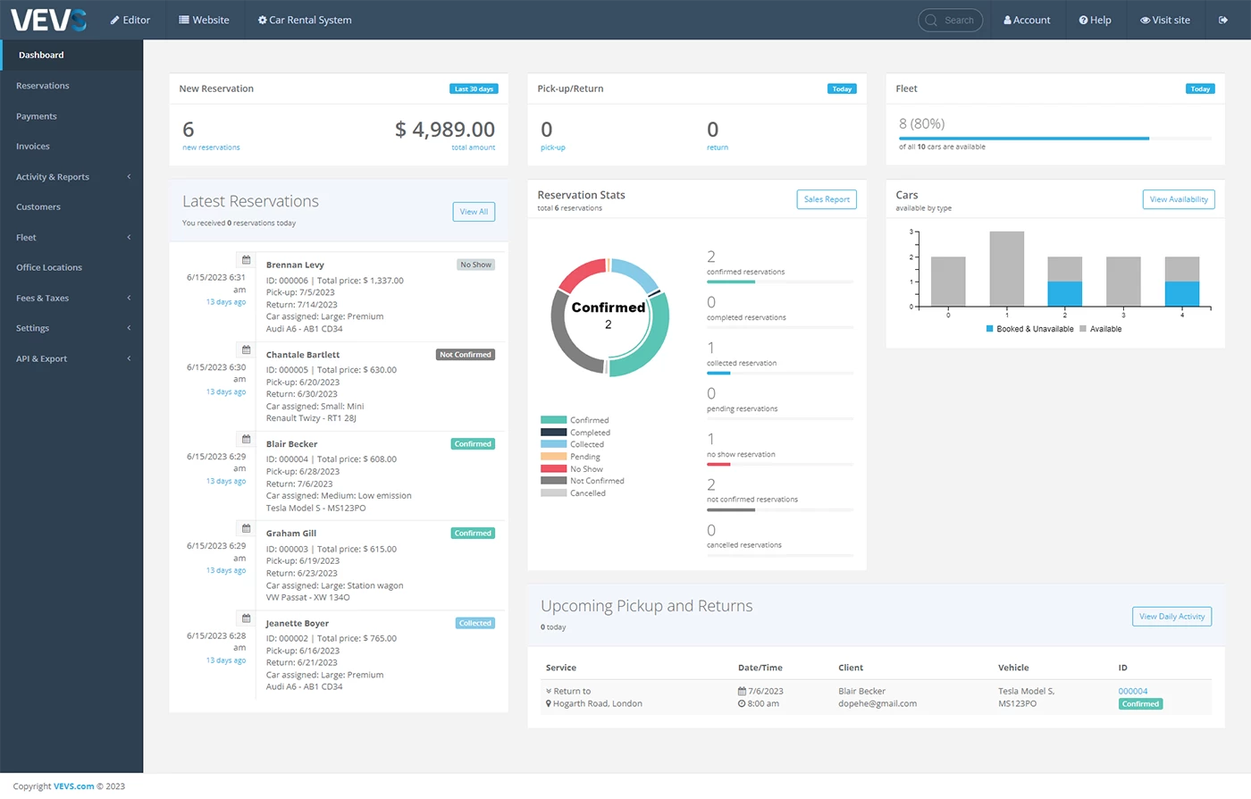
\includegraphics[width=0.8\textwidth]{Chapitres/Figures/vevs_dashboard.png}
    \caption{Tableau de bord de VEVS Car Rental platform. \cite{vevs_features}}
    \label{fig:vevs_dashboard}
\end{figure}
%%%%%%%%%%%%%%%%%%%%%%%%%%%%%%%%%%%%%%%%%%%%%%%%%%%%%%%%%%%%%%%%%%%%%%%%%%
Cette analyse nous a permis d'identifier les fonctionnalités clés à intégrer dans notre solution, tout en ciblant les lacunes auxquelles notre projet se propose de répondre.
%%%%%%%%%%%%%%%%%%%%%%%%%%%%%%%%%%%%%%%%%%%%%%%%%%%%%%%%%%%%%%%%%%%%%%%%%%
\section{Critique de l'Existant}
\label{sec:critique}
\medskip
\medskip
%%%%%%%%%%%%%%%%%%%%%%%%%%%%%%%%%%%%%%%%%%%%%%%%%%%%%%%%%%%%%%%%%%%%%%%%%%
L'analyse du marché actuel révèle plusieurs insuffisances notables, résumées ci-dessous :
\medskip

\subsection{Critique des solutions existantes au niveau national}
\medskip
\medskip
\begin{itemize}[noitemsep, topsep=0pt]
    \item \textbf{Fragmentation du secteur} : Selon une étude récente, la Tunisie compte plus de 700 sociétés de location de voitures, ce qui traduit un marché fortement fragmenté et peu structuré. Cette dispersion complique la mise en place de solutions centralisées et favorise des pratiques hétérogènes entre les agences \cite{letemps_news}.
    \item \textbf{Faible digitalisation des agences} : Malgré l’existence de plateformes d’information et de réservation en ligne, plusieurs agences continuent d’utiliser des outils traditionnels (Excel, registres papier). Cela limite l’automatisation des processus et engendre une perte d’efficacité opérationnelle \cite{drivotunisie}.
    \item \textbf{Absence de plateformes unifiées} : Contrairement à d’autres marchés, il existe peu de plateformes nationales intégrées permettant de centraliser les offres de plusieurs agences. Les solutions existantes sont souvent limitées à des vitrines ou à des sites informatifs sans réelle interconnexion des données.
    \item \textbf{Manque de visibilité globale} : Les plateformes locales disponibles ne proposent généralement pas de tableaux de bord analytiques avancés. Cela empêche les agences de suivre en temps réel leurs performances ou d’exploiter les données pour optimiser leur activité.
    \item \textbf{Expérience utilisateur limitée} : Les systèmes actuels offrent une expérience client fragmentée (réservation, paiement, suivi). L’absence d’intégration complète (réservation en ligne, paiement sécurisé, suivi du véhicule) réduit l’attractivité des services proposés.
    \item \textbf{Difficulté d’adaptation technologique} : Les agences rencontrent des difficultés à intégrer des technologies modernes (paiement en ligne, géolocalisation, gestion automatisée). Cela est dû au manque de solutions locales adaptées et au coût des alternatives internationales.
\end{itemize}

\newpage
\subsection{Critique des solutions existantes au niveau international}
\medskip
\medskip
\medskip
\begin{itemize}[noitemsep, topsep=0pt]
    \item \textbf{Coût élevé et accessibilité limitée} : Les plateformes et logiciels internationaux de gestion de location (SaaS: Software as a Service) impliquent des coûts d’abonnement élevés, ce qui constitue une barrière importante pour les petites et moyennes agences tunisiennes.
    \item \textbf{Complexité d’intégration} : Ces solutions nécessitent souvent une intégration technique complexe (API, configuration avancée), difficile à mettre en œuvre dans des environnements locaux disposant de ressources techniques limitées.
    \item \textbf{Orientation SaaS plutôt que plateforme} : La majorité des solutions internationales sont conçues comme des outils de gestion interne (SaaS) et non comme des plateformes collaboratives multi-agences. Elles ne favorisent donc pas la mutualisation des offres ni la visibilité globale du marché.
    \item \textbf{Manque d’adaptation au contexte local} : Ces solutions ne prennent pas en compte les spécificités tunisiennes (réglementation, fiscalité, modes de paiement locaux). Leur utilisation nécessite souvent des adaptations coûteuses et complexes.
    \item \textbf{Fonctionnalités surdimensionnées} : Certaines plateformes proposent des fonctionnalités avancées (ERP complets) qui dépassent les besoins réels des agences locales, entraînant une complexité inutile et une faible adoption.
    \item \textbf{Dépendance au fournisseur} : L’utilisation de solutions SaaS implique une dépendance forte vis-à-vis du fournisseur (hébergement, sécurité, mises à jour), ce qui peut poser des risques en cas d’interruption du.\cite{journaldunet}
    \item \textbf{Expérience utilisateur non localisée} : Même si certaines plateformes sont multilingues, elles ne sont pas toujours adaptées au contexte culturel et linguistique tunisien, ce qui peut nuire à leur adoption par les utilisateurs locaux.
    \item \textbf{Absence de logique marketplace locale} : Contrairement à des plateformes globales comme les marketplaces internationales, les solutions existantes ne permettent pas de fédérer plusieurs agences tunisiennes au sein d’un écosystème numérique commun.
\end{itemize}
%%%%%%%%%%%%%%%%%%%%%%%%%%%%%%%%%%%%%%%%%%%%%%%%%%%%%%%%%%%%%%%%%%%%%%%%%%
\newpage
\section{Solution Proposée}
\label{sec:solution}
%%%%%%%%%%%%%%%%%%%%%%%%%%%%%%%%%%%%%%%%%%%%%%%%%%%%%%%%%%%%%%%%%%%%%%%%%%

Pour remédier aux limites identifiées dans l'analyse du marché actuel, nous proposons le développement d'une plateforme web intelligente de gestion de location de véhicules multi-agences, entièrement adaptée au contexte tunisien. Notre solution présentera plusieurs avantages distinctifs :

\begin{itemize}[noitemsep, topsep=0pt]
    \item \textbf{Une architecture multi-agences centralisée} permettant de gérer l'ensemble du système depuis une interface unique
    \item \textbf{Une gestion complète du processus de location} (véhicule disponible, réservé, en cours d'utilisation, retourné ou en maintenance)
    \item \textbf{Une expérience utilisateur intégrée} couvrant l’ensemble du processus de location (recherche, réservation, paiement et suivi) via une interface intuitive et ergonomique
    \item \textbf{Un système de sécurité renforcé} assurant l’authentification des utilisateurs, la gestion des accès et la protection des données sensibles
    \item \textbf{Un système de paiement en ligne sécurisé} permettant aux clients d’effectuer leurs transactions directement via la plateforme
    \item \textbf{Une gestion automatisée des contrats de location} incluant leur génération, leur archivage et leur consultation
    \item \textbf{Un suivi du statut des réservations} avec un historique complet par agence et par client
    \item \textbf{Un système de score de fiabilité client} calculé automatiquement selon le comportement historique de chaque client (retards, annulations, incidents)
    \item \textbf{Des tableaux de bord analytiques} offrant une visibilité complète sur les indicateurs clés de performance
    \item \textbf{Une architecture ouverte} basée sur des API facilitant l’intégration avec des systèmes externes
    \item \textbf{Une adaptation aux spécificités du contexte tunisien}, notamment en termes de réglementation et modes de paiement locaux
    \item \textbf{Une solution accessible et adaptée aux petites et moyennes agences} grâce à une conception optimisée et des coûts réduits
    \item \textbf{Une interface simple et facile à prendre en main} favorisant une adoption rapide par les agences
    \item \textbf{Une architecture modulaire et évolutive} basée sur des technologies modernes garantissant performance et maintenabilité
    \item \textbf{Une architecture scalable} capable de supporter un grand nombre d’agences et d’utilisateurs simultanément
\end{itemize}

Enfin, notre plateforme sera conçue en s'inspirant des meilleures pratiques des solutions analysées, tout en restant adaptée aux besoins et contraintes du marché tunisien.

%%%%%%%%%%%%%%%%%%%%%%%%%%%%%%%%%%%%%%%%%%%%%%%%%%%%%%%%%%%%%%%%%%%%%%%%%%
\section{Méthodologie et Modélisations}
\label{sec:methodo}
%%%%%%%%%%%%%%%%%%%%%%%%%%%%%%%%%%%%%%%%%%%%%%%%%%%%%%%%%%%%%%%%%%%%%%%%%%

L'implémentation de stratégies de gestion performantes est l'une des clés de la réussite d'un projet et d'une bonne coordination entre les différentes phases. Cela implique le déploiement d'une bonne méthodologie de gestion de projet et de langages de modélisation 
adaptés.

%%%%%%%%%%%%%%%%%%%%%%%%%%%%%%%%%%%%%%%%%%%%%%%%%%%%%%%%%%%%%%%%%%%%%%%%%%
\subsection{Les méthodes agiles}
%%%%%%%%%%%%%%%%%%%%%%%%%%%%%%%%%%%%%%%%%%%%%%%%%%%%%%%%%%%%%%%%%%%%%%%%%%

La méthode Agile se base sur un cycle de développement itératif qui place le client au centre du processus \cite{atlassian}. Contrairement aux méthodes classiques qui suivent une approche linéaire et séquentielle avec des spécifications figées dès le départ, les méthodes agiles privilégient la flexibilité, la collaboration et la livraison fréquente de versions 
fonctionnelles. Grâce à cette approche, le demandeur obtient une meilleure visibilité sur la gestion des travaux, et l'équipe bénéficie d'un feedback régulier pour appliquer directement les changements nécessaires.Les données présentées dans le Tableau \ref{tab:agile_vs_classique} illustrent les 
principales différences entre les méthodes classiques et les méthodes agiles.

\begin{table}[H]
\centering
\caption{Tableau comparatif entre méthodes classiques et méthodes agiles}
\label{tab:agile_vs_classique}
\begin{tabular}{|p{7cm}|p{7cm}|}
\hline
\textbf{Méthode classique} & \textbf{Méthode agile} \\
\hline
Approche linéaire et séquentielle & Approche itérative et incrémentale \\
\hline
Moins de flexibilité & Très flexible et adaptable \\
\hline
Une seule livraison à la fin du projet & Des livraisons fréquentes et régulières \\
\hline
\end{tabular}
\end{table}
\FloatBarrier
\begin{figure}[H]
    \centering
    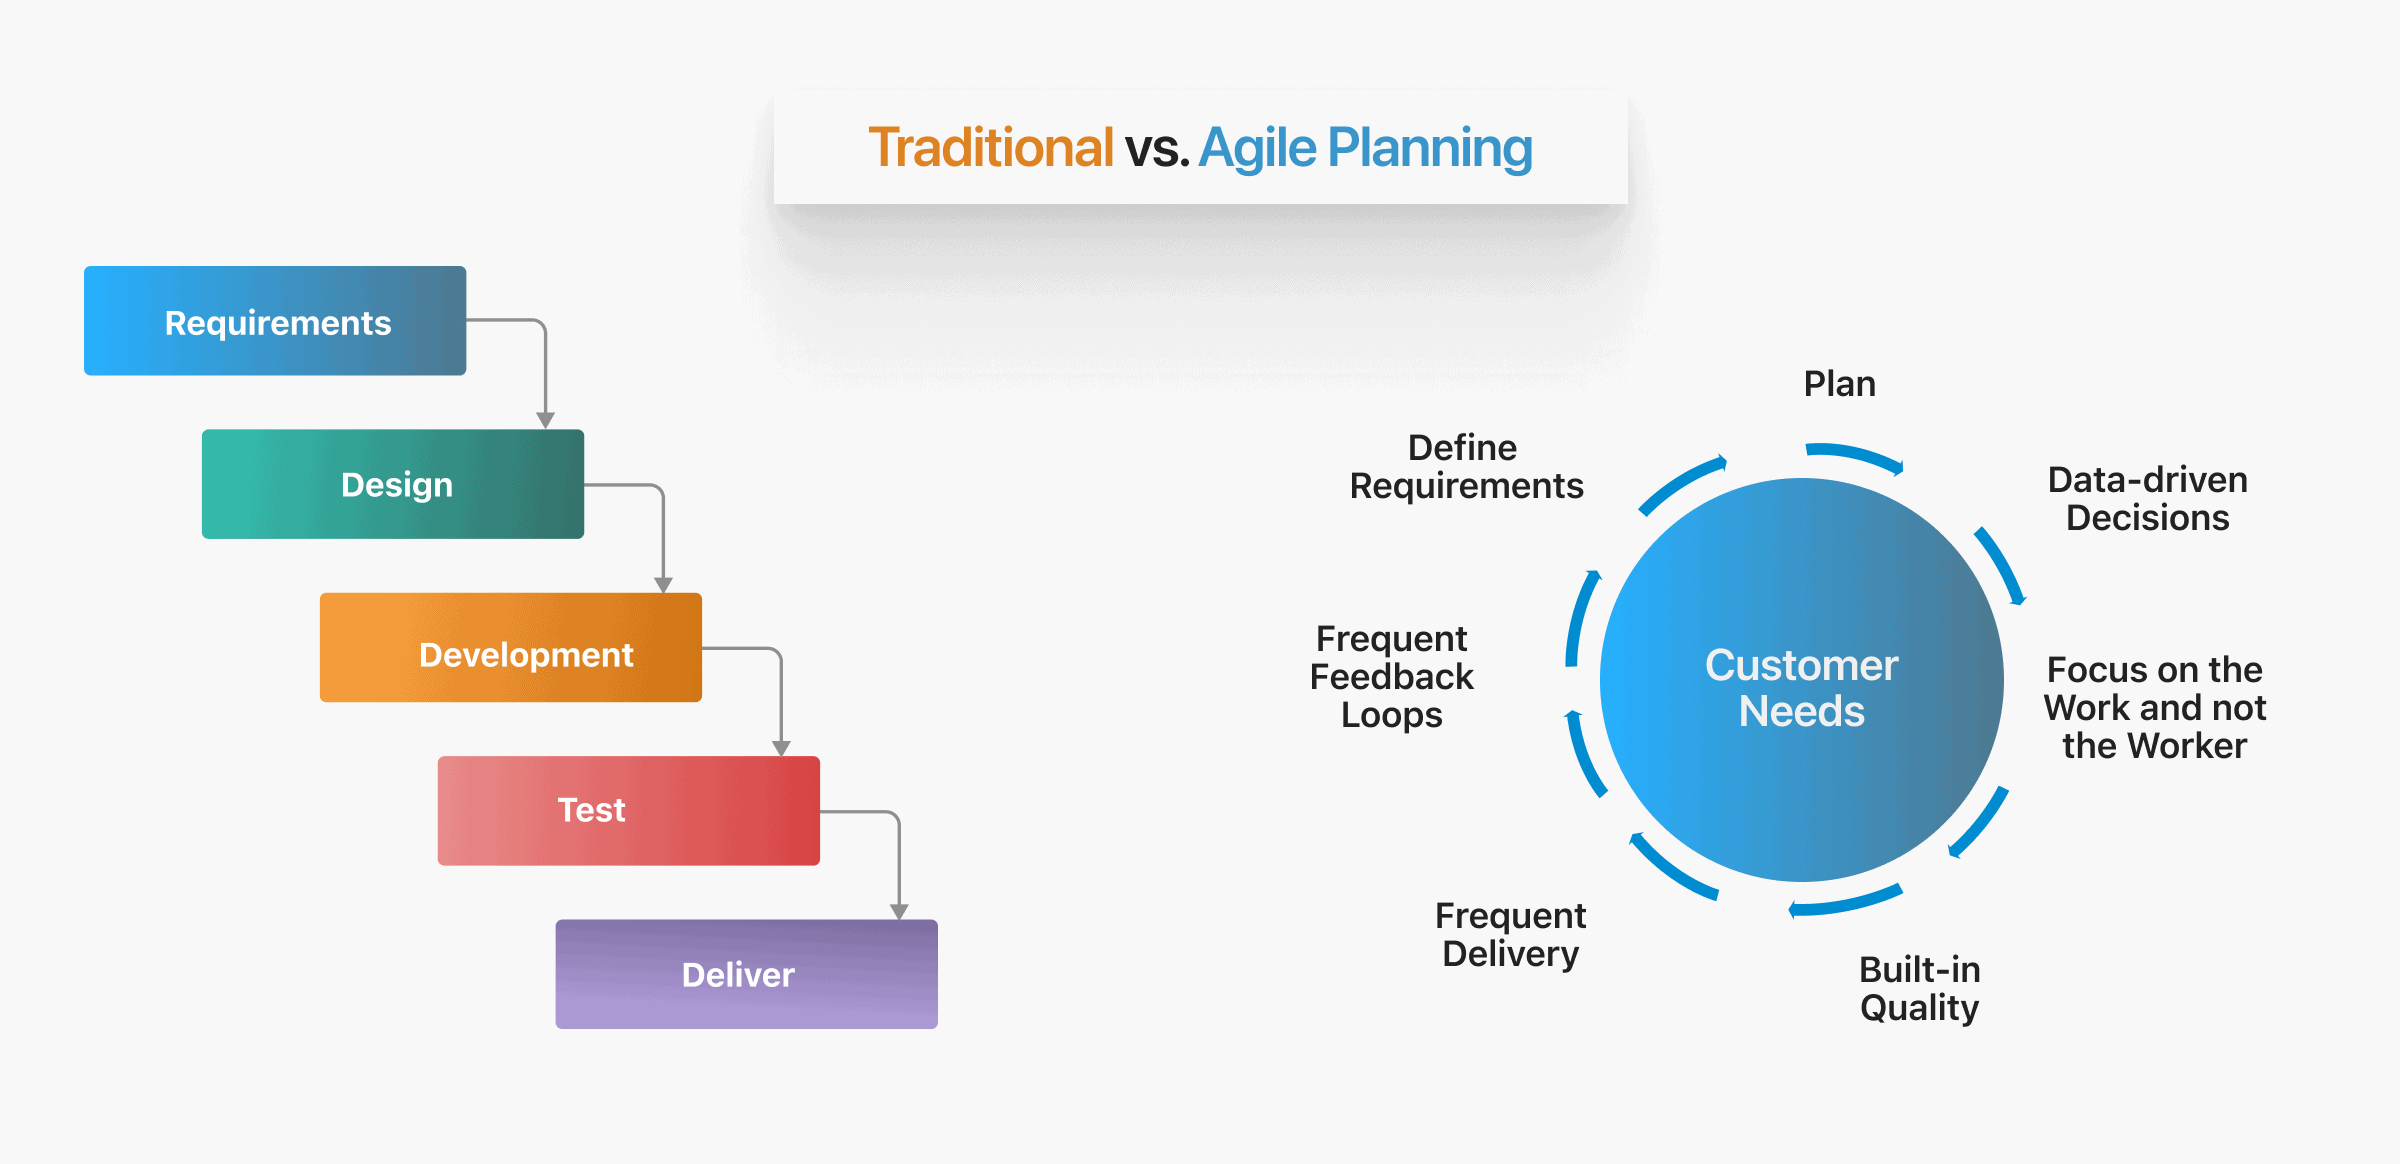
\includegraphics[width=0.9\textwidth]{Chapitres/Figures/agile.png}
    \caption{Agile vs approches classiques}
    \label{fig:agile}
\end{figure}

Parmi les méthodes agiles les plus reconnues dans le domaine du génie logiciel, on trouve 
Scrum, Kanban, Extreme Programming (XP), SAFe et Crystal. En vue de mener notre projet 
de manière efficace et de fournir un produit de qualité dans les délais impartis, nous 
avons opté pour la méthodologie \textbf{Scrum}.

%%%%%%%%%%%%%%%%%%%%%%%%%%%%%%%%%%%%%%%%%%%%%%%%%%%%%%%%%%%%%%%%%%%%%%%%%%
\subsection{La méthodologie Scrum}
%%%%%%%%%%%%%%%%%%%%%%%%%%%%%%%%%%%%%%%%%%%%%%%%%%%%%%%%%%%%%%%%%%%%%%%%%%

 \textit{"SCRUM est un cadre de travail dans lequel les personnes peuvent aborder des problèmes complexes et adaptatifs tout en livrant de manière efficace et créative des produits de la plus grande valeur possible.''} \cite{scrum}


Il s'agit d'une approche itérative et progressive qui évite l'effet \og tunnel \fg{}, où 
les résultats ne sont visibles qu'à la clôture du projet. C'est également une approche 
collaborative dans laquelle tous les membres de l'équipe sont actifs et contribuent aux 
décisions. Scrum s'articule autour de trois acteurs principaux :

\begin{itemize}[noitemsep, topsep=0pt]
    \item \textbf{Product Owner :} Il détient la responsabilité du produit ; c'est le client 
    qui communique ses attentes et approuve le travail lors des revues de sprint.
    \item \textbf{Scrum Master :} Il supervise le bon déroulement de la mission et résout 
    les obstacles qui entravent l'avancement du projet.
    \item \textbf{Scrum Team :} Ensemble d'individus en charge d'exécuter les exigences, 
    incluant développeurs, concepteurs et testeurs.
\end{itemize}

\begin{figure}[H]
    \centering
    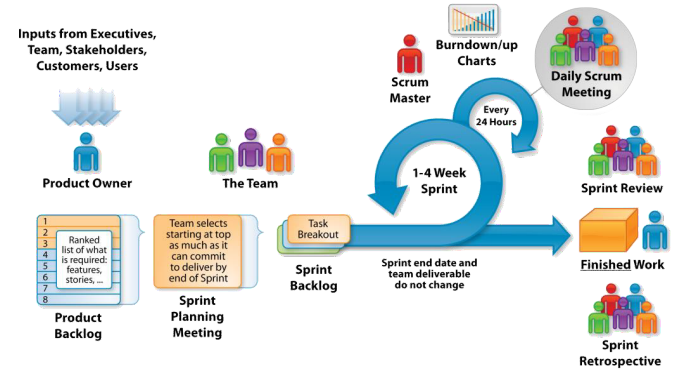
\includegraphics[width=0.7\textwidth]{Chapitres/Figures/scrum_model.png}
    \caption{Les caractéristiques du modèle Scrum}
    \label{fig:scrum_model}
\end{figure}

%%%%%%%%%%%%%%%%%%%%%%%%%%%%%%%%%%%%%%%%%%%%%%%%%%%%%%%%%%%%%%%%%%%%%%%%%%
\subsection{Product Backlog et Sprint Backlog}
%%%%%%%%%%%%%%%%%%%%%%%%%%%%%%%%%%%%%%%%%%%%%%%%%%%%%%%%%%%%%%%%%%%%%%%%%%

Dans la méthodologie Scrum, deux artefacts essentiels structurent la gestion des tâches 
et des priorités tout au long du projet.

Le \textbf{Product Backlog} est une liste ordonnée et exhaustive de toutes les 
fonctionnalités, exigences et améliorations souhaitées pour le produit final. Il est 
géré et priorisé par le Product Owner selon la valeur métier de chaque élément. Il 
évolue continuellement tout au long du projet en fonction des retours des parties prenantes 
et des besoins émergents. Chaque élément du Product Backlog est exprimé sous forme de 
\textbf{User Stories}, décrivant une fonctionnalité du point de vue de l'utilisateur.

Le \textbf{Sprint Backlog}, quant à lui, représente la sélection des User Stories issues 
du Product Backlog que l'équipe s'engage à réaliser durant un sprint donné. Contrairement 
au Product Backlog qui couvre l'ensemble du projet, le Sprint Backlog est limité à une 
itération précise (2 à 4 semaines) et appartient à l'équipe de développement. Il est 
défini lors du Sprint Planning et ne doit pas être modifié en cours de sprint.

\begin{table}[H]
\centering
\caption{Différence entre Product Backlog et Sprint Backlog}
\label{tab:backlogs}
\begin{tabular}{|p{3.5cm}|p{5cm}|p{5cm}|}
\hline
\textbf{Critère} & \textbf{Product Backlog} & \textbf{Sprint Backlog} \\
\hline
Portée & Ensemble du projet & Un seul sprint \\
\hline
Propriétaire & Product Owner & Équipe de développement \\
\hline
Contenu & Toutes les User Stories & User Stories sélectionnées \\
\hline
Évolution & Continu et dynamique & Figé pendant le sprint \\
\hline
Priorité & Définie par valeur métier & Définie par le Sprint Planning \\
\hline
\end{tabular}
\end{table}

%%%%%%%%%%%%%%%%%%%%%%%%%%%%%%%%%%%%%%%%%%%%%%%%%%%%%%%%%%%%%%%%%%%%%%%%%%
\section{Langage de Modélisation : UML}
\label{sec:uml}
%%%%%%%%%%%%%%%%%%%%%%%%%%%%%%%%%%%%%%%%%%%%%%%%%%%%%%%%%%%%%%%%%%%%%%%%%%

Pour la conception de notre système, nous avons adopté l'\textbf{UML} (Unified Modeling 
Language), un langage graphique composé de diagrammes offrant différentes 
perspectives sur le système en cours de réalisation.

\begin{figure}[H]
    \centering
    
\includegraphics[width=0.2\textwidth]{Chapitres/Figures/UML-logo.png}
    \caption{Logo UML}
    \label{fig:uml_logo}
\end{figure}

L'UML est un standard reconnu internationalement qui présente plusieurs atouts : il est 
sans ambiguïtés, universel, adaptable à tout langage orienté objet, et facilite la 
communication entre les membres de l'équipe et les parties prenantes. Dans le cadre de 
notre projet, nous utiliserons principalement le \textbf{diagramme de cas d'utilisation} 
pour modéliser les interactions entre les acteurs et le système, ainsi que le 
\textbf{diagramme de séquence} pour décrire le déroulement des scénarios fonctionnels.\cite{uml}

%%%%%%%%%%%%%%%%%%%%%%%%%%%%%%%%%%%%%%%%%%%%%%%%%%%%%%%%%%%%%%%%%%%%%%%%%%
\section{Conclusion}
%%%%%%%%%%%%%%%%%%%%%%%%%%%%%%%%%%%%%%%%%%%%%%%%%%%%%%%%%%%%%%%%%%%%%%%%%%

Dans ce premier chapitre, nous avons présenté notre organisme d'accueil Yes Internet ainsi que le cadre général du projet. Nous avons analysé les solutions existantes au niveau national et international, résumé leurs lacunes, et proposé notre solution adaptée au contexte tunisien. 

\medskip

Enfin, nous avons présenté la méthodologie de gestion de projet utilisée ainsi que le langage de modélisation qui guideront la conduite du projet.

\medskip

Dans le chapitre qui suit, nous aborderons la planification de notre projet.
%%%%%%%%%%%%%%%%%%%%%%%%%%%%%%%%%%%%%%%%%%%%%%%%%%%%%%%%%%%%%%%%%%%%%%%%%
\chapter{Planification et architecture}
\label{Chapitre_2}
%%%%%%%%%%%%%%%%%%%%%%%%%%%%%%%%%%%%%%%%%%%%%%%%%%%%%%%%%%%%%%%%%%%%%%%%%%%
\section*{Introduction}
%%%%%%%%%%%%%%%%%%%%%%%%%%%%%%%%%%%%%%%%%%%%%%%%%%%%%%%%%%%%%%%%%%%%%%%%%%%

La planification constitue une étape essentielle dans la mise en œuvre d'un projet. Ainsi, dans ce chapitre, nous allons identifier et analyser \textbf{les différentes parties prenantes} du système. \\Ensuite, nous présenterons \textbf{les besoins fonctionnels} et \textbf{non fonctionnels}, \textbf{les diagrammes de cas d'utilisation}, ainsi que l'organisation du projet en \textbf{sprints} Scrum.
%%%%%%%%%%%%%%%%%%%%%%%%%%%%%%%%%%%%%%%%%%%%%%%%%%%%%%%%%%%%%%%%%%%%%%%%%%%
\section{Identification des acteurs}
\label{section2.1}
%%%%%%%%%%%%%%%%%%%%%%%%%%%%%%%%%%%%%%%%%%%%%%%%%%%%%%%%%%%%%%%%%%%%%%%%%%%

Notre application web implique cinq acteurs principaux :

\begin{itemize}
    \item \textbf{Internaute :} L'internaute peut consulter les actualités, intéragir avec un Chatbot et créer un 
    compte sur la plateforme pour accéder aux système.

    \item \textbf{Utilisateur :} L'utilisateur, qui peut être un client, une agence ou 
    un administrateur, a la possibilité de gérer son profil, consulter les offres et 
    voir son score client, après authentification.

    \item \textbf{Client :} Le client est un utilisateur souhaitant louer un 
    véhicule auprès d'une agence digitale .Suite à l’authentification, il peut consulter ses réservations en cours, 
    contacter une agence et voir son score de fiabilité.

    \item \textbf{Agence :} L'agence est une entreprise de location de véhicules utilisant 
    la plateforme pour gérer son activité.Dès son authentification, elle peut créer et gérer sa vitrine automobile, 
    suivre les réservations et les réclamations, valider ou refuser des demandes et accéder 
    aux statistiques.

    \item \textbf{Administrateur :}Une fois authentifié, l'administrateur supervise l'ensemble de la plateforme 
    pour garantir son bon fonctionnement. Il peut gérer les agences et les utilisateurs, 
    superviser les véhicules, consulter les KPI, détecter les anomalies et configurer les 
    paramètres système.
\end{itemize}

%%%%%%%%%%%%%%%%%%%%%%%%%%%%%%%%%%%%%%%%%%%%%%%%%%%%%%%%%%%%%%%%%%%%%%%%%%%
\section{Diagramme de contexte statique}
\label{section2.2}
%%%%%%%%%%%%%%%%%%%%%%%%%%%%%%%%%%%%%%%%%%%%%%%%%%%%%%%%%%%%%%%%%%%%%%%%%%%

Le diagramme de contexte statique permet de mettre en évidence les interactions 
au sein des différentes entités impliquées dans le système, tout en précisant le 
nombre d'exemplaires existant pour chaque intervenant connecté à un instant donné.\cite{ittrip}

\begin{figure}[H]
    \centering
    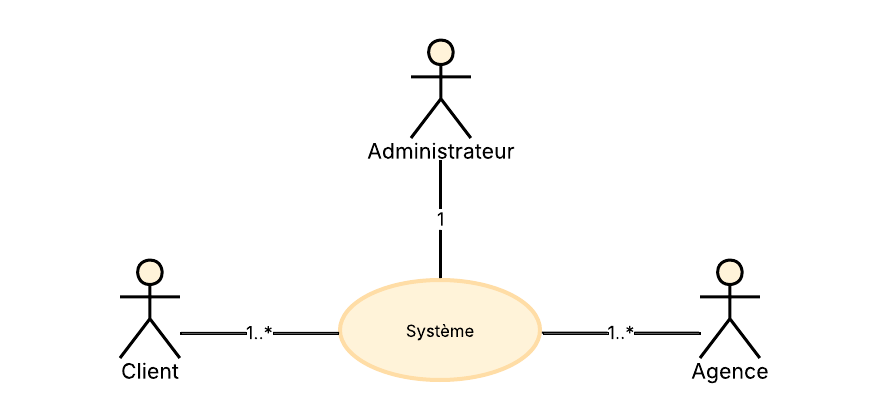
\includegraphics[width=0.7\textwidth]{Chapitres/Figures/Diag.contexte.stat.png}
    \caption{Diagramme de contexte statique}
    \label{fig:diagramme_contexte_statique}
\end{figure}

%%%%%%%%%%%%%%%%%%%%%%%%%%%%%%%%%%%%%%%%%%%%%%%%%%%%%%%%%%%%%%%%%%%%%%%%%%%
\section{Identification et analyse des besoins}
\label{section2.3}
%%%%%%%%%%%%%%%%%%%%%%%%%%%%%%%%%%%%%%%%%%%%%%%%%%%%%%%%%%%%%%%%%%%%%%%%%%%

Dans cette section, nous identifions les différentes parties prenantes du projet 
et analysons leurs besoins, qu'ils soient fonctionnels ou non fonctionnels. Cette 
étape permet de définir et d'organiser l'ensemble des exigences du système sous 
forme d'un \textbf{Product Backlog}, afin de faciliter leur gestion et leur 
priorisation pour les étapes de développement suivantes.

%%%%%%%%%%%%%%%%%%%%%%%%%%%%%%%%%%%%%%%%%%%%%%%%%%%%%%%%%%%%%%%%%%%%%%%%%%%
\subsection{Identification des besoins fonctionnels}
\label{section2.3.1}
%%%%%%%%%%%%%%%%%%%%%%%%%%%%%%%%%%%%%%%%%%%%%%%%%%%%%%%%%%%%%%%%%%%%%%%%%%%

Le besoin peut être exprimé de manière fonctionnelle, mettant en évidence les 
fonctions de services (\textit{À quoi ça sert ?}) et les fonctions techniques 
(\textit{Comment cela peut marcher ?}). Ces fonctions doivent être ordonnées, 
hiérarchisées et quantifiées sous la forme de valeurs de performance attendues.\cite{ISO}

\vspace{0.4cm}
\noindent\textbf{A. Les besoins fonctionnels de l'acteur "Internaute''}
\begin{itemize}
    \item \textbf{Consulter actualités :} L'internaute peut accéder aux informations 
    publiées sur la plateforme.
    \item \textbf{S'inscrire :} L'application permet à l'internaute de s'inscrire 
    en fournissant ses informations personnelles.
    \item \textbf{Interagir avec chatbot :} L'internaute peut poser des questions et 
    obtenir des réponses automatiques.
    \item \textbf{Contacter administrateur :} L'internaute peut envoyer un message à 
    l'administrateur pour obtenir plus d’informations .
\end{itemize}

\newpage\textbf{B. Les besoins fonctionnels de l'acteur "Utilisateur''}\\
\hspace*{0.8cm}En plus des besoins de l’acteur "Utilisateur'':
\begin{itemize}
    \item \textbf{S'authentifier :} L'utilisateur doit saisir un login et un mot de 
    passe pour accéder aux fonctionnalités de système.
    \item \textbf{Gérer profil :} L'utilisateur peut modifier ses informations 
    personnelles et ses préférences.
    \item \textbf{Consulter véhicules :} L'utilisateur peut consulter les 
    véhicules disponibles ainsi que leurs détailles.
    \item \textbf{Voir score client :} L'utilisateur peut consulter son indice de 
    fiabilité.
\end{itemize}

\textbf{C. Les besoins fonctionnels de l'acteur "Client''}\\
\hspace*{0.8cm}En plus des besoins de l’acteur "Utilisateur'':
\begin{itemize}
    \item \textbf{Effectuer réservation :} Le client peut réserver un véhicule 
    auprès d'une agence.
    \item \textbf{Consulter réservations en cours :} Le client peut suivre l'état 
    de ses réservations.
    \item \textbf{Contacter agence :} Le client peut communiquer directement avec 
    l'agence pour assistance ou négociation.
\end{itemize}

\textbf{D. Les besoins fonctionnels de l'acteur "Agence''}\\
\hspace*{0.8cm}En plus des besoins de l’acteur "Utilisateur'':
\begin{itemize}
    \item \textbf{Gérer vitrine :} L'agence peut publier et mettre à jour ses 
    véhicules disponibles.
    \item \textbf{Traiter réservations :} L'agence peut accepter ou refuser les 
    demandes de réservation ainsi que traiter les réclamations des clients..
    \item \textbf{Consulter statistiques :} L'agence peut analyser ses performances via des indicateurs.
\end{itemize}

\textbf{E. Les besoins fonctionnels de l'acteur "Administrateur''}\\
\hspace*{0.8cm}En plus des besoins de l’acteur "Utilisateur'':
\begin{itemize}
    \item \textbf{Consulter agences :} L’administrateur peut visualiser la liste des agences ainsi que leurs informations détaillées. À partir de cette interface de consultation, il peut également effectuer des actions de gestion telles que l’ajout d’une nouvelle agence, la modification des informations ou le blocage d’une agence en cas de non-conformité.
    \item \textbf{Consulter utilisateurs :} L’administrateur peut consulter les comptes la liste des utilisateurs ainsi que leurs informations. \\Depuis cette interface, il peut aussi gérer les utilisateurs en ajoutant de nouveaux comptes (en plus de l’inscription autonome), en modifiant leurs informations ou en bloquant leurs comptes si nécessaire.
    \item \textbf{Gérer messages :} L’administrateur peut consulter les messages reçus et y répondre afin d’assurer un bon suivi de la communication.
    \item \textbf{Consulter statistiques :} L’administrateur peut suivre les indicateurs de performance globaux afin de détecter les anomalies et d’améliorer le système.
\end{itemize}

%%%%%%%%%%%%%%%%%%%%%%%%%%%%%%%%%%%%%%%%%%%%%%%%%%%%%%%%%%%%%%%%%%%%%%%%%%%
\newpage
\subsection{Identification des besoins non fonctionnels}
\label{section2.3.2}
%%%%%%%%%%%%%%%%%%%%%%%%%%%%%%%%%%%%%%%%%%%%%%%%%%%%%%%%%%%%%%%%%%%%%%%%%%%

Les exigences non fonctionnelles représentent la qualité prévue de l'application et les contraintes à satisfaire lors de la réalisation des besoins fonctionnels. Notre application doit satisfaire un ensemble d'exigences non fonctionnelles :

\textbf{A. Performance}
\begin{itemize}[noitemsep, topsep=0pt]
    \item Optimiser le temps de chargement des différentes pages de l'application.
\end{itemize}
\textbf{B. Sécurité}
\begin{itemize}[noitemsep, topsep=0pt]
    \item Protéger les données personnelles des agences et des clients.
    \item Sécuriser tous les accès par authentification (login et mot de passe).
\end{itemize}
\textbf{C. Fiabilité}
\begin{itemize}[noitemsep, topsep=0pt]
    \item Garantir un fonctionnement fluide et sans erreurs critiques.
\end{itemize}
\textbf{D. Maintenabilité}
\begin{itemize}[noitemsep, topsep=0pt]
    \item Organiser le code de façon propre et structurée pour faciliter les 
    évolutions futures.
\end{itemize}
\textbf{E. Ergonomie}
\begin{itemize}[noitemsep, topsep=0pt]
    \item Offrir des interfaces intuitives, épurées et faciles à prendre en main 
    pour tous les profils d'utilisateurs.
\end{itemize}

%%%%%%%%%%%%%%%%%%%%%%%%%%%%%%%%%%%%%%%%%%%%%%%%%%%%%%%%%%%%%%%%%%%%%%%%%%%µ
\newpage
\section{Diagramme des cas d'utilisation global}
\label{section2.4}
%%%%%%%%%%%%%%%%%%%%%%%%%%%%%%%%%%%%%%%%%%%%%%%%%%%%%%%%%%%%%%%%%%%%%%%%%%%
\begin{figure}[H]
    \centering
    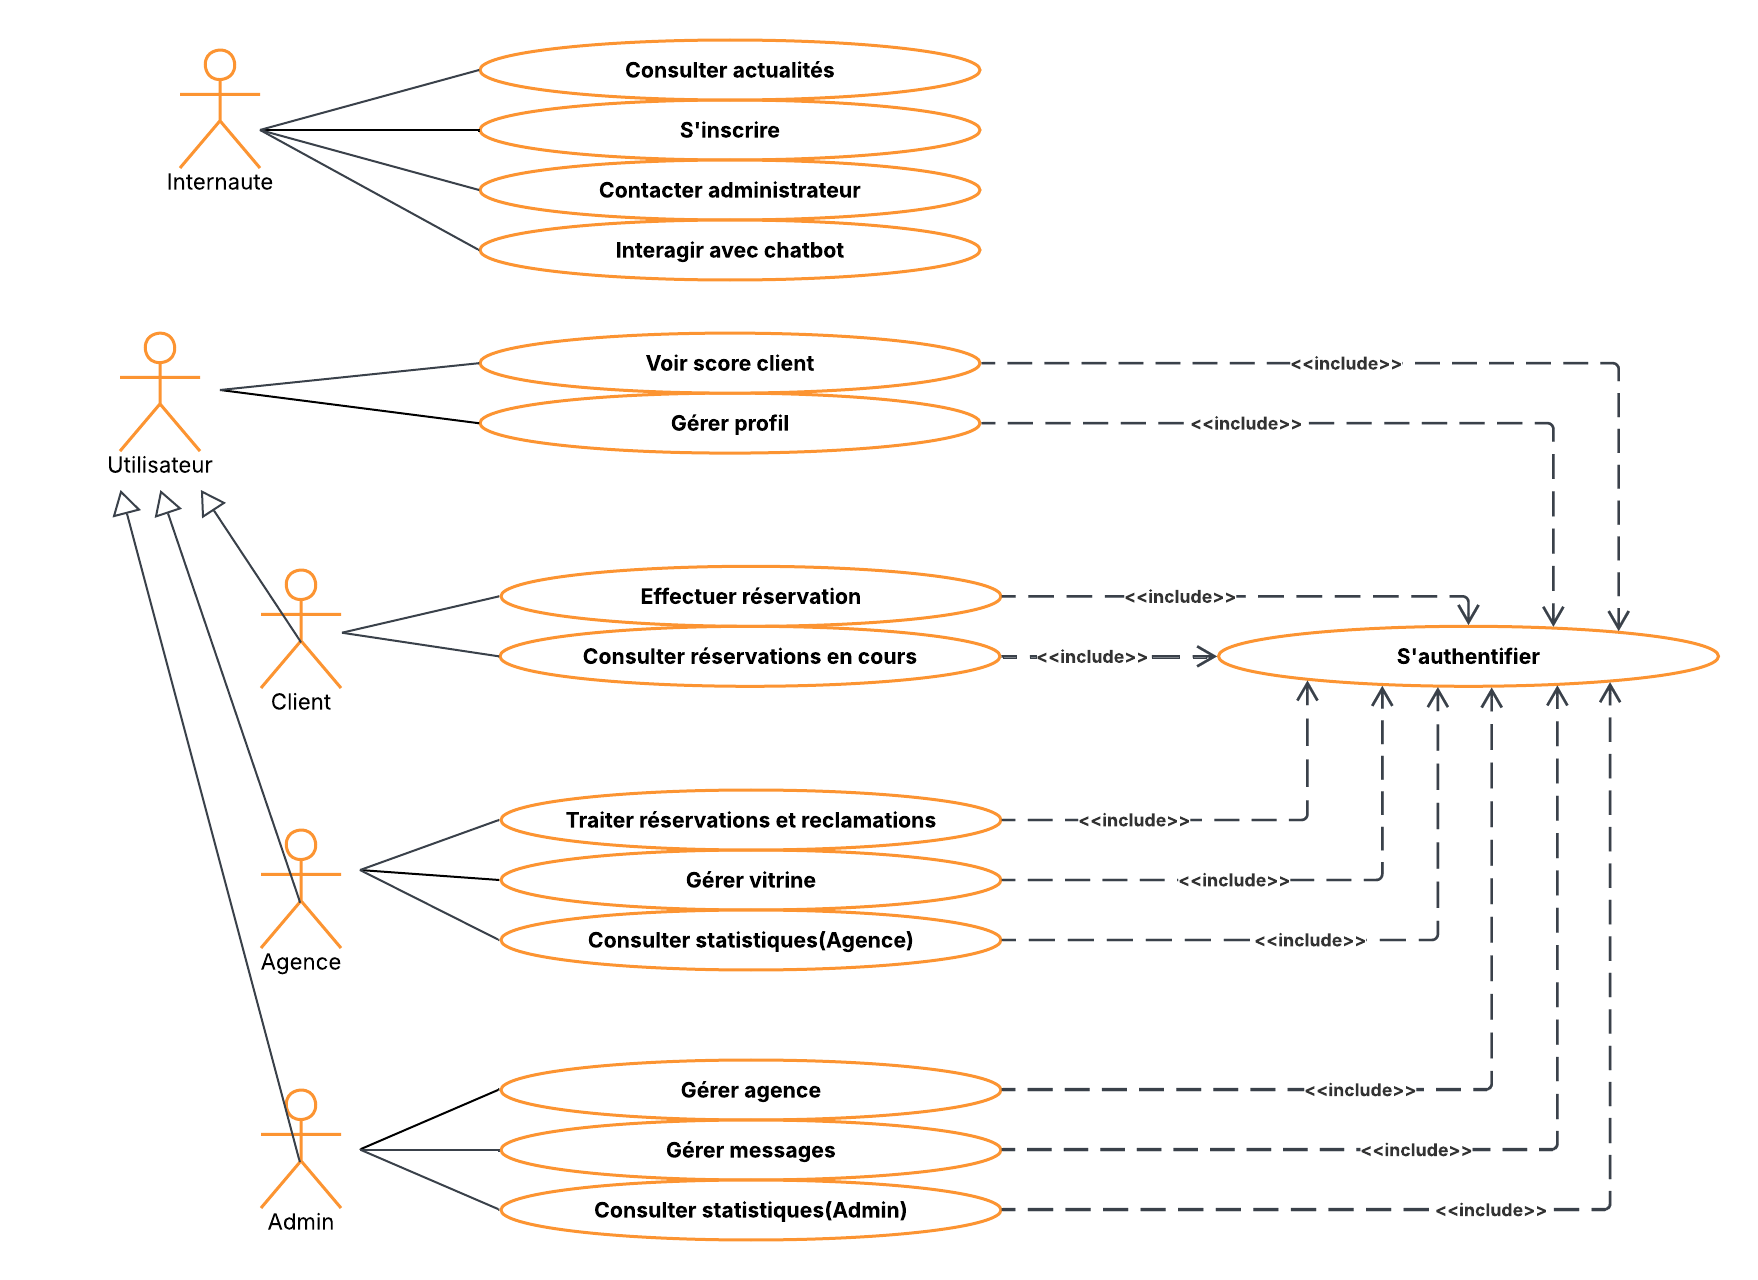
\includegraphics[width=1.2\textwidth]{Chapitres/Figures/Diag.cas.utilisation.global.png}
    \caption{Diagramme de cas d'utilisation global}
    \label{fig:cas_utilisation_global}
\end{figure}
Le diagramme de cas d'utilisation global présente une vue d'ensemble des 
interactions entre les différents acteurs (internautes, utilisateurs, clients, agences et administrateur) et notre application. Il permet de mettre en évidence les fonctionnalités principales offertes par le système ainsi que les relations hiérarchiques entre les acteurs.\cite{Lucidchart}
%%%%%%%%%%%%%%%%%%%%%%%%%%%%%%%%%%%%%%%%%%%%%%%%%%%%%%%%%%%%%%%%%%%%%%%%%%%
\newpage
\section{Identification de l'équipe Scrum}
\label{section2.5}
%%%%%%%%%%%%%%%%%%%%%%%%%%%%%%%%%%%%%%%%%%%%%%%%%%%%%%%%%%%%%%%%%%%%%%%%%%%

Dans le cadre d'une approche Scrum, il est essentiel de définir clairement les responsabilités de chaque membre de l'équipe. Les rôles Scrum structurent le travail collaboratif et garantissent une organisation efficace, assurant la transparence, la communication et l'adaptation continue tout au long du projet.

\begin{figure}[H]
    \centering
    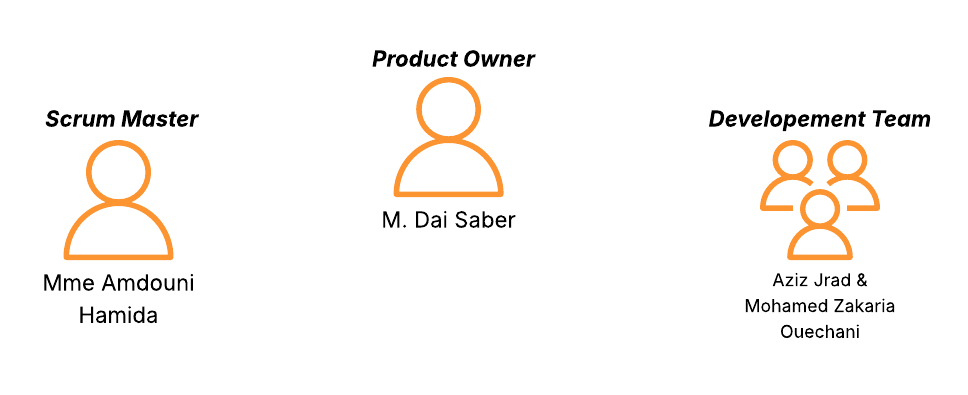
\includegraphics[width=1\textwidth]{Chapitres/Figures/Scrum-roles.png}
    \caption{Les rôles Scrum}
    \label{fig:scrum_roles}
\end{figure}

%%%%%%%%%%%%%%%%%%%%%%%%%%%%%%%%%%%%%%%%%%%%%%%%%%%%%%%%%%%%%%%%%%%%%%%%%%%
\medskip
\medskip
\medskip
\section{Le Backlog produit}
\label{section2.6}
%%%%%%%%%%%%%%%%%%%%%%%%%%%%%%%%%%%%%%%%%%%%%%%%%%%%%%%%%%%%%%%%%%%%%%%%%%%
Le \textit{Product Backlog} constitue une liste hiérarchisée de tâches qui 
définissent les caractéristiques attendues d'un produit. Il s'agit d'un élément fondamental de la méthodologie Scrum \cite{scrum}. Dans le cadre de notre projet, le backlog est structuré autour des champs suivants :
\begin{itemize}[noitemsep, topsep=3pt]
    \item \textbf{ID :} identifiant unique attribué à chaque \textit{User Story}, permettant de la distinguer et de la référencer facilement dans le backlog.
    \item \textbf{Thème :} résumé synthétique décrivant la fonctionnalité concernée, servant de regroupement logique pour plusieurs \textit{User Stories} liées.
    \item \textbf{User Story :} description du contenu fonctionnel attendu, exprimée du point de vue de l'utilisateur, sous forme de scénario simple.
    \item \textbf{Priorité :} niveau d'importance défini par le \textit{Product Owner}, indiquant l’ordre de traitement et la valeur métier associée à la fonctionnalité.
\end{itemize}

\newpage
\renewcommand{\arraystretch}{1}

\begin{longtable}{|c|c|c|p{4cm}|c|}
\caption{Backlog produit}
\label{tab:backlogproduit} \\

\hline
\textbf{Id} & \textbf{Thème} & \textbf{En tant que} & \textbf{User Story (Je veux...)} & \textbf{Priorité} \\
\hline
\endfirsthead

\hline
\textbf{Id} & \textbf{Thème} & \textbf{En tant que} & \textbf{User Story (Je veux...)} & \textbf{Priorité} \\
\hline
\endhead

\hline
\endfoot

\hline
\endlastfoot

US01 & Actualités & Internaute & consulter les actualités afin d'accéder aux informations publiées sur la plateforme & Moyenne \\ \hline
US02 & Gestion des comptes & Internaute & s'inscrire afin d'accéder aux services & Haute \\ \hline
US03 & Assistance & Internaute & interagir avec le chatbot afin d'obtenir des réponses automatiques & Moyenne \\ \hline
US04 & Support & Internaute & contacter l'administrateur afin d'obtenir plus d’informations & Haute \\ \hline
US05 & Chatbot & Internaute & interagir avec le chatbot afin d'obtenir des réponses automatiques & Moyenne \\ \hline


US06 & Authentification & Utilisateur & m'authentifier afin d'accéder aux fonctionnalités du système & Haute \\ \hline
US07 & Profil & Utilisateur & gérer mon profil afin de modifier mes informations personnelles et préférences & Moyenne \\ \hline
US08 & Véhicules & Utilisateur & consulter les véhicules disponibles ainsi que leurs détails & Haute \\ \hline
US09 & Score client & Utilisateur & voir mon score afin de connaître mon indice de fiabilité & Moyenne \\ \hline

US10 & Réservations & Client & effectuer une réservation afin de louer un véhicule auprès d'une agence & Haute \\ \hline
US11 & Réservations & Client & consulter mes réservations en cours afin de suivre leur état & Haute \\ \hline
US12 & Vitrine & Agence & gérer la vitrine afin de publier et mettre à jour les véhicules disponibles & Haute \\ \hline
US13 & Réservations & Agence & traiter les réservations afin d'accepter ou refuser les demandes et gérer les réclamations & Haute \\ \hline
US14 & Statistiques & Agence & consulter les statistiques afin d'analyser les performances & Moyenne \\ \hline

US15 & Consultation des agences & Admin & consulter les agences afin de visualiser, ajouter, modifier ou bloquer les agences & Haute \\ \hline
US16 & Consultation des utilisateurs & Admin & consulter les utilisateurs afin de visualiser, ajouter, modifier ou bloquer les comptes & Haute \\ \hline
US17 & Messages & Admin & gérer les messages afin de consulter et répondre aux utilisateurs & Moyenne \\ \hline
US18 & Statistiques globales & Admin & consulter les statistiques globales afin d'analyser les performances du système & Haute \\ \hline

\end{longtable}
%%%%%%%%%%%%%%%%%%%%%%%%%%%%%%%%%%%%%%%%%%%%%%%%%%%%%%%%%%%%%%%%%%%%%%%%%%%
\newpage
\section{La planification des sprints}
\label{section2.7}
%%%%%%%%%%%%%%%%%%%%%%%%%%%%%%%%%%%%%%%%%%%%%%%%%%%%%%%%%%%%%%%%%%%%%%%%%%%

La planification de sprint permet d'identifier les tâches qui seront accomplies pendant le sprint et la manière dont elles seront réalisées. 

\begin{figure}[H]
    \centering
    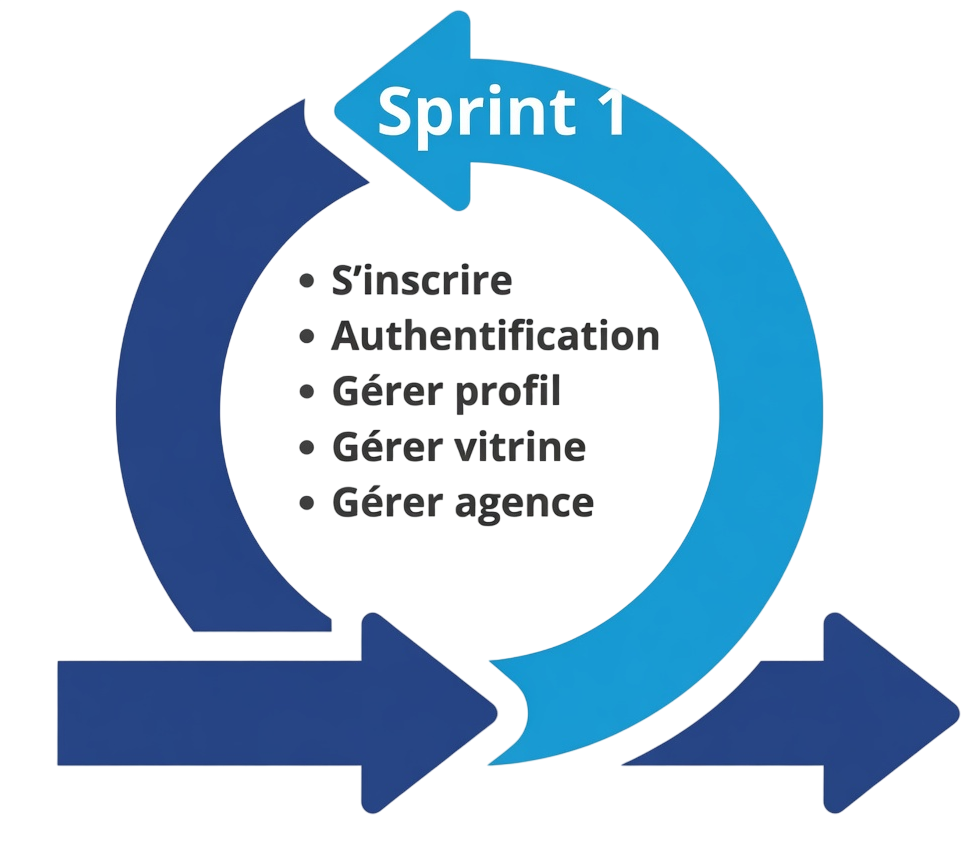
\includegraphics[width=0.7\textwidth]{Chapitres/Figures/sprint_1.png}
    \caption{Sprint 1}
    \label{fig:sprint_1}
\end{figure}
\begin{figure}[H]
    \centering
    \includegraphics[width=1\textwidth]{Chapitres/Figures/sprint_2.png}
    \caption{Sprint 2}
    \label{fig:sprint_2}
\end{figure}
%%%%%%%%%%%%%%%%%%%%%%%%%%%%%%%%%%%%%%%%%%%%%%%%%%%%%%%%%%%%%%%%%%%%%%%%%%%
\section{Diagramme de Gantt}
\label{section2.8}
%%%%%%%%%%%%%%%%%%%%%%%%%%%%%%%%%%%%%%%%%%%%%%%%%%%%%%%%%%%%%%%%%%%%%%%%%%%
Le diagramme de Gantt illustre la répartition temporelle des quatre phases du projet sur une durée totale de douze semaines.

\begin{figure}[H]
    \centering
    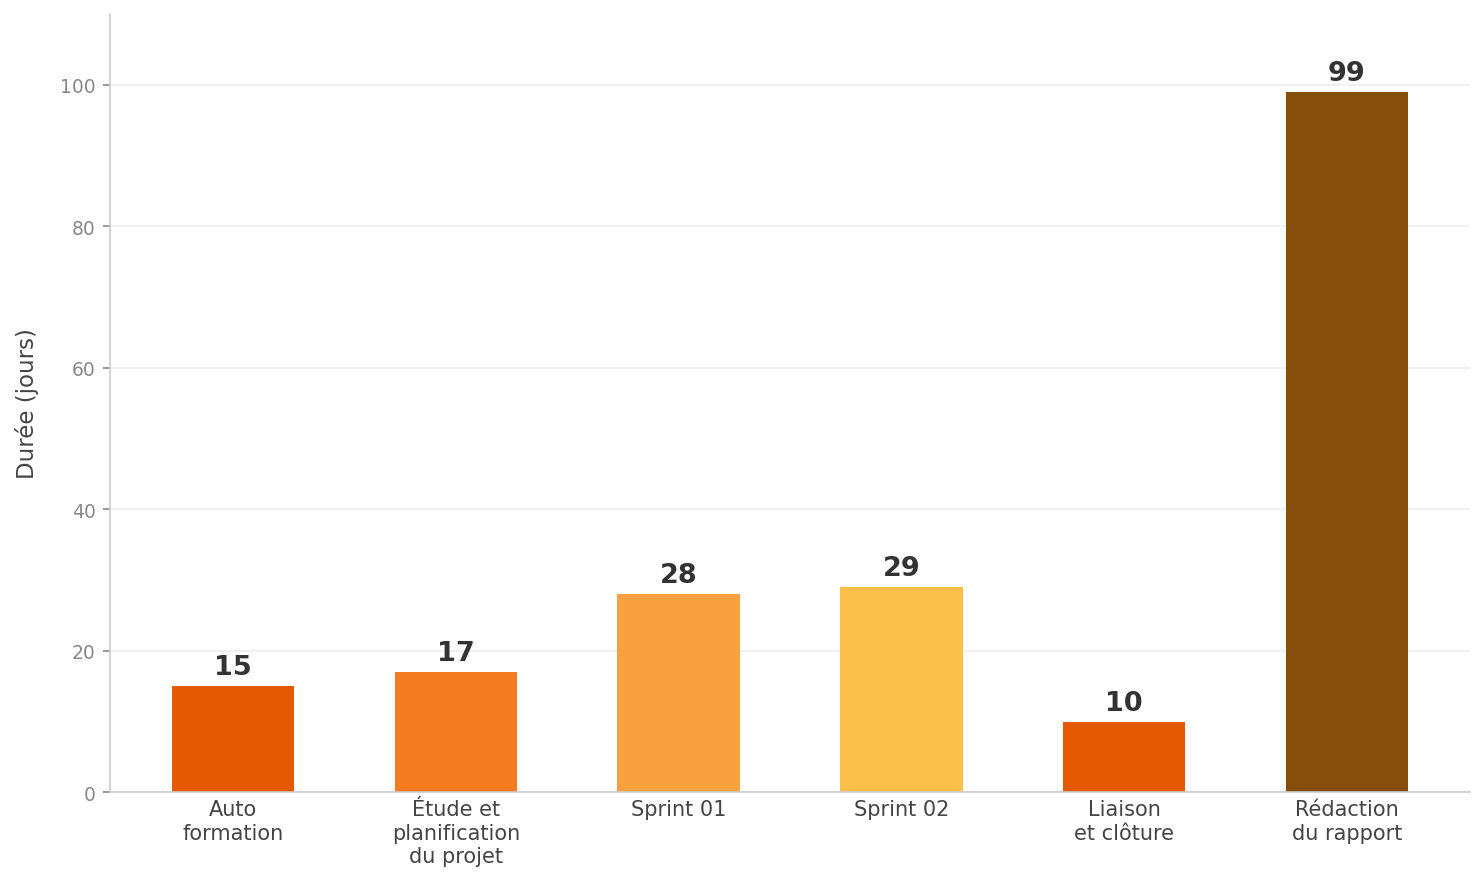
\includegraphics[width=1\textwidth]{Chapitres/Figures/gantt.png}
    \caption{Diagramme de Gantt}
    \label{fig:gantt}
\end{figure}

%%%%%%%%%%%%%%%%%%%%%%%%%%%%%%%%%%%%%%%%%%%%%%%%%%%%%%%%%%%%%%%%%%%%%%%%%%%
\section{Conclusion}
%%%%%%%%%%%%%%%%%%%%%%%%%%%%%%%%%%%%%%%%%%%%%%%%%%%%%%%%%%%%%%%%%%%%%%%%%%%

Au cours de ce chapitre, nous avons identifié les parties prenantes et défini le backlog du produit en précisant les demandes fonctionnelles et techniques de notre projet.

\medskip

Ensuite, nous avons achevé la première étape de la méthodologie Scrum en constituant l'équipe, en élaborant le diagramme global des cas d'utilisation et en établissant la liste des tâches produit ainsi que la planification des sprints.

\medskip

Le chapitre suivant sera consacré à la réalisation du \textbf{Sprint 1}, couvrant la gestion des agences, des clients et de la vitrine.
\raggedbottom
\chapter{Réalisation du premier sprint}
\label{Chapitre_3}

{\Large\textbf{Sprint : Gérer les intervenants}}

%%%%%%%%%%%%%%%%%%%%%%%%%%%%%%%%%%%%%%%%%%%%%%%%%%%%%%%%%%%%%%%%%%%%%%%%%%%
\section{Introduction}
\label{Chapitre3_Introduction}
%%%%%%%%%%%%%%%%%%%%%%%%%%%%%%%%%%%%%%%%%%%%%%%%%%%%%%%%%%%%%%%%%%%%%%%%%%%
En se basant sur la planification établie dans le chapitre précédent, ce chapitre est consacré à la réalisation du Sprint 1. Nous aborderons successivement la description fonctionnelle, la conception, l'implémentation et la phase de tests.


%%%%%%%%%%%%%%%%%%%%%%%%%%%%%%%%%%%%%%%%%%%%%%%%%%%%%%%%%%%%%%%%%%%%%%%%%%%
\section{Backlog produit du premier sprint}
\label{sec:backlog_sprint1}
%%%%%%%%%%%%%%%%%%%%%%%%%%%%%%%%%%%%%%%%%%%%%%%%%%%%%%%%%%%%%%%%%%%%%%%%%%%

Le Sprint Backlog est constitué d'une série de tâches définies par l'équipe 
et devant être complétées avant la clôture du sprint.\cite{atlassian}

\begin{table}[H]
\centering
\caption{Backlog produit du premier sprint}
\label{tab:backlog-sprint1}
\renewcommand{\arraystretch}{1.4}
\resizebox{\textwidth}{!}{%
\begin{tabular}{|l|c|l|p{4cm}|p{5cm}|c|}
\hline
\textbf{Acteur} & \textbf{ID tâche} & \textbf{Thème} & \textbf{User Story} & \textbf{Tâche} & \textbf{Estimation (Jours)} \\
\hline

\multirow{5}{*}{Internaute}
& US01 & S'inscrire 
& S'inscrire afin d'accéder aux services
& Rédiger les spécifications et diagrammes du cas «S'inscrire». & \multirow{3}{*}{4} \\
\cline{5-5}
& & & & Implémenter l'inscription. & \\
\cline{5-5}
& & & & Tester. & \\
\cline{2-6}

& US06 & Consulter actualités 
& Consulter les actualités
& Implémenter l'affichage des actualités. & \multirow{2}{*}{3} \\
\cline{5-5}
& & & & Tester. & \\
\cline{2-6}

& US07 & Contacter administrateur 
& Contacter l'administrateur
& Implémenter le formulaire de contact. & \multirow{2}{*}{3} \\
\cline{5-5}
& & & & Tester. & \\
\hline

\multirow{4}{*}{Utilisateur}
& US02 & Authentification 
& S'authentifier afin d'accéder au système
& Rédiger les diagrammes du cas «S'authentifier». & \multirow{2}{*}{4} \\
\cline{5-5}
& & & & Implémenter l'authentification et tester. & \\
\cline{2-6}

& US03 & Gérer profil 
& Gérer mon profil
& Implémenter la consultation et modification du profil. & \multirow{2}{*}{4} \\
\cline{5-5}
& & & & Tester. & \\
\hline

\multirow{2}{*}{Agence}
& US04 & Gérer vitrine 
& Gérer la vitrine
& Implémenter la gestion de la vitrine. & \multirow{2}{*}{4} \\
\cline{5-5}
& & & & Tester. & \\
\hline

\multirow{4}{*}{Administrateur}
& US05 & Gérer agences 
& Gérer les agences afin de visualiser, ajouter, modifier ou bloquer
& Implémenter la gestion des agences. & \multirow{4}{*}{4} \\
\cline{5-5}
& & & & Tester. & \\
\cline{2-6}

& US08 & Gérer messages 
& Gérer les messages
& Implémenter la gestion des messages. & \multirow{2}{*}{2} \\
\cline{5-5}
& & & & Tester. & \\
\hline
\multicolumn{5}{|r|}{\textbf{Estimation Totale (Jours)}} & \textbf{28} \\ \hline
\end{tabular}%
}
\end{table}
%%%%%%%%%%%%%%%%%%%%%%%%%%%%%%%%%%%%%%%%%%%%%%%%%%%%%%%%%%%%%%%%%%%%%%%%%%%
%section
\newpage
\section{Les prototypes des interfaces}
\label{sec:prototypes_interfaces}
Prototyper aide à identifier forces, faiblesses et à limiter les risques.%%%%%%%%%%%%%%%%%%%%%%%%%%%%%%%%%%%%%%%%%%%%%%%%%%%%%%%%%%%%%%%%%%%%%%%%%%%
\begin{figure}[H]
    \centering
    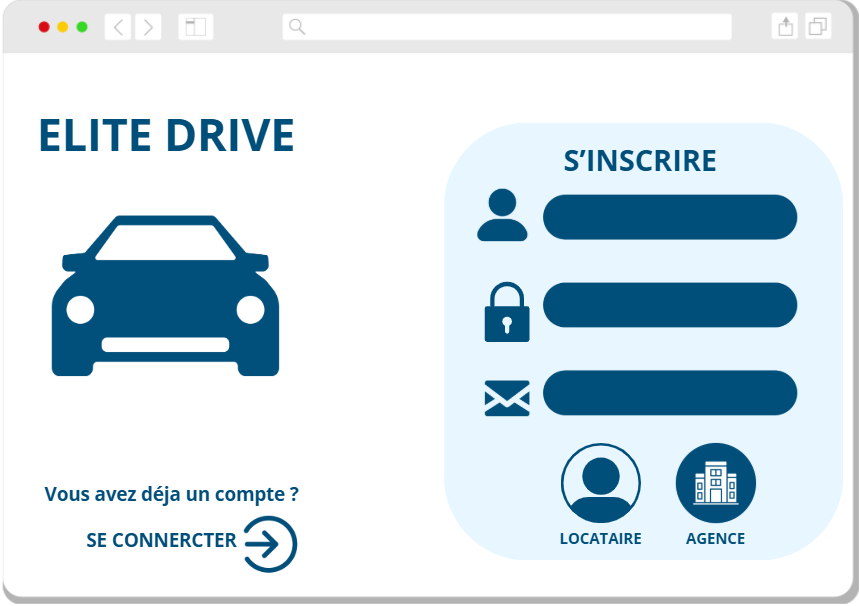
\includegraphics[width=0.8\textwidth]{Chapitres/Figures/proto_inscription.png}
    \caption{Prototypage de l'interface d'inscription}
    \label{fig:proto_inscription}
\end{figure}
\begin{figure}[H]
    \centering
    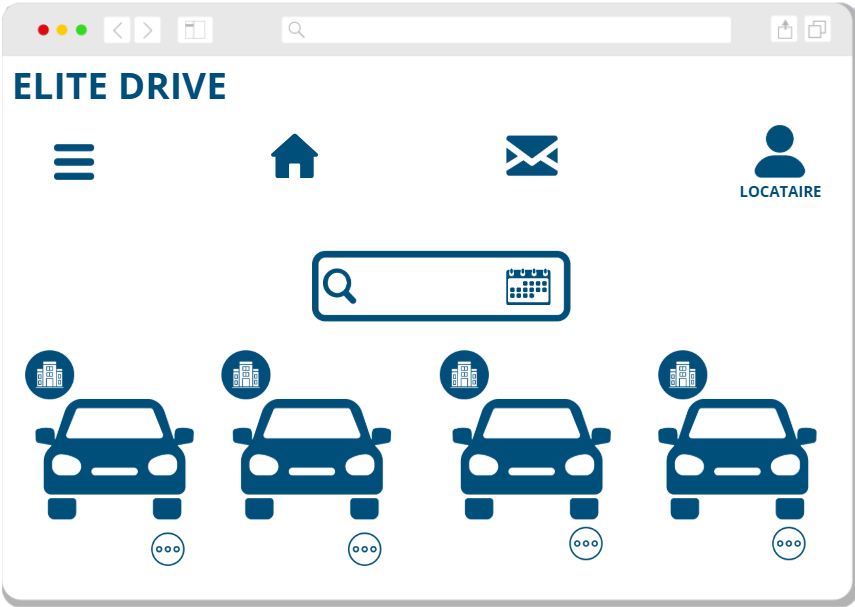
\includegraphics[width=0.8\textwidth]{Chapitres/Figures/proto_client.png}
    \caption{Prototypage de l'interface «Utilisateur»}
    \label{fig:proto_client}
\end{figure}

\clearpage
%%%%%%%%%%%%%%%%%%%%%%%%%%%%%%%%%%%%%%%%%%%%%%%%%%%%%%%%%%%%%%%%%%%%%%%%%%%
%section
\section{La spécification fonctionnelle des besoins}
\label{sec:besoins}
On décide d'étudier la spécification fonctionnelle en analysant les diagrammes de cas d'utilisation détaillés du premier sprint, ainsi que les descriptions textuelles et les diagrammes système associés à chaque fonctionnalité.

%%%%%%%%%%%%%%%%%%%%%%%%%%%%%%%%%%%%%%%%%%%%%%%%%%%%%%%%%%%%%%%%%%%%%%%%%%%
%section
\section{Diagramme de cas d'utilisation du premier sprint}
\label{sec:diag_cas_sprint1}
La figure suivante présente le diagramme des cas d'utilisation du premier sprint.
%%%%%%%%%%%%%%%%%%%%%%%%%%%%%%%%%%%%%%%%%%%%%%%%%%%%%%%%%%%%%%%
%figure
\begin{figure}[H]
    \centering
    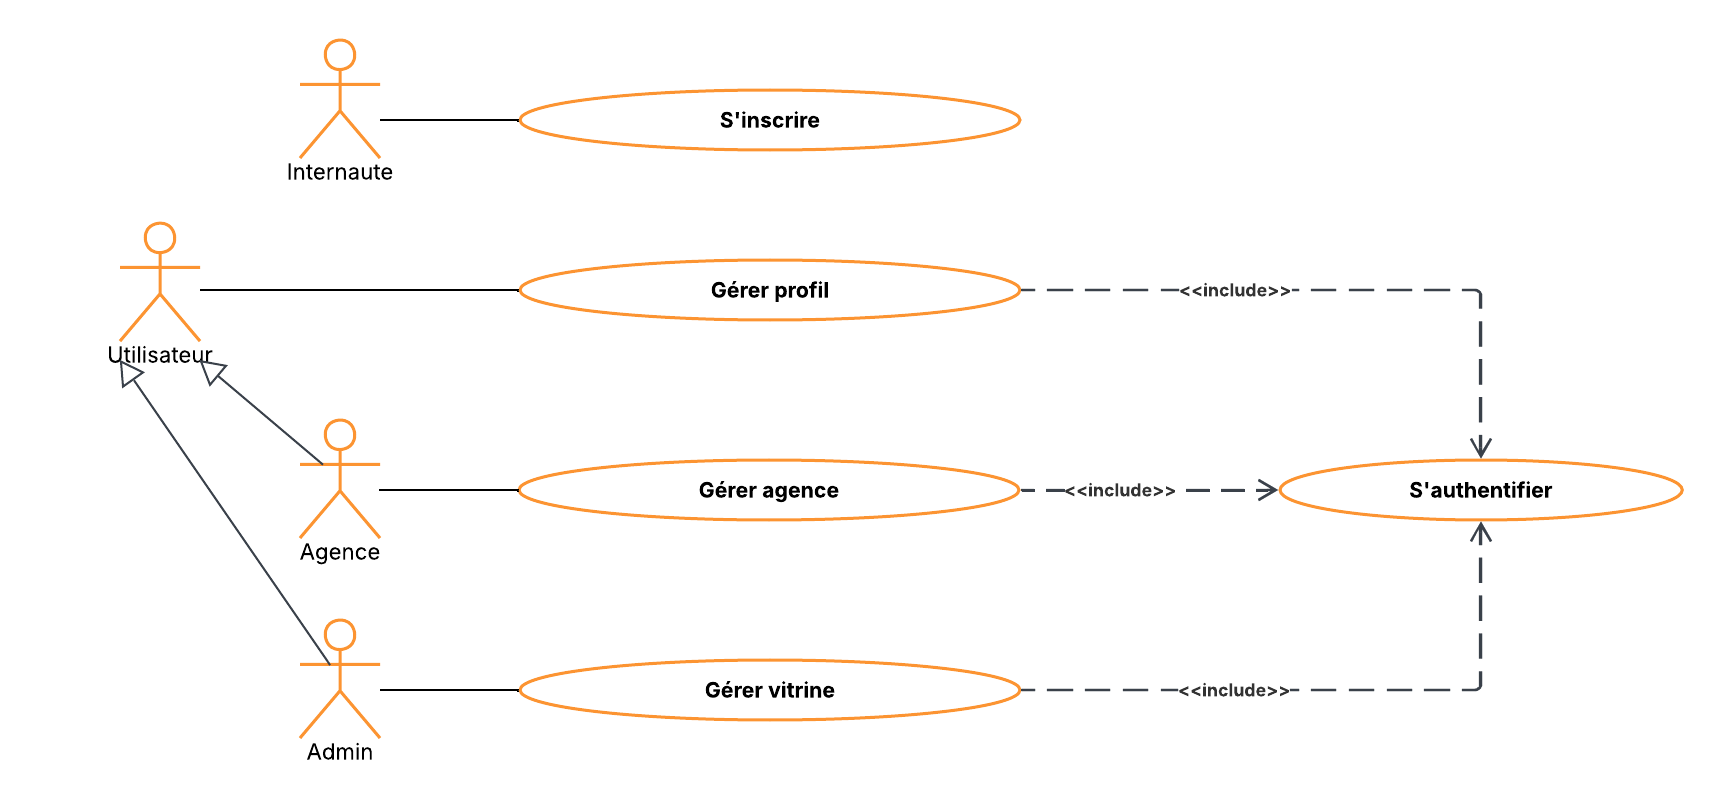
\includegraphics[width=1\textwidth]{Chapitres/Figures/diag_cas_sprint1.png}
    \caption{Diagramme de cas d'utilisation du premier sprint}
    \label{fig:Diag_use_case_S1}
\end{figure}
\newpage
\section{Analyse des cas d'utilisation du premier sprint}
\label{sec:sprint1}
À chaque cas d'utilisation, nous allons associer une description textuelle pour détailler le scénario ainsi que les éventuelles situations exceptionnelles.

%%%%%%%%%%%%%%%%%%%%%%%%%%%%%%%%%%%%%%%%%%%%%%%%%%%%%%%%%%%%%%%
\section{Analyse des cas d'utilisation de l'acteur «Internaute»}
\label{sec:use_case_acteur_internaute}
%%%%%%%%%%%%%%%%%%%%%%%%%%%%%%%%%%%%%%%%%%%%%%%%%%%%%%%%%%%%%%%
\subsection{Analyse de cas d'utilisation «Consulter actualités»}
\label{sec:cons_act}
Afin de mieux illustrer le déroulement du scénario, nous proposons ci‑après une description textuelle accompagnée du diagramme de séquence du cas d'utilisation \textbf{«Consulter actualités»}.
\begin{table}[H]
\centering
\caption{Description textuelle du cas d'utilisation «Consulter actualités»}
\label{tab:consulter_actualites}
\renewcommand{\arraystretch}{1.3}
\resizebox{\textwidth}{!}{%
\begin{tabular}{|l|p{11cm}|}
\hline
\textbf{Élément} & \textbf{Description} \\
\hline
Acteur & Internaute \\
\hline
Description & Permet à l’internaute de consulter les dernières actualités publiées sur la plateforme.\\
\hline
Précondition & L’internaute accède à la plateforme.\newline Des actualités sont disponibles. \\
\hline
Postcondition & L’internaute visualise les actualités.\newline Il peut accéder au détail d’une actualité. \\
\hline
Scénario nominal & 1. L’internaute accède à la section actualités.\newline
2. Le système affiche la liste des actualités.\newline
3. L’internaute sélectionne une actualité.\newline
4. Le système affiche le contenu détaillé. \\
\hline
Scénarios alternatifs & 
Pas d'exceptions\\
\hline
\end{tabular}
}
\end{table}
\begin{figure}[H]
    \centering
    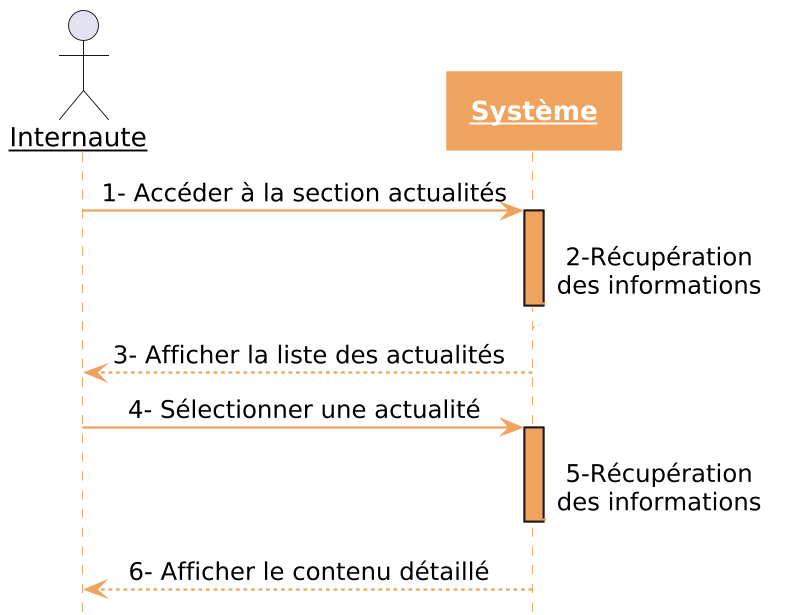
\includegraphics[width=0.7\textwidth]{Chapitres/Figures/Diag_seq_consulter_act.png}
    \caption{Diagramme de séquence système de cas d'utilisation «Consulter actualités»}
    \label{fig:consulter_actualites}
\end{figure}
%%%%%%%%%%%%%%%%%%%%%%%%%%%%%%%%%%%%%%%%%%%%%%%%%%%%%%%%%%%%%%%%
\subsection{Analyse de cas d'utilisation «S'inscrire»}
\label{sec:s_inscrire}
Afin de mieux illustrer le déroulement du scénario, nous proposons ci‑après une description textuelle accompagnée du diagramme de séquence du cas d'utilisation 
\textbf{«S'inscrire»}.

\begin{table}[htbp]
\centering
\caption{Description textuelle du cas d'utilisation «S'inscrire»}
\label{tab:s_inscrire}
\renewcommand{\arraystretch}{1.3}
\resizebox{\textwidth}{!}{%
\begin{tabular}{|l|p{11cm}|}
\hline
\textbf{Élément} & \textbf{Description} \\
\hline
Acteur & Internaute \\
\hline
Pré-condition & L'internaute consulte le site de l'application. \\
\hline
Post-condition & L'internaute est enregistré. \\
\hline
Scénario nominal &
1. L'internaute lance l'application. \newline
2. L'internaute sélectionne l'option «S'inscrire». \newline
3. Le système affiche le formulaire d'inscription. \newline
4. L'internaute remplit le formulaire. \newline
5. Le système vérifie les données saisies. \newline
6. L'internaute valide l'inscription. \newline
7. Le système vérifie l'unicité de l'e-mail. \newline
8. Le système redirige l'internaute vers le formulaire de connexion. \\
\hline
\multirow{9}{*}{\textbf{Scénario alternatif}} & 
5.1 Données manquantes ou incorrectes. \\
& \quad 5.1.1 Le système affiche un message d'erreur. \\
& \quad 5.1.2 Retour à l'étape 4 du scénario nominal. \\
& 5.2 Données invalides. \\
& \quad 5.2.1 Le système affiche un message d'erreur. \\
& \quad 5.2.2 Retour à l'étape 4 du scénario nominal. \\
& 7.1 Internaute déjà inscrit. \\
& \quad 7.1.1 Le système affiche un message d'erreur. \\
& \quad 7.1.2 Retour à l'étape 4 du scénario nominal. \\
\hline
\end{tabular}%
}
\end{table}

\begin{figure}[H]
    \centering
    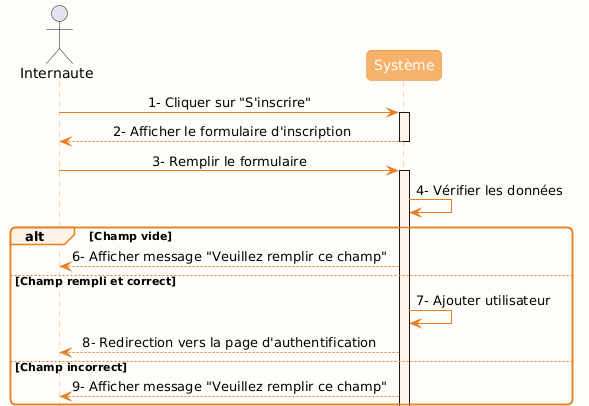
\includegraphics[width=0.7\textwidth]{Chapitres/Figures/diag_seq_s_inscrire.png}
    \caption{Diagramme de séquence système de cas d'utilisation «S'inscrire»}
    \label{fig:s_inscrire}
\end{figure}
%%%%%%%%%%%%%%%%


%%%%%%%%%%%%%%%%%%%%%%%%%%%%%%%%%%%%%%%%%%%%%%%%%%%%%%%%%%%%%%%
\subsection{Analyse de cas d'utilisation «Contacter administrateur»}
\label{sec:contacter_admin}
Afin de mieux illustrer le déroulement du scénario, nous proposons ci‑après une description textuelle accompagnée du diagramme de séquence du cas d'utilisation 
\textbf{«Contacter administrateur»}.

\begin{table}[htbp]
\centering
\caption{Description textuelle du cas d'utilisation «Contacter administrateur»}
\label{tab:contacter_admin}
\renewcommand{\arraystretch}{1.3}
\resizebox{\textwidth}{!}{%
\begin{tabular}{|l|p{11cm}|}
\hline
\textbf{Élément} & \textbf{Description} \\
\hline
Acteur & Internaute \\
\hline
Pré-condition & L'internaute accède au site de l'application. \newline
Le système est accessible. \\
\hline
Post-condition & Le message est envoyé à l’administrateur. \newline
Le système affiche un message de confirmation. \\
\hline
Scénario nominal &
1. L’internaute accède à la page «Contact». \newline
2. Le système affiche le formulaire de contact. \newline
3. L’internaute saisit les informations demandées et le message. \newline
4. L’internaute clique sur «Envoyer». \newline
5. Le système vérifie les données saisies. \newline
6. Le système envoie le message à l’administrateur. \newline
7. Le système affiche un message de confirmation. \\
\hline
\multirow{4}{*}{\textbf{Scénarios alternatifs}} 
& 5.1 Champs invalides ou incomplets. \\
& \quad 5.1.1 Le système affiche un message d’erreur. \\
& 6.1 Échec lors de l’envoi du message. \\
& \quad 6.1.1 Le système affiche un message d’échec. \\
\hline
\end{tabular}%
}
\end{table}

\begin{figure}[H]
    \centering
    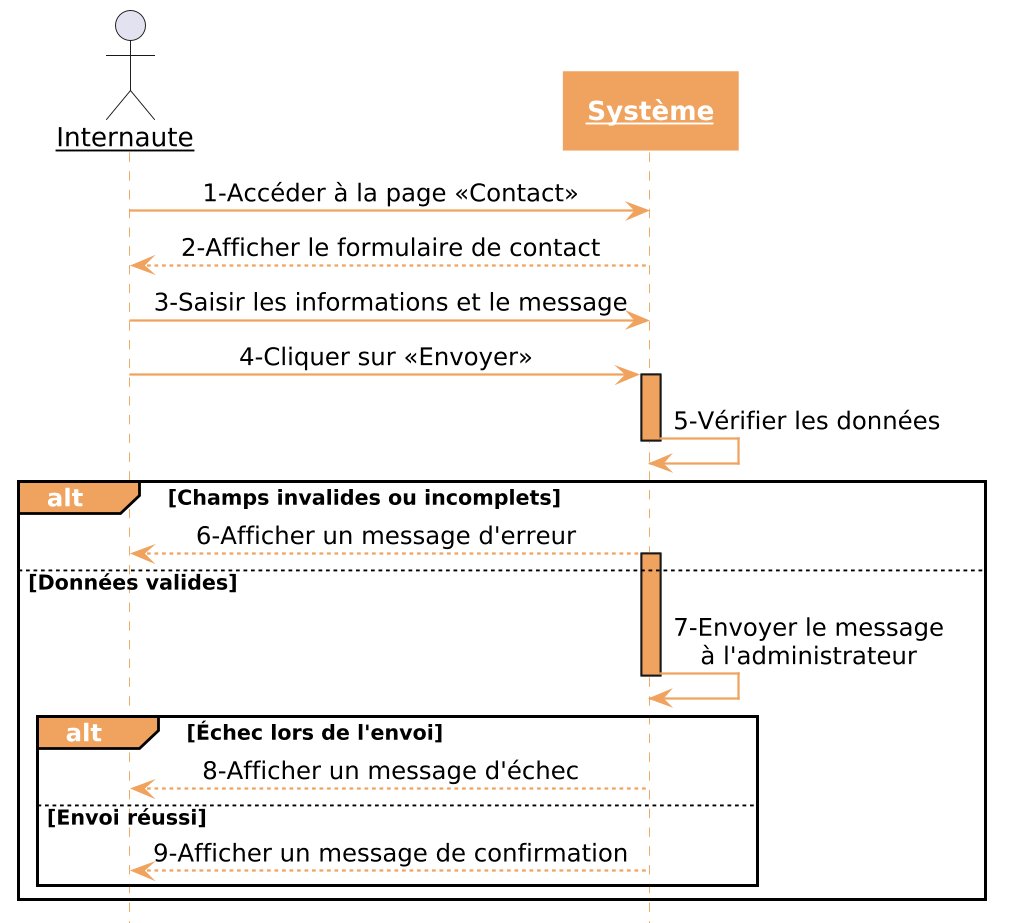
\includegraphics[width=0.7\textwidth]{Chapitres/Figures/diag_seq_contacter_admin.png}
    \caption{Diagramme de séquence système de cas d'utilisation «Contacter administrateur»}
    \label{fig:contacter_admin}
\end{figure}
%%%%%%%%%%%%%%%%%%%%%%%%%%%%%%%%%%%%%%%%%%%%%%%%%%%%%%%%%%%%%%%
\section{Analyse des cas d'utilisation de l'acteur «Utilisateur»}
\label{sec:acteur_utilisateur}
%%%%%%%%%%%%%%%%%%%%%%%%%%%%%%%%%%%%%%%%%%%%%%%%%%%%%%%%%%%%%%%
\subsection{Analyse de cas d'utilisation «S'authentifier»}
\label{sec:authentifier}
Afin de mieux illustrer le déroulement du scénario, nous proposons ci‑après une description textuelle accompagnée du diagramme de séquence du cas d'utilisation \textbf{«S'authentifier»}.
\begin{table}[htbp]
\centering
\caption{Description textuelle du cas d'utilisation «S'authentifier»}
\label{tab:authentifier}
\renewcommand{\arraystretch}{1.4}
\resizebox{\textwidth}{!}{%
\begin{tabular}{|l|p{11cm}|}
\hline
\textbf{Cas d'utilisation} & S'authentifier \\
\hline
\textbf{Acteur} & Utilisateur \\
\hline
\textbf{Pré-condition} & L'utilisateur a déjà un compte. \\
\hline
\textbf{Post-condition} & Utilisateur authentifié. \\
\hline
\multirow{8}{*}{\textbf{Scénario nominal}} & 1. L'utilisateur lance l'application.\\
& 2. L'utilisateur sélectionne l'option «Se connecter».\\
& 3. Le système fait apparaître le formulaire de connexion.\\
& 4. L'utilisateur entre son adresse de courrier électronique et son mot de passe.\\
& 5. Le système vérifie les données saisies.\\
& 6. L'utilisateur sélectionne l'option «Se connecter».\\
& 7. Le système examine la présence des informations saisies.\\
& 8. Le système redirige l'utilisateur vers son espace personnel.\\
\hline
\multirow{6}{*}{\textbf{Scénario alternatif}} & 5.1 L'utilisateur insère des données manquantes et/ou incorrectes.\\
& \quad 5.1.1 Le système fait apparaître un message d'erreur.\\
& \quad 5.1.2 Retour à l'étape 3 du scénario nominal.\\
& 5.2 Le compte est inexistant.\\
& \quad 5.2.1 Le système fait apparaître un message d'erreur.\\
& \quad 5.2.2 Retour à l'étape 3 du scénario nominal.\\
\hline
\end{tabular}%
}
\end{table}

\begin{figure}[H]
    \centering
    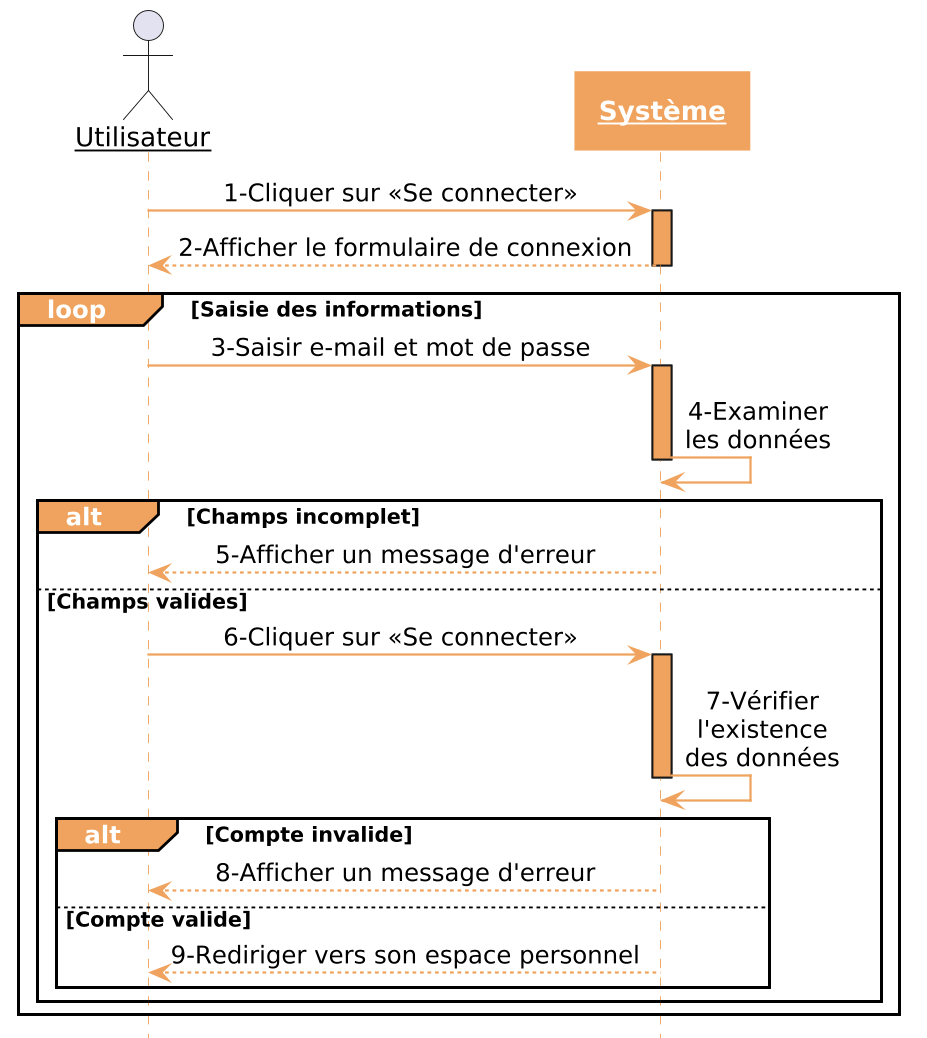
\includegraphics[width=1\textwidth]{Chapitres/Figures/diag_seq_s_authentifier.png}
    \caption{Diagramme de séquence système de cas d'utilisation «S'authentifier»}
    \label{fig:authentifier}
\end{figure}

%%%%%%%%%%%%%%%%%%%%%%%%%%%%%%%%%%%%%%%%%%%%%%%%%%%%
\newpage
\subsection{Analyse de cas d'utilisation «Gérer profil»}
\label{sec:gerer_profil}
La section suivante présente le raffinement du cas d’utilisation «Gérer profil» de l’acteur \textit{Utilisateur}.
\begin{figure}[H]
    \centering
    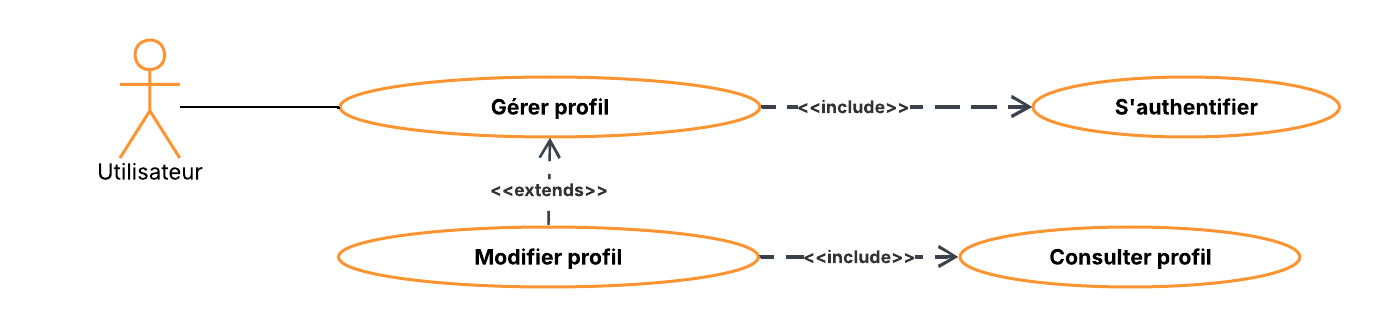
\includegraphics[width=1\textwidth]{Chapitres/Figures/Diag_cas_Gerer_profil.png}
    \caption{Raffinement du cas d'utilisation «Gérer profil»}
    \label{fig:Diag_gerer_profil}
\end{figure}


%%%%%%%%%%%%%%%%%%%%%%%%%%%%%
\subsubsection{Analyse de cas d'utilisation «Consulter profil»}
\label{sec:consulter_profil}
La section suivante propose une description textuelle et un diagramme de séquence, auxquels s'ajoute l'analyse du cas d'utilisation \textbf{«Consulter profil»} de l'acteur \textbf{Utilisateur}.

\begin{table}[htbp]
\centering
\caption{Description textuelle du cas d'utilisation «Consulter profil»}
\label{tab:consulter_profil}
\renewcommand{\arraystretch}{1.3}
\resizebox{\textwidth}{!}{%
\begin{tabular}{|l|p{11cm}|}
\hline
\textbf{Élément} & \textbf{Description} \\
\hline
Nom & Consulter profil \\
\hline
Acteur & Utilisateur \\
\hline
Description brève & Permet à un utilisateur de consulter son profil. \\
\hline
Précondition & 
L'utilisateur est authentifié. \newline
Le système est accessible. \\
\hline
Postcondition & 
Ensemble des données affichés. \\
\hline
Enchaînement principal & 
1. L'utilisateur clique sur «Profil». \newline
2. Le système affiche les informations du profil. \\
\hline
Scénarios alternatifs & 
Pas d'exceptions\\
\hline
\end{tabular}%
}
\end{table}

\begin{figure}[H]
    \centering
    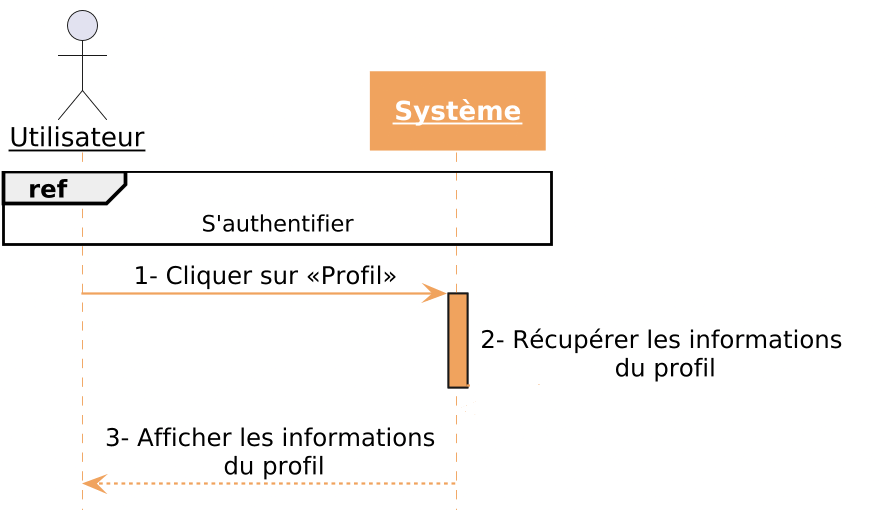
\includegraphics[width=0.7\textwidth]{Chapitres/Figures/diag_seq_consulter_profil.png}
    \caption{Diagramme de séquence système de cas d'utilisation «Consulter profil»}
    \label{fig:consulter_profil}
\end{figure}

\subsubsection{Analyse de cas d'utilisation «Modifier profil»}
\label{sec:modifier_profil}
La section suivante propose une description textuelle et un diagramme de séquence, auxquels s'ajoute l'analyse du cas d'utilisation \textbf{«Modifier profil»} de l'acteur \textbf{Utilisateur}.

\begin{table}[htbp]
\centering
\caption{Description textuelle du cas d'utilisation «Modifier profil»}
\label{tab:modifier_profil}
\renewcommand{\arraystretch}{1.3}
\resizebox{\textwidth}{!}{%
\begin{tabular}{|l|p{11cm}|}
\hline
\textbf{Élément} & \textbf{Description} \\
\hline
Nom & Modifier profil \\
\hline
Acteur & Utilisateur \\
\hline
Description brève & Permet à un utilisateur de modifier ses informations personnelles (nom, email, mot de passe, numéro de téléphone). \\
\hline
Précondition & 
L'utilisateur est authentifié. \newline
Le système est accessible. \\
\hline
Postcondition & 
Les informations du profil sont mises à jour. \newline
Les nouvelles données sont enregistrées. \\
\hline
Enchaînement principal & 
1. L'utilisateur accède à la page «profil». \newline
2. Le système affiche les informations actuelles du profil. \newline
3. L'utilisateur modifie ses informations personnelles. \newline
4. Le système vérifie les données et effectue la modification. \newline
5. Le système affiche un message de confirmation. \\
\hline
\multirow{4}{*}{\textbf{Scénarios alternatifs}} 
& 4.1 Informations invalides. \\
& \quad 4.1.1 Le système affiche un message d'erreur. \\
& 5.1 Échec lors de l'enregistrement. \\
& \quad 5.1.1 Le système affiche un message d'échec. \\
\hline
\end{tabular}%
}
\end{table}
\begin{figure}[H]
    \centering
    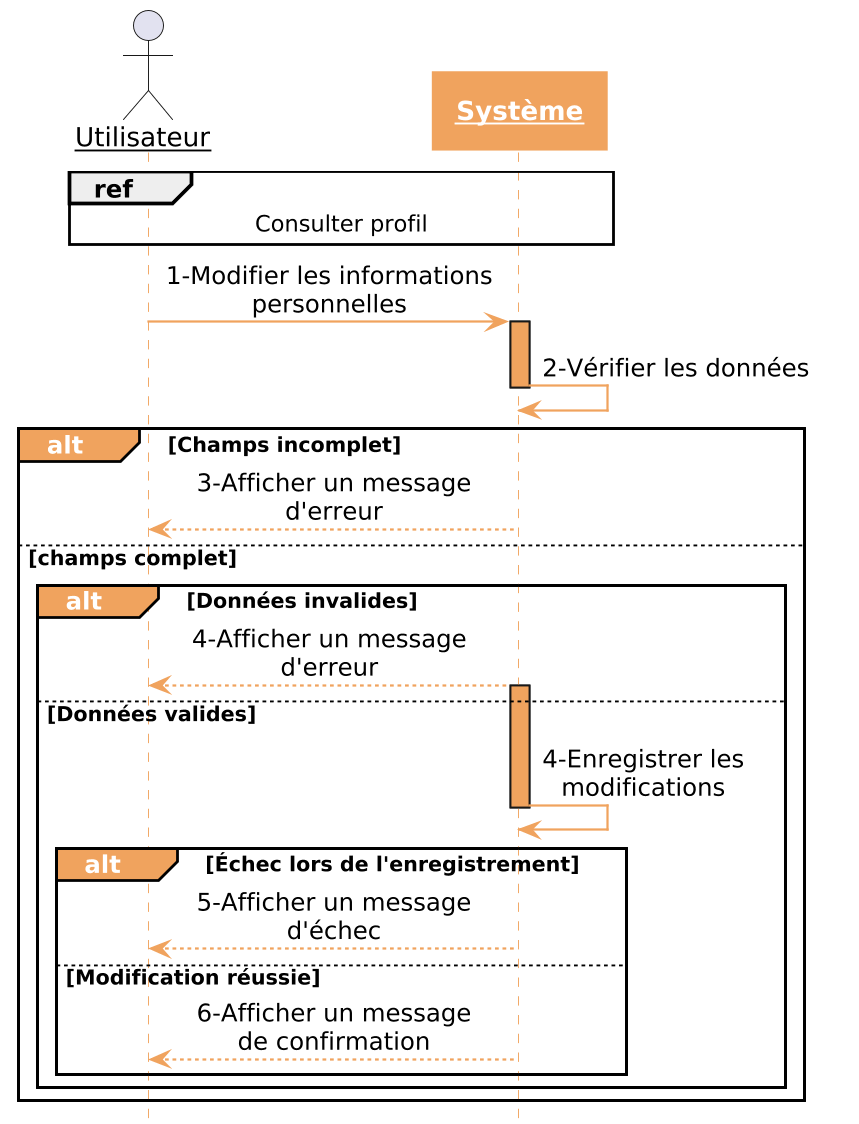
\includegraphics[width=0.7\textwidth]{Chapitres/Figures/diag_seq_modifier_profil.png}
    \caption{Diagramme de séquence système de cas d'utilisation «Modifier profil»}
    \label{fig:modifier_profil}
\end{figure}

%%%%%%%%%%%%%%%%%%%%%%%%%%%%%
%%%%%%1111%%%%%%%%%


%%%%%%%%%%44444444444%%%%%%%%%%%%%%%%%%%%%%%%
\FloatBarrier
\section{Analyse des cas d'utilisation de l'acteur «Administrateur»}
\label{sec:acteur_admin}
%%%%%%%%%%%%%%%%%%%%%%%%%%%%%%%%%%%%%%%%%%%%%%%%%%%%%%%%%%%%%%%

\subsection{Analyse de cas d'utilisation «Gérer agences»}
\label{sec:gerer_agences}
Afin de mieux illustrer le déroulement du scénario, nous proposons ci‑après un raffinement du cas d'utilisation \textbf{«Gérer agences»} de l'acteur \textit{Administrateur}.

\begin{figure}[H]
    \centering
    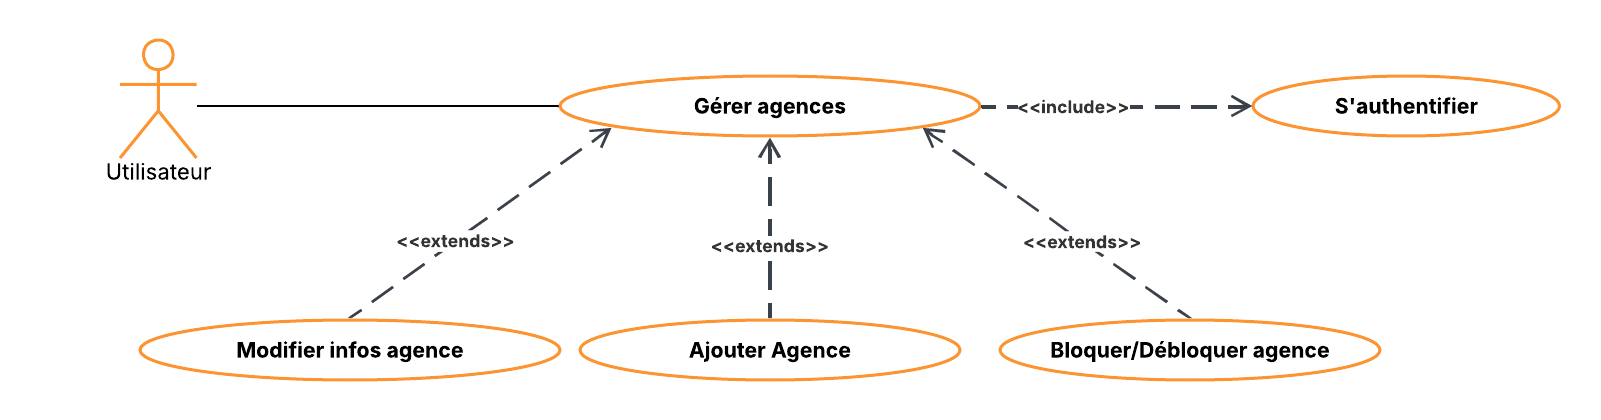
\includegraphics[width=1\textwidth]{Chapitres/Figures/raf_gerer_agences.png}
    \caption{Raffinement du cas d'utilisation «Gérer agences»}
    \label{fig:raf_gerer_agences}
\end{figure}
%%%%%%%%%%%%%%
\subsubsection{Analyse de cas d'utilisation «Consulter agences»}
\label{sec:consulter_agences}
La section suivante propose une description textuelle et un diagramme de séquence, auxquels s'ajoute l'analyse du cas d'utilisation \textbf{«Consulter agences»} de l'acteur \textbf{Administrateur}.

\begin{table}[htbp]
\centering
\caption{Description textuelle du cas d'utilisation «Consulter agences»}
\label{tab:consulter_agences}
\renewcommand{\arraystretch}{1.3}
\resizebox{\textwidth}{!}{%
\begin{tabular}{|l|p{11cm}|}
\hline
\textbf{Élément} & \textbf{Description} \\
\hline
Nom & Consulter agences \\
\hline
Acteur & Administrateur \\
\hline
Description brève & Permet à un administrateur de consulter les informations des agences. \\
\hline
Précondition & 
L'administrateur est authentifié. \newline
Le système est accessible. \\
\hline
Postcondition & 
Ensemble des données affichés. \\
\hline
Enchaînement principal & 
1. L'administrateur clique sur «Agences». \newline
2. Le système affiche les informations des agences. \\
\hline
Scénarios alternatifs & 
Pas d'exceptions\\
\hline
\end{tabular}%
}
\end{table}

\begin{figure}[H]
    \centering
    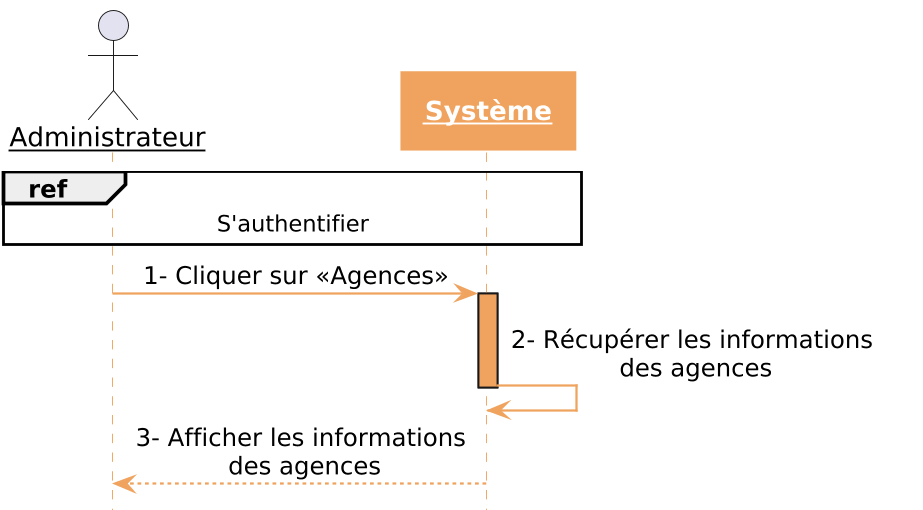
\includegraphics[width=0.7\textwidth]{Chapitres/Figures/diag_seq_consulter_agences.png}
    \caption{Diagramme de séquence système de cas d'utilisation «Consulter agences»}
    \label{fig:consulter_agences}
\end{figure}

%%%%%%%%%%%%%%
\subsubsection{Analyse de cas d'utilisation «Modifier infos agence»}
\label{sec:modifier_infos_agence}
La section suivante propose une description textuelle et un diagramme de séquence, auxquels s'ajoute l'analyse du cas d'utilisation \textbf{«Modifier infos agence»} de l'acteur \textbf{Administrateur}.

\begin{table}[htbp]
\centering
\caption{Description textuelle du cas d'utilisation «Modifier infos agence»}
\label{tab:modifier_infos_agence}
\renewcommand{\arraystretch}{1.3}
\resizebox{\textwidth}{!}{%
\begin{tabular}{|l|p{11cm}|}
\hline
\textbf{Élément} & \textbf{Description} \\
\hline
Nom & Modifier infos agence \\
\hline
Acteur & Administrateur \\
\hline
Description brève & Permet à un administrateur de modifier les informations d'une agence. \\
\hline
Précondition & 
L'administrateur est authentifié. \newline
Le système est accessible. \\
\hline
Postcondition & 
Les informations de l'agence sont mises à jour. \newline
Les nouvelles données sont enregistrées. \\
\hline
Enchaînement principal & 
1. L'administrateur accède à la page «gestion des agences». \newline
2. Le système affiche les informations actuelles de l'agence. \newline
3. L'administrateur modifie les informations de l'agence. \newline
4. Le système vérifie les données et effectue la modification. \newline
5. Le système affiche un message de confirmation. \\
\hline
\multirow{4}{*}{\textbf{Scénarios alternatifs}} 
& 4.1 Informations invalides. \\
& \quad 4.1.1 Le système affiche un message d'erreur. \\
& 5.1 Échec lors de l'enregistrement. \\
& \quad 5.1.1 Le système affiche un message d'échec. \\
\hline
\end{tabular}%
}
\end{table}
\begin{figure}[H]
    \centering
    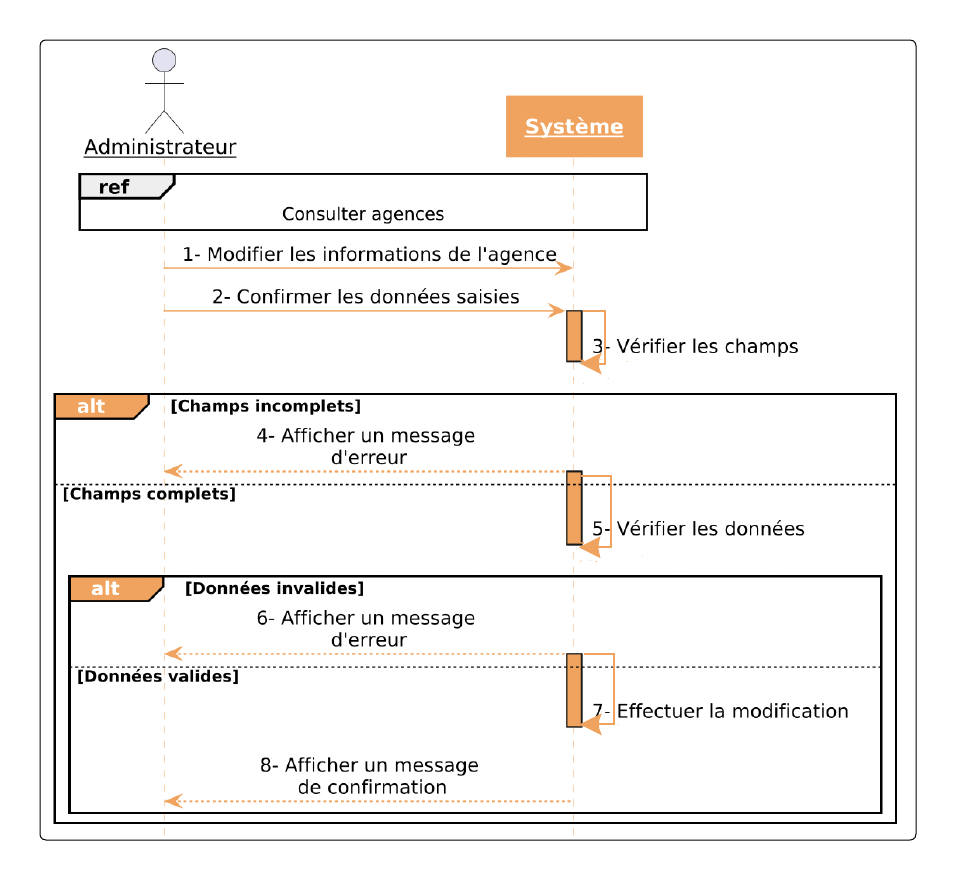
\includegraphics[width=0.7\textwidth]{Chapitres/Figures/diag_seq_modifier_infos_agences.png}
    \caption{Diagramme de séquence système de cas d'utilisation «Modifier infos agence»}
    \label{fig:modifier_infos_agences}
\end{figure}

%%%%%%%%%%%%%%%%    
\FloatBarrier
\subsection{Analyse de cas d'utilisation «Ajouter agence»}
\label{sec:ajouter_agence}
Dans la suite, nous présentons une description textuelle accompagnée d'un diagramme 
de séquence du cas d'utilisation \textbf{«Ajouter agence»} de l'acteur 
\textbf{Administrateur}.
\begin{table}[htbp]
\centering
\caption{Description textuelle du cas d'utilisation «Ajouter agence»}
\label{tab:ajouter_agence}
\renewcommand{\arraystretch}{1.3}
\resizebox{\textwidth}{!}{%
\begin{tabular}{|l|p{11cm}|}
\hline
\textbf{Élément} & \textbf{Description} \\
\hline
Nom & ajouter agence \\
\hline
Acteur & Administrateur \\
\hline
Description brève & Permet à l'administrateur d'ajouter une agence. \\
\hline
Précondition & 
 L'administrateur est authentifié. \newline
 Le système est accessible. \\
\hline
Postcondition & 
 Une agence est ajoutée. \\
\hline
Enchaînement principal & 
1. L'administrateur accède à la page de gestion. \newline
2. Le système affiche la liste des agence. \newline
3. L'administrateur clique sur «ajouter une agence». \newline
4. Le système affiche le formulaire d'ajout. \newline
5. L'administrateur saisit les informations nécessaires. \newline
6. Le système vérifie les données. \newline
7. Le système enregistre l'agence. \newline
8. Le système affiche un message de confirmation. \\
\hline
\multirow{6}{*}{\textbf{Scénario alternatif}} & 6.1 Informations invalides.\\
& \quad 6.1.1 Le système affiche un message d'erreur. \\
& 7.1 Erreur lors de l'enregistrement. \\
& \quad 7.1.1 Le système affiche un message d'échec. \\
\hline
\end{tabular}%
}
\end{table}

\begin{figure}[H]
    \centering
    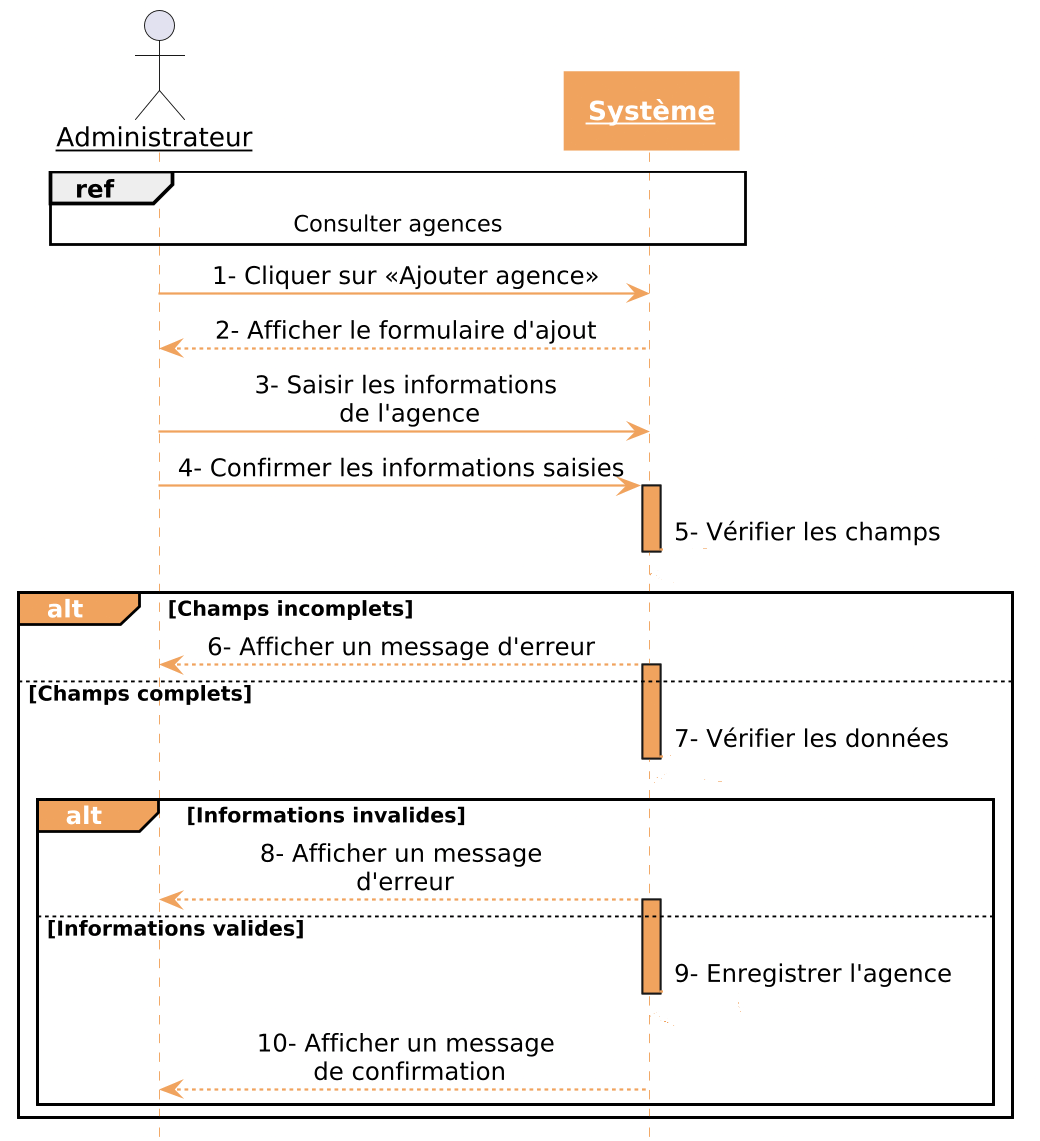
\includegraphics[width=1\textwidth]{Chapitres/Figures/Diag_seq_ajouter_agence.png}
    \caption{Diagramme de séquence système de cas d'utilisation «Ajouter agence»}
    \label{fig:ajouter_agence}
\end{figure}

\FloatBarrier
\subsection{Analyse de cas d'utilisation «Bloquer/Débloquer agence»}
\label{sec:bloquer/debloquer_agence}
Dans la suite, nous présentons une description textuelle accompagnée d'un diagramme 
de séquence du cas d'utilisation \textbf{«Bloquer/Débloquer agence»} de l'acteur 
\textbf{Administrateur}.

\begin{table}[H]
\centering
\caption{Description textuelle du cas d'utilisation «Bloquer/Débloquer agence»}
\label{tab:use-case-bloquer-agence}
\renewcommand{\arraystretch}{1.3}
\begin{tabular}{|l|p{10cm}|}
\hline
\textbf{Élément} & \textbf{Description} \\
\hline
Nom & Bloquer/Débloquer agence \\
\hline
Acteur & Administrateur \\
\hline
Description brève & Permet à l'administrateur de bloquer ou de débloquer une agence afin de désactiver ou d'activer son accès. \\
\hline
Précondition & 
 L'administrateur est authentifié. \newline
 L'agence existe dans le système. \\
\hline
Postcondition & 
 L'agence est bloquée/Débloquée et peut/ ne peut plus accéder au système. \\
\hline
Enchaînement principal & 
1. L'administrateur consulte la liste des agences. \newline
2. L'administrateur sélectionne une agence. \newline
3. L'administrateur clique sur «Bloquer/Débloquer». \newline
4. Le système demande confirmation. \newline
5. L'administrateur confirme. \newline
6. Le système bloque/débloque l'agence. \newline
7. Le système affiche un message de confirmation. \\
\hline
\multirow{4}{*}{\textbf{Scénario alternatif}} 
& 5.1 Annulation de l'action. \\
& \quad 5.1.1 Aucune modification n'est effectuée. \\
& 6.1 Erreur lors du blocage/déblocage. \\
& \quad 6.1.1 Le système affiche un message d'échec. \\
\hline
\end{tabular}
\end{table}

\begin{figure}[H]
    \centering
    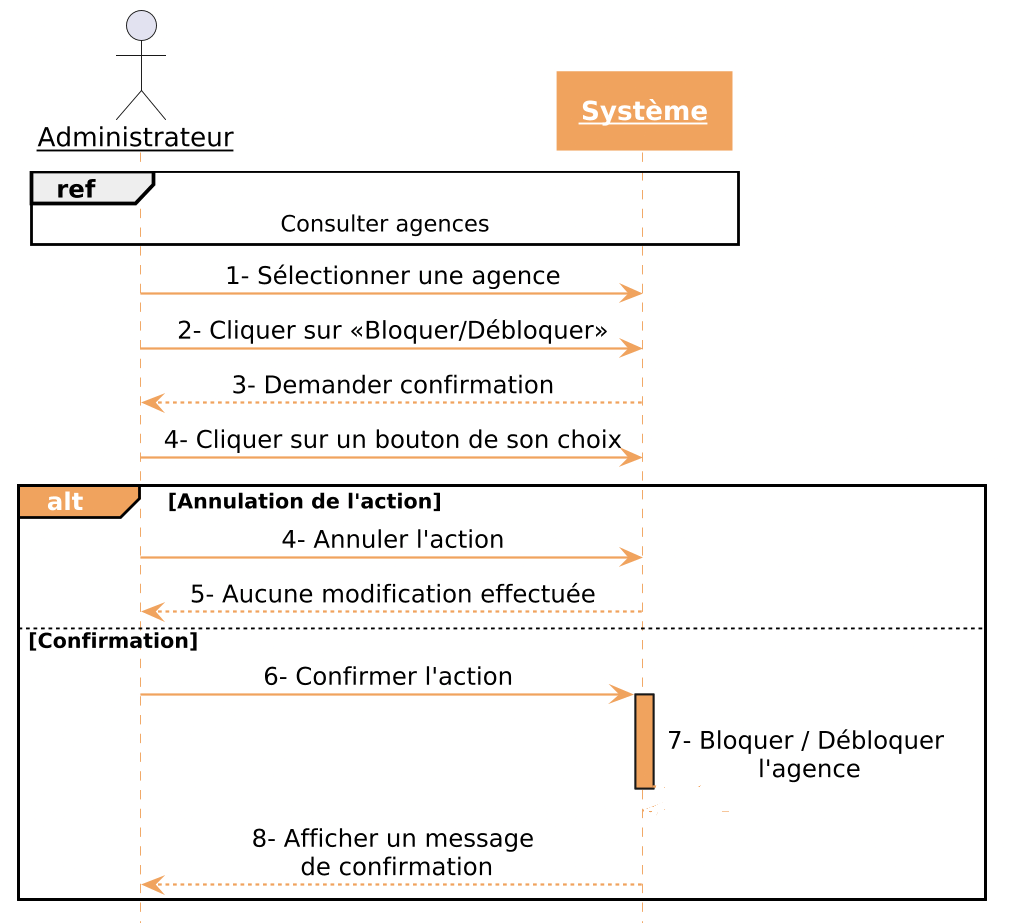
\includegraphics[width=1\textwidth]{Chapitres/Figures/Diag_seq_bloquer_agence.png}
    \caption{Diagramme de séquence système de cas d'utilisation «Bloquer agences»}
    \label{fig:bloquer_agences}
\end{figure}

\subsection{Analyse de cas d'utilisation "Gérer messages''}
\label{sec:gerer_messages}

Afin de mieux illustrer le déroulement du scénario, nous proposons ci-après une analyse
du cas d'utilisation "\textbf{Gérer messages}'' de l'acteur Administrateur.

\begin{table}[H]
\centering
\caption{Description textuelle du cas d'utilisation "Gérer messages''}
\label{tab:gerer_messages}
\renewcommand{\arraystretch}{1.35}
\begin{tabular}{|p{3.5cm}|p{10cm}|}
\hline
\textbf{Élément} & \textbf{Description} \\
\hline
Nom & Gérer messages \\
\hline
Acteur & Administrateur \\
\hline
Description brève & Permet à l'administrateur de consulter les messages reçus des utilisateurs et d'y apporter une réponse. \\
\hline
Précondition & L'administrateur est authentifié. \newline
               Le système est accessible. \\
\hline
Postcondition & Le message est traité et une réponse est envoyée à l'utilisateur concerné. \\
\hline
Enchaînement principal &
1. L'administrateur accède à la section "~Messages~''. \newline
2. Le système affiche la liste des messages reçus avec leur statut. \newline
3. L'administrateur sélectionne un message. \newline
4. Le système affiche le contenu du message et les informations de l'expéditeur. \newline
5. L'administrateur rédige une réponse. \newline
6. Le système enregistre et envoie la réponse. \newline
7. Le système marque le message comme traité et affiche un message de confirmation. \\
\hline
\textbf{Scénario alternatif} &
6.1 Erreur lors de l'envoi de la réponse. \newline
\quad 6.1.1 Le système affiche un message d'échec. \\
\hline
\end{tabular}
\end{table}

\begin{figure}[H]
    \centering
    
\includegraphics[width=1\textwidth]{Chapitres/figures/seq_gerer_messages.png}
    \caption{Diagramme de séquence système de cas d'utilisation "Gérer messages''}
    \label{fig:seq_gerer_messages}
\end{figure}

%%%%%%%%%%%%%%%%%%%%%%%%%%%%%%%%%%%%%%%%%%%%%%%%%%%%%%%%%%%%%%%
\newpage
\FloatBarrier
\section{Analyse des cas d'utilisation de l'acteur «Agence»}
\label{sec:acteur_agence}
%%%%%%%%%%%%%%%%%%%%%%%%%%%%%%%%%%%%%%%%%%%%%%%%%%%%%%%%%%%%%%%

\subsection{Analyse de cas d'utilisation «Gérer vitrine»}
\label{sec:gerer_vitrine}
Pour mieux analyser le déroulement du scénario, nous proposons ci‑après un 
raffinement accompagné d'une description textuelle et un diagramme de séquence du cas d'utilisation \textbf{«Gérer vitrine»} de l'acteur \textit{Agence}.

\begin{figure}[H]
    \centering
    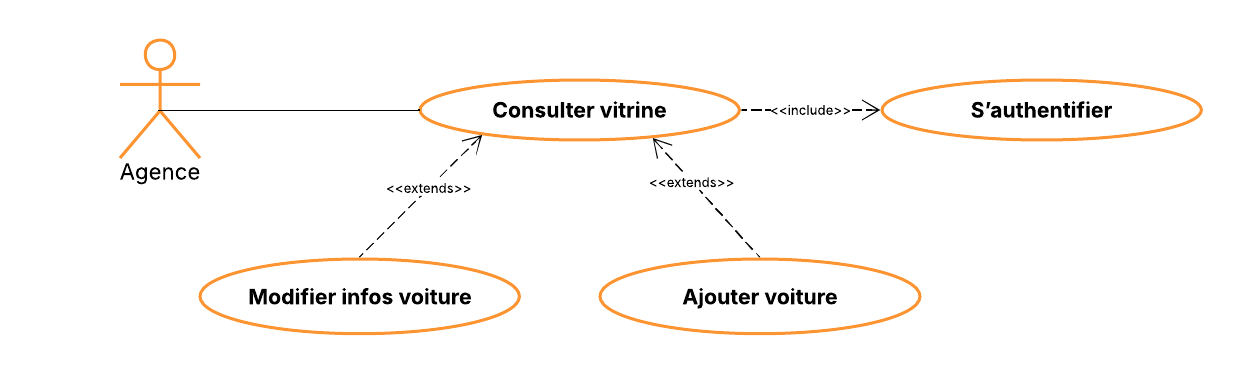
\includegraphics[width=1\textwidth]{Chapitres/Figures/raf_gerer_vitrine.png}
    \caption{Raffinement du cas d'utilisation «Gérer vitrine»}
    \label{fig:raf_gerer_vitrine}
\end{figure}

\subsubsection{Analyse de cas d'utilisation «Consulter vitrine»}
\label{sec:consulter_vitrine}
La section suivante propose une description textuelle et une diagramme de séquence, auxquels s'ajoute l'analyse du cas d'utilisation \textbf{«Consulter vitrine»} de l'acteur \textit{Agence}.

\begin{table}[htbp]
\centering
\caption{Description textuelle du cas d'utilisation «Consulter vitrine»}
\label{tab:consulter_vitrine}
\renewcommand{\arraystretch}{1.3}
\resizebox{\textwidth}{!}{%
\begin{tabular}{|l|p{11cm}|}
\hline
\textbf{Élément} & \textbf{Description} \\
\hline
Nom & Consulter vitrine \\
\hline
Acteur & Agence \\
\hline
Description brève & Permet à une agence de consulter sa vitrine. \\
\hline
Précondition & 
L'agence est authentifié. \newline
Le système est accessible. \\
\hline
Postcondition & 
La liste des voitures est affichés ainsi que leurs informations. \\
\hline
Enchaînement principal & 
1. L'Agence clique sur «vitrine». \newline
2. Le système affiche les voitures enregistrées dans la vitrine ainsi que leurs informations. \\
\hline
Scénarios alternatifs & 
pas d'exceptions\\
\hline
\end{tabular}%
}
\end{table}

\begin{figure}[H]
    \centering
    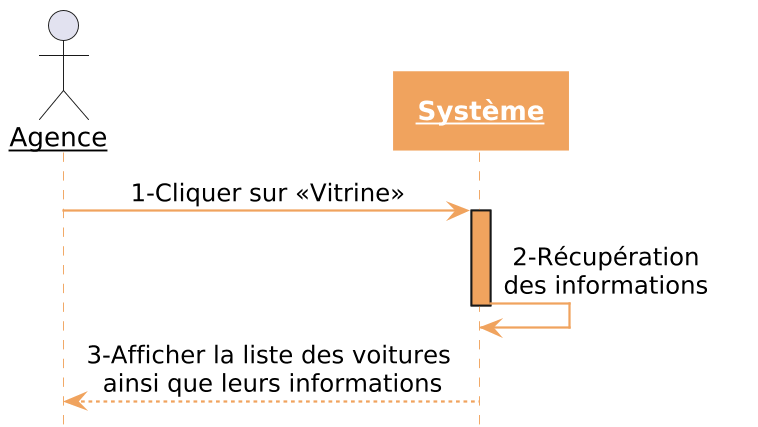
\includegraphics[width=0.7\textwidth]{Chapitres/Figures/Diag_seq_consulter_vitrine.png}
    \caption{Diagramme de séquence système de cas d'utilisation «Consulter vitrine»}
    \label{fig:consulter_vitrine}
\end{figure}
%%%%%%%%%%%%%%%%
\subsubsection{Analyse de cas d'utilisation «Modifier informations voiture»}
\label{sec:modifier_infos_voiture}
La section suivante propose une description textuelle et un diagramme de séquence, auxquels s'ajoute l'analyse du cas d'utilisation \textbf{«Modifier informations voiture»} de l'acteur \textbf{Agence}.


\begin{table}[htbp]
\centering
\caption{Description textuelle du cas d'utilisation «Modifier informations voiture»}
\label{tab:modifier_infos_voiture}
\renewcommand{\arraystretch}{1.3}
\resizebox{\textwidth}{!}{%
\begin{tabular}{|l|p{11cm}|}
\hline
\textbf{Élément} & \textbf{Description} \\
\hline
Nom & Modifier informations voiture \\
\hline
Acteur & Agence \\
\hline
Description brève & Permet à un Agence de consulter et de modifier ses informations voiture (nom, email, adresse, numéro de téléphone). \\
\hline
Précondition & 
L'agence est authentifié. \newline
Le système est accessible. \\
\hline
Postcondition & 
Les informations du voiture sont mises à jour. \newline
Les nouvelles données sont enregistrées. \\
\hline
Enchaînement principal & 
1. L'agence accède à la page «vitrine». \newline
2. Le système affiche les voiture actuelles. \newline
3. L'agence modifie les informations d'une voiture. \newline
4. Le système vérifie les données et effectue l'action. \newline
5. Le système affiche un message de confirmation. \\
\hline
\multirow{4}{*}{\textbf{Scénarios alternatifs}} 
& 4.1 Informations invalides. \\
& \quad 4.1.1 Le système affiche un message d'erreur. \\
& 5.1 Échec lors de l'enregistrement. \\
& \quad 5.1.1 Le système affiche un message d'échec. \\
\hline
\end{tabular}%
}
\end{table}
\begin{figure}[H]
    \centering
    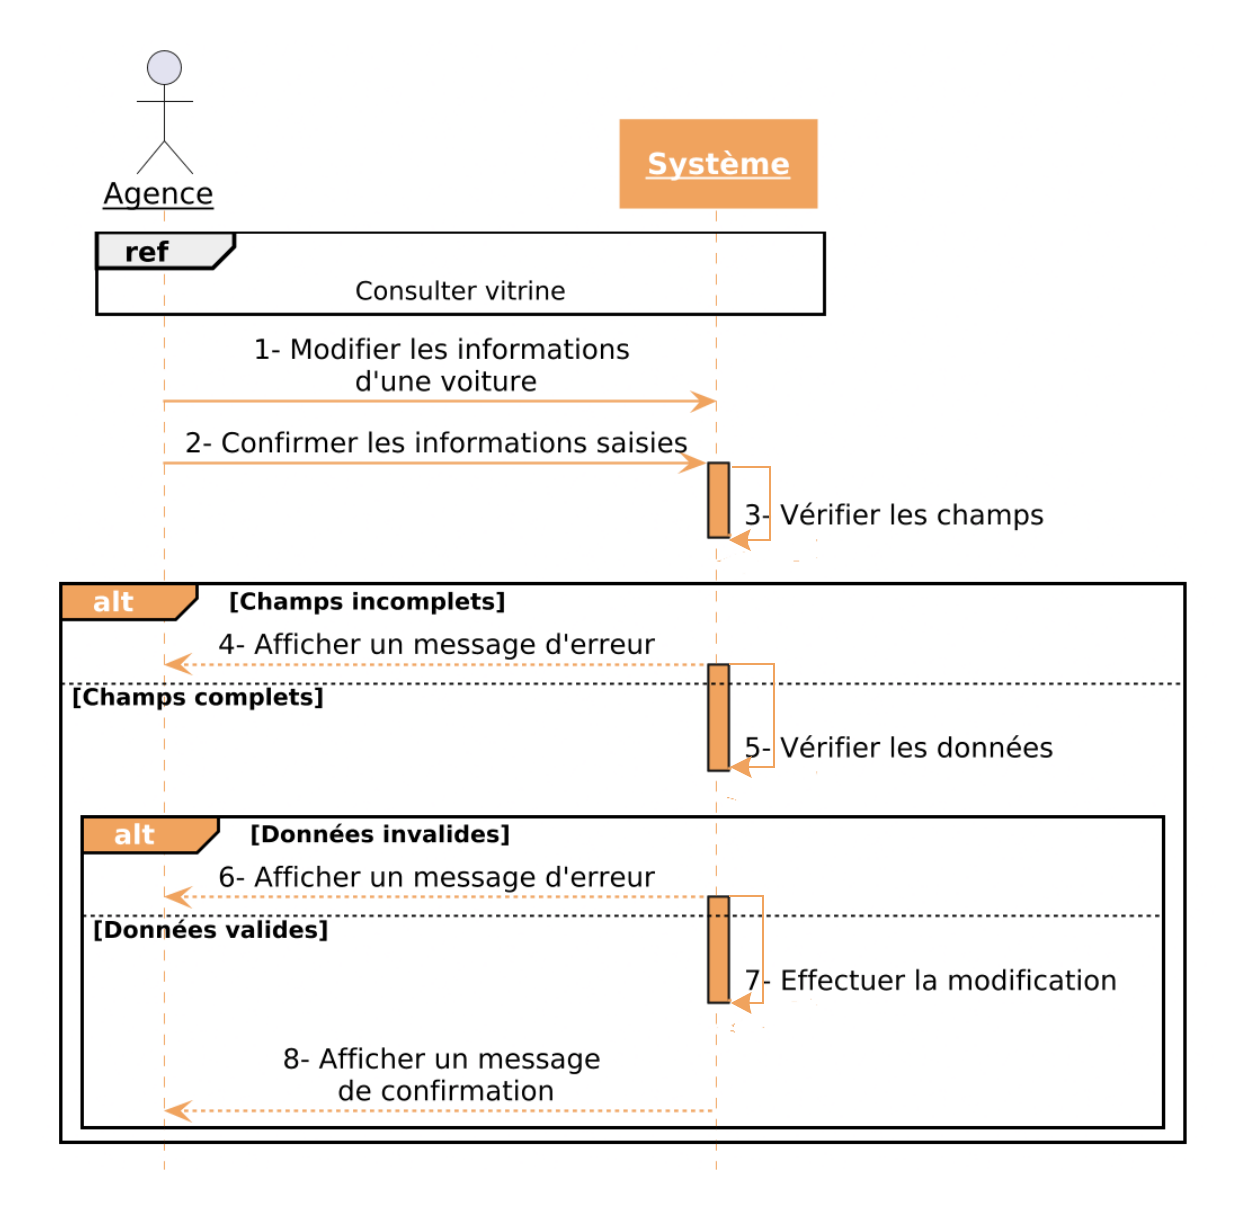
\includegraphics[width=1\textwidth]{Chapitres/Figures/Diag_seq_modifier_infos_voiture.png}
    \caption{Diagramme de séquence système de cas d'utilisation «Modifier infos voiture»}
    \label{fig:modifier_infos_voiture}
\end{figure}
%%%%%%%%%%%%%%%%%%
\subsection{Analyse de cas d'utilisation «Ajouter voiture»}
\label{sec:ajouter_voiture}
Dans la suite, nous présentons unee description textuelle accompagnée d'une diagramme 
de séquence du cas d'utilisation \textbf{«Ajouter voiture»} de l'acteur 
\textit{Agence}.

\begin{table}[H]
\centering
\caption{Description textuelle du cas d'utilisation «Ajouter voiture»}
\label{tab:ajouter_voiture}
\renewcommand{\arraystretch}{1.3}
\resizebox{\textwidth}{!}{%
\begin{tabular}{|l|p{11cm}|}
\hline
\textbf{Élément} & \textbf{Description} \\
\hline
Nom & Ajouter voiture \\
\hline
Acteur & Agence \\
\hline
Description brève & Permet à l'agence d'ajouter une voiture. \\
\hline
Précondition & 
 L'agence est authentifié. \newline
 Le système est accessible. \\
\hline
Postcondition & 
 Une voiture est ajoutée. \\
\hline
Enchaînement principal & 
1. L'agence accède à la page «Vitrine». \newline
2. Le système affiche la liste des voitures. \newline
3. L'agence choisit d'ajouter une voiture. \newline
4. L'agence saisit les informations nécessaires. \newline
5. Le système vérifie les données. \newline
6. Le système enregistre l'voiture. \newline
7. Le système affiche une message de confirmation. \\
\hline
\multirow{6}{*}{\textbf{Scénario alternatif}} & 5.1 Informations invalides.\\
& \quad 5.1.1 Le système affiche une message d'erreur. \\
& 6.1 Erreur lors de l'enregistrement. \\
& \quad 6.1.1 Le système affiche une message d'échec. \\
\hline
\end{tabular}%
}
\end{table}

\begin{figure}[H]
    \centering
    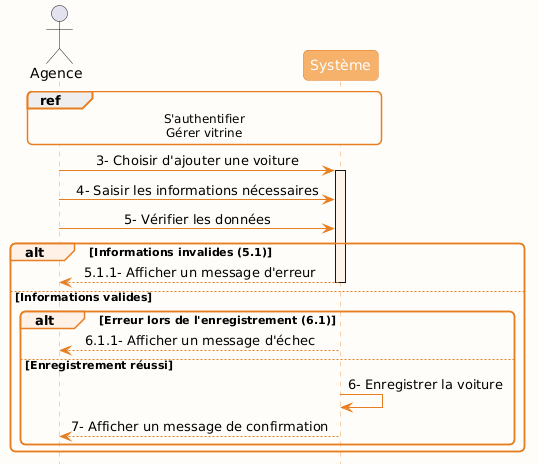
\includegraphics[width=1\textwidth]{Chapitres/Figures/Diag_seq_ajouter_voiture.png}
    \caption{Diagramme de séquence système de cas d'utilisation «Ajouter voiture»}
    \label{fig:ajouter_voiture}
\end{figure}


%%%%%%%%%%%%%%%%%%%%%%%%%%%%%%%%%%%%%%%%%%%%%%%%%%%%%%%%%%%%%%%%%%%%%%%%%%%


%%%%%%%%%%%%%%%%%%%%%%%%%
\FloatBarrier
\section{Conception des cas d'utilisation}
\label{conception_des_cas_d_utilisation}
Nous illustrerons dans cette section la conception de ce premier sprint à travers la
réalisation d'un diagramme des classes pour chaque module, ainsi que d'un diagramme
de séquence détaillé correspondant à chaque cas d'utilisation analysé
%%%%%%%%%%%%%%%%%%%%%%%%%%%%%%%%%%%%%%%%%%%%%%%%%%%%%%%%%%%%%%%%%%%%%%%%%%%
\newpage
\subsection{Diagramme des classes participantes}
\label{Diag_classes_participantes_s1}

Un diagramme des classes participantes est une représentation UML utilisée 
dans la phase d’analyse pour décrire la réalisation d’un cas d’utilisation 
spécifique. Il met en évidence les différentes classes impliquées dans 
l’interaction, ainsi que leurs responsabilités et leurs relations, afin de 
structurer le comportement du système selon une approche orientée objet.\cite{stackoverflow}

Ce diagramme repose généralement sur trois catégories principales de classes d’analyse :

\begin{enumerate}
    \item \textbf{Les classes frontières (ou classes de dialogue)} : 
    Elles assurent l’interaction entre l’utilisateur et le système. 
    Elles contiennent des attributs correspondant aux données affichées ou saisies 
    (champs de formulaires, résultats, etc.) et des opérations représentant 
    les actions effectuées par l’utilisateur via l’interface homme-machine (IHM).\cite{stackoverflow}

    \item \textbf{Les classes de contrôle} : 
    Elles orchestrent le déroulement du cas d’utilisation. 
    Elles implémentent la logique applicative, coordonnent les échanges entre 
    les classes frontières et les classes entités, et encapsulent les règles 
    métier ainsi que les traitements du système.\cite{stackoverflow}

    \item \textbf{Les classes entités} : 
    Elles représentent les données métier du système. 
    Ces classes contiennent des attributs persistants correspondant aux informations 
    stockées (par exemple dans une base de données) et peuvent inclure des opérations 
    liées à la gestion de ces données.\cite{stackoverflow}
\end{enumerate}

\subsubsection{Diagramme des classes participantes par acteur «Internaute»}
\label{Diag_classes_participantes_internaute_s1}
\begin{figure}[H]
    \centering
    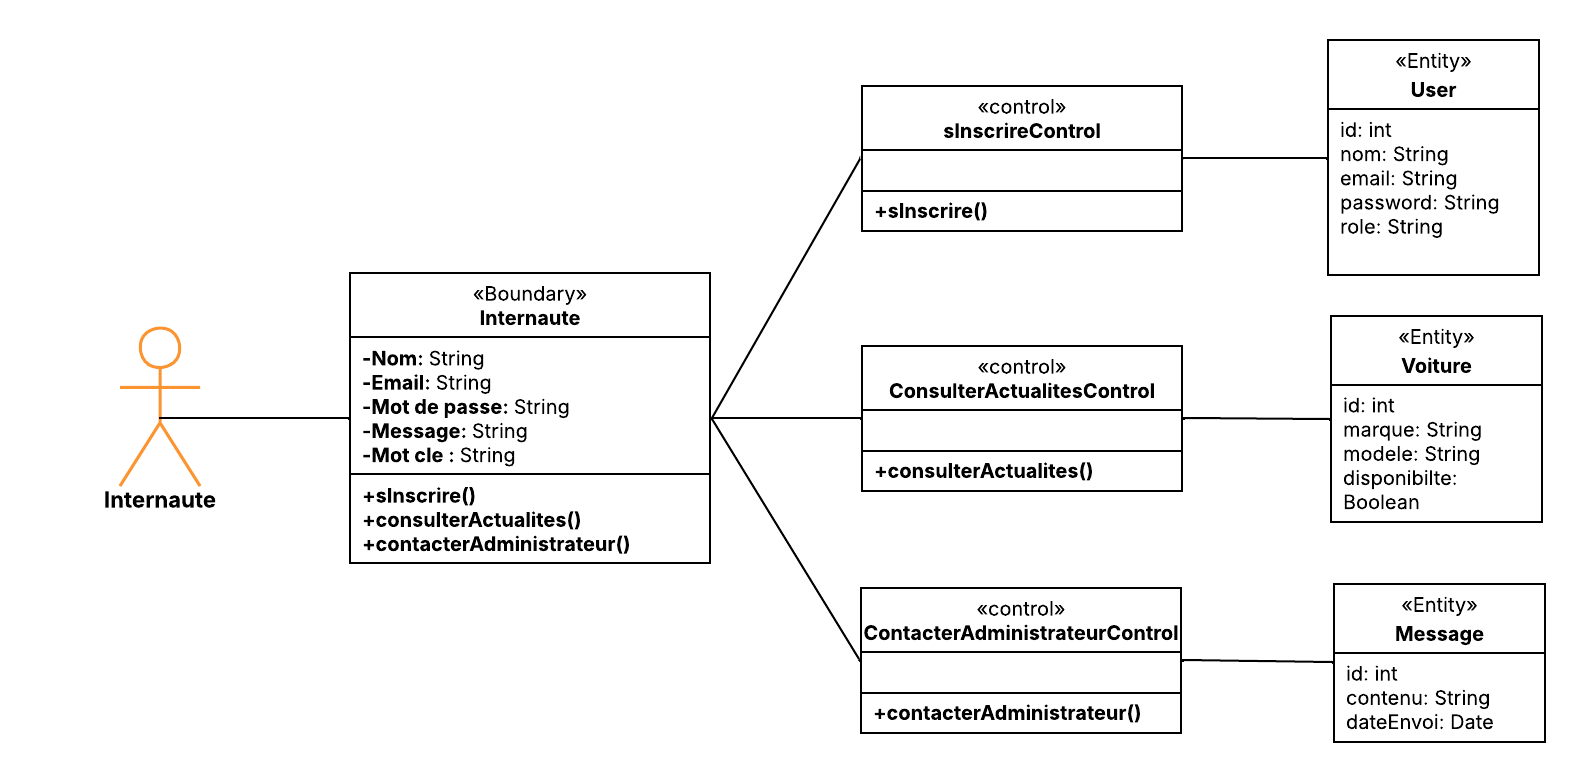
\includegraphics[width=1\textwidth]{Chapitres/Figures/classes_participantes__internaute_s1.png}
    \caption{Diagramme des classes participantes par acteur Internaute}
    \label{fig:classes_participantes_internaute_s1}
\end{figure}

\subsubsection{Diagramme des classes participantes par acteur «Utilisateur»}
\label{Diag_classes_participantes_utilisateur_s1}
\begin{figure}[H]
    \centering
    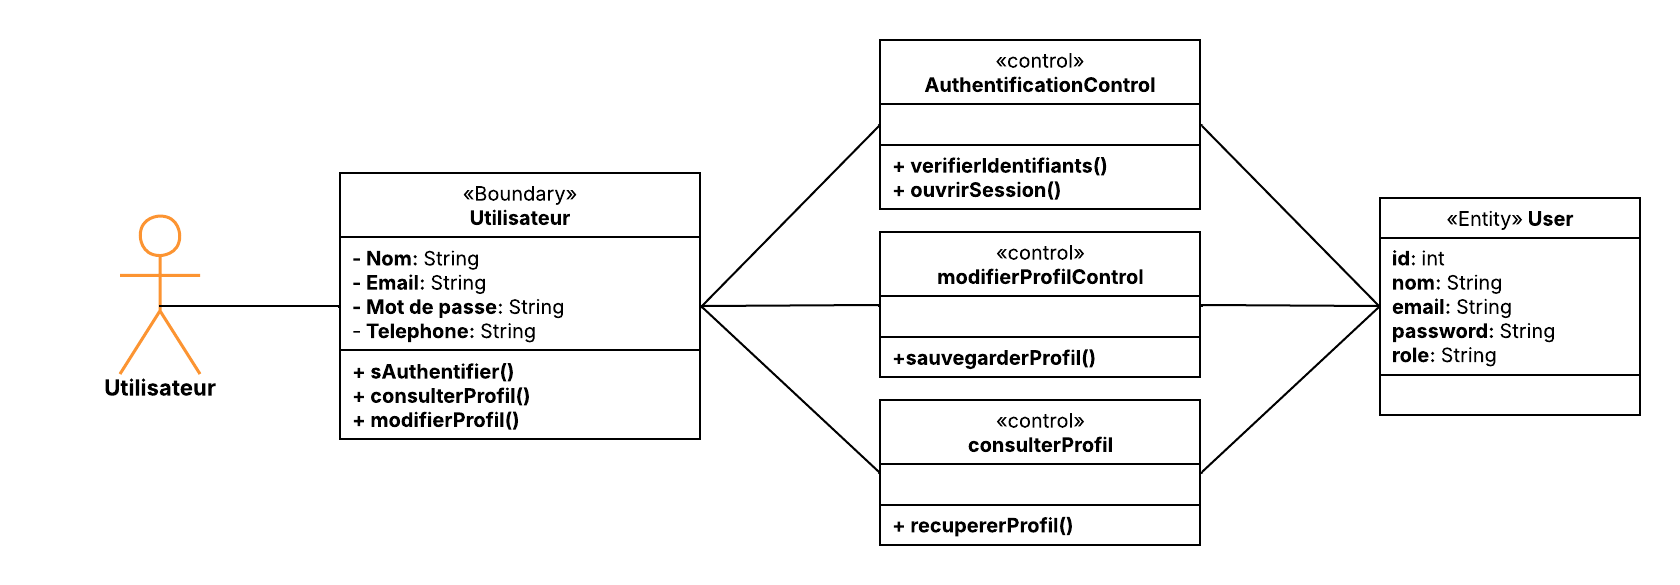
\includegraphics[width=1\textwidth]{Chapitres/Figures/classes_participantes__utilisateur_s1.png}
    \caption{Diagramme des classes participantes par acteur Utilisateur}
    \label{fig:classes_participantes_utilisateur_s1}
\end{figure}

\subsubsection{Diagramme des classes participantes par acteur «Agence»}
\label{Diag_classes_participantes_agence_s1}
\begin{figure}[H]
    \centering
    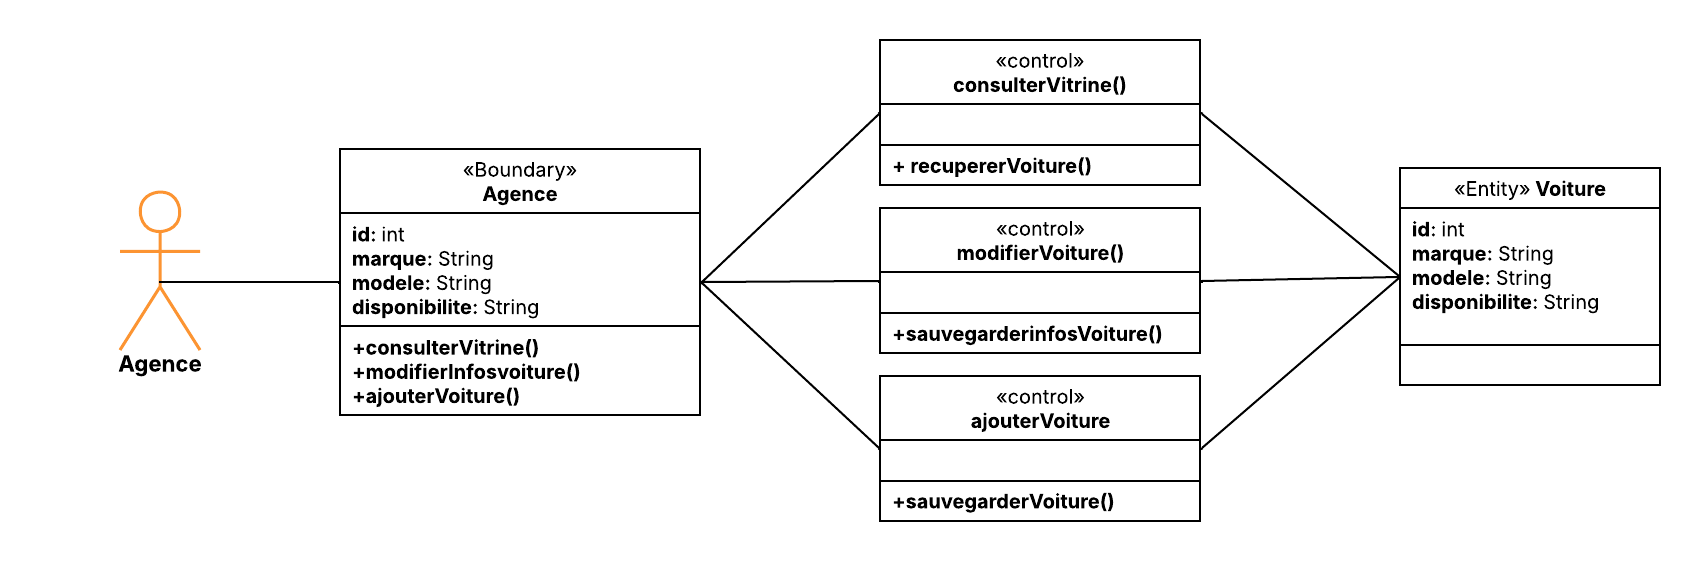
\includegraphics[width=1\textwidth]{Chapitres/Figures/classes_participantes__agence_s1.png}
    \caption{Diagramme des classes participantes par acteur Agence}
    \label{fig:classes_participantes_agence_s1}
\end{figure}

\subsubsection{Diagramme des classes participantes par acteur «Administrateur»}
\label{Diag_classes_participantes_administrateur_s1}
\begin{figure}[H]
    \centering
    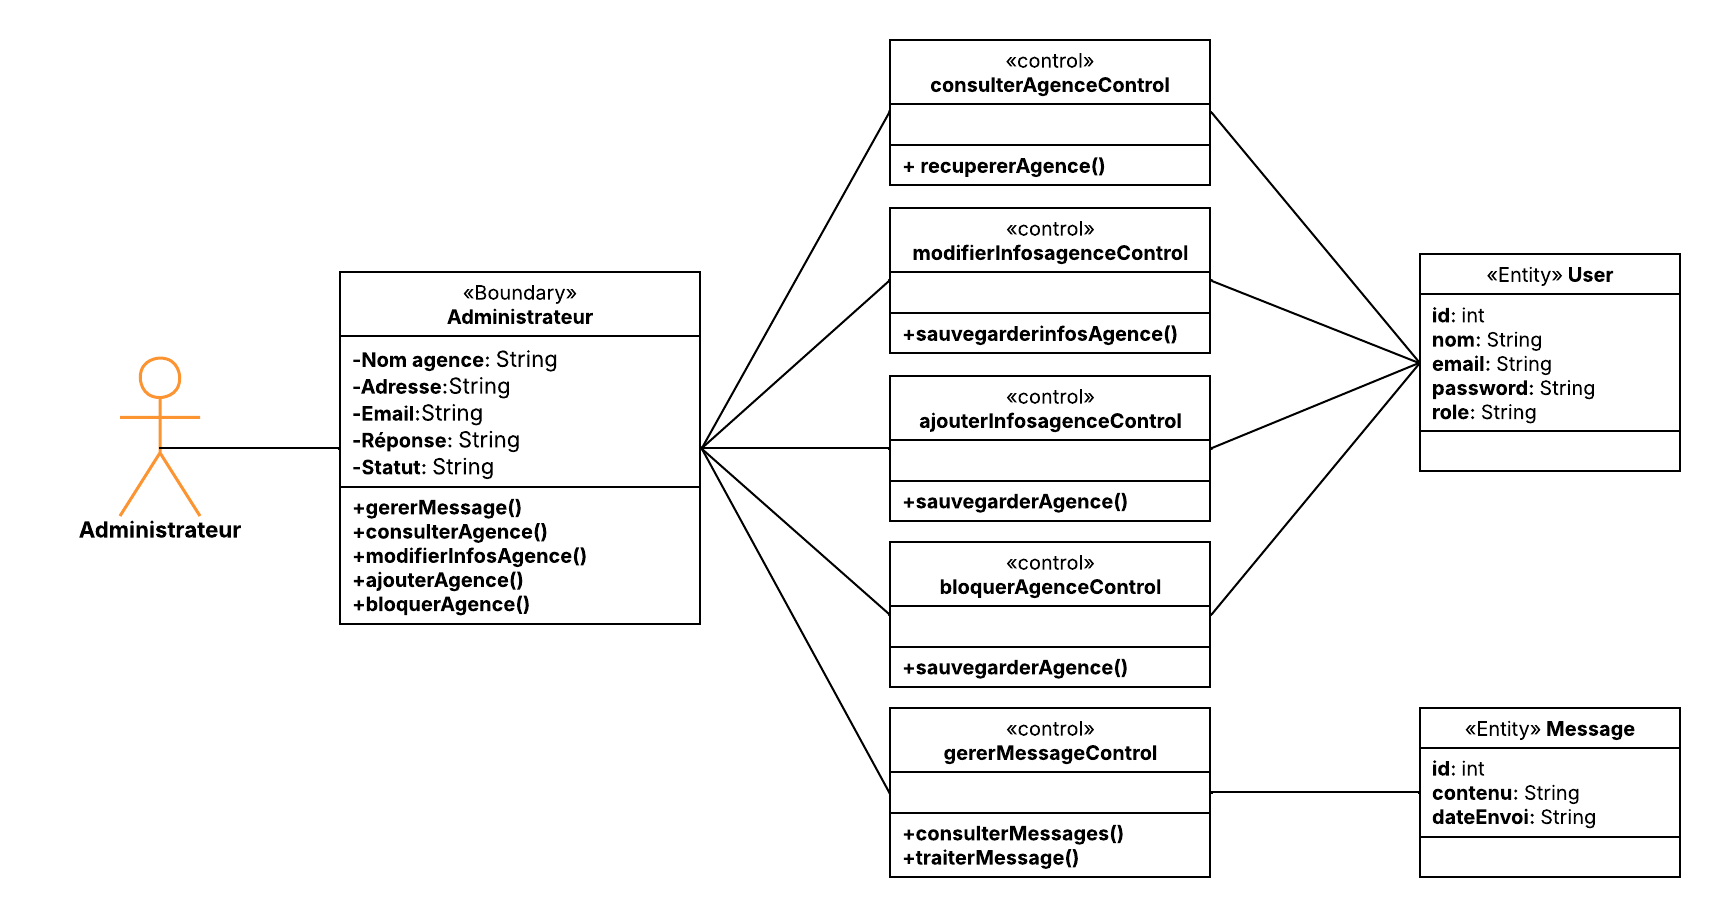
\includegraphics[width=1\textwidth]{Chapitres/Figures/classes_participantes__admin_s1.png}
    \caption{Diagramme des classes participantes par acteur Administrateur}
    \label{fig:classes_participantes_admin_s1}
\end{figure}

%%%%%%%%%%%seq_détaillé%%%%%%%%%%%%%%%%%%%%%%%%%%%%%%%%%%%%%%%%%%%%%%%%%%%%%%%%%%%%%%%%%%%%%%%%%%%%%%%%%%%%%
\section{Diagrammes de séquence détaillés du premier sprint}
\label{sec:diag_seq_detail_s1}
\textit{"Les diagrammes de séquence sont un outil essentiel en génie logiciel pour visualiser les interactions entre les objets d’un système au fil du temps. Ils aident à comprendre le comportement dynamique d’un système, à concevoir son architecture et à documenter des processus complexes. Ce guide couvrira les concepts clés, les recommandations, un exemple concret et une étude de cas pour vous aider à maîtriser les diagrammes de séquence.''}\cite{cybermedian}


%====================================================x²
\subsection{Diagrammes de séquence détaillés de l’acteur Internaute}
\label{sec:diag_seq_internaute}

\subsubsection{Diagrammes de séquence détaillé du cas d’utilisation « Consulter actualités »}
\label{sec:diag_seq_det_consulter_actualite}
\begin{figure}[H]
    \centering
    
\includegraphics[width=0.8\textwidth]{Chapitres/figures/diag_seq_det/seq_det_s1/seq_det_consulter_actualite.png}
    \caption{Diagramme de séquence détaillé du cas d’utilisation « Consulter actualités »}
    \label{fig:seq_det_consulter_actualite}
\end{figure}

\subsubsection{Diagrammes de séquence détaillé du cas d’utilisation « S’inscrire »}
\label{sec:diag_seq_det_s_inscrire}
\begin{figure}[H]
    \centering
    
\includegraphics[width=0.95\textwidth]{Chapitres/figures/diag_seq_det/seq_det_s1/seq_det_s_inscrire.png}
    \caption{Diagramme de séquence détaillé du cas d’utilisation « S’inscrire »}
    \label{fig:seq_det_s_inscrire}
\end{figure}

%====================================================
\subsection{Diagrammes de séquence détaillés de l’acteur Utilisateur}
\label{sec:diag_seq_utilisateur}


\subsubsection{Diagrammes de séquence détaillé du cas d’utilisation « S’authentifier »}
\label{sec:diag_seq_det_s_authentifier}
\begin{figure}[H]
    \centering
    
\includegraphics[width=0.85\textwidth]{Chapitres/figures/diag_seq_det/seq_det_s1/seq_det_s_authentifier.png}
    \caption{Diagramme de séquence détaillé du cas d’utilisation « S’authentifier »}
    \label{fig:seq_det_s_authentifier}
\end{figure}


\subsubsection{Diagrammes de séquence détaillé du cas d’utilisation « Interagir avec Chatbot »}
\label{sec:diag_seq_det_chatbot}
\begin{figure}[H]
    \centering
    
\includegraphics[width=0.85\textwidth]{Chapitres/figures/diag_seq_det/seq_det_s1/seq_det_chatbot.png}
    \caption{Diagramme de séquence détaillé du cas d’utilisation « Interagir avec Chatbot »}
    \label{fig:seq_det_chatbot}
\end{figure}

\subsubsection{Diagrammes de séquence détaillé du cas d’utilisation « Consulter profil »}
\label{sec:diag_seq_det_consulter_profil}
\begin{figure}[H]
    \centering
    
\includegraphics[width=0.85\textwidth]{Chapitres/figures/diag_seq_det/seq_det_s1/seq_det_consulter_profil.png}
    \caption{Diagramme de séquence détaillé du cas d’utilisation « Consulter profil »}
    \label{fig:seq_det_consulter_profil}
\end{figure}

%====================================================
\subsection{Diagrammes de séquence détaillés de l’acteur Administrateur}
\label{sec:diag_seq_admin_s1}

\subsubsection{Diagrammes de séquence détaillé du cas d’utilisation « Ajouter agence »}
\label{sec:diag_seq_det_ajouter_agence}
\begin{figure}[H]
    \centering
    
\includegraphics[width=0.8\textwidth]{Chapitres/figures/diag_seq_det/seq_det_s1/seq_det_ajouter_agence.png}
    \caption{Diagramme de séquence détaillé du cas d’utilisation « Ajouter agence »}
    \label{fig:seq_det_ajouter_agence}
\end{figure}

\subsubsection{Diagrammes de séquence détaillé du cas d’utilisation « Bloquer/Débloquer agence »}
\label{sec:sec_diag_seq_det_bloquer_agence}
\begin{figure}[H]
    \centering
    
\includegraphics[width=0.8\textwidth]{Chapitres/figures/diag_seq_det/seq_det_s1/seq_det_bloquer_agence.png}
    \caption{Diagramme de séquence détaillé du cas d’utilisation « Bloquer/Débloquer agence »}
    \label{fig:seq_det_bloquer_agence}
\end{figure}

\subsubsection{Diagrammes de séquence détaillé du cas d’utilisation « Ajouter utilisateur »}
\label{sec:diag_seq_det_ajouter_utilisateur}
\begin{figure}[H]
    \centering
    
\includegraphics[width=0.8\textwidth]{Chapitres/figures/diag_seq_det/seq_det_s1/seq_det_ajouter_utilisateur.png}
    \caption{Diagramme de séquence détaillé du cas d’utilisation « Ajouter utilisateur »}
    \label{fig:seq_det_ajouter_utilisateur}
\end{figure}

\subsubsection{Diagrammes de séquence détaillé du cas d’utilisation « Bloquer/Débloquer utilisateur »}
\label{sec:diag_seq_det_bloquer_agence}
\begin{figure}[H]
    \centering
    
\includegraphics[width=0.8\textwidth]{Chapitres/figures/diag_seq_det/seq_det_s1/seq_det_bloquer_utilisateur.png}
    \caption{Diagramme de séquence détaillé du cas d’utilisation « Bloquer/Débloquer utilisateur »}
    \label{fig:seq_det_bloquer_utilisateur}
\end{figure}

\newpage
\FloatBarrier
\section{Diagramme de classe du premier sprint}
\label{section3.diag_classes}
Un diagramme de classes est une représentation graphique qui identifie les principales classes d’un système, leurs attributs, leurs méthodes et les relations qui les lient. Chaque classe est figurée par un rectangle divisé en trois parties (nom, attributs, opérations), et les liens entre classes traduisent des relations comme l’héritage, l’association ou la dépendance. Ce type de diagramme permet de structurer et de visualiser l’architecture logicielle, en offrant une vue claire des entités et de leurs interactions essentielles.\cite{Lucidchart}
%%%%%%%%%%%%%%%%%%%%%%%%%%%%%%%%%%%%%%%%%%%%%%%%%%%%%%%%%%%%%%%%%%%%%%%%%%%

\begin{figure}[H]
    \centering
    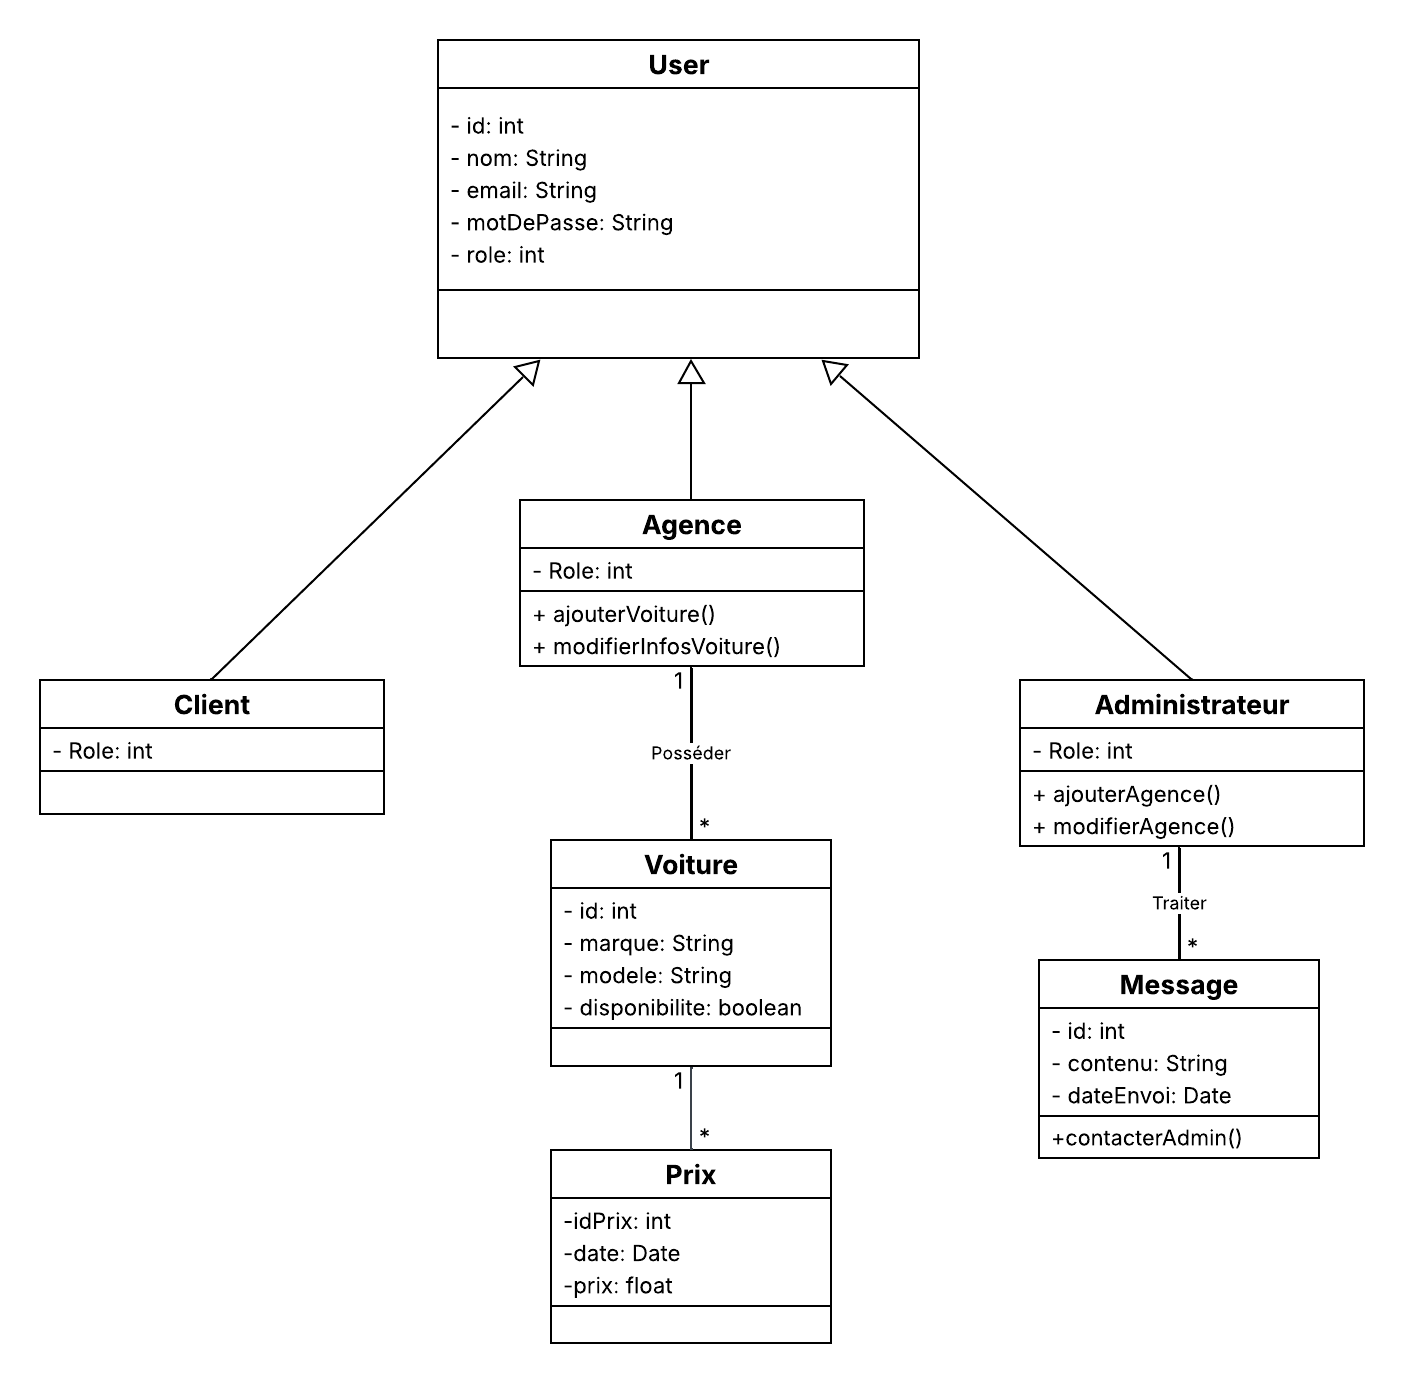
\includegraphics[width=1\textwidth]{Chapitres/Figures/Diag_classe_sprint_1.png}
    \caption{Diagramme de classe du premier sprint}
    \label{fig:diag_classes}
\end{figure}
%%%%%%%%%%%%%%%%%%%%%%%%%%%%%%%%%%%%%%%%%%%%%%%%%%%%%%%%%%%%%%%%%%%%%%%%%%%%%%%%%%%%%%%%%%%%%%%%%%%%%%%%%%%%
\section{Implémentation}
\label{sec:implementation_s1}

Le module d'implémentation d'un projet prévoit l'implémentation des fonctions qui ont été réalisées au cours du premier sprint.

\subsection{Tables de la base de données}

Le tableau ci-joint décrit le répertoire de données afin d'illustrer les attributs que l'on retrouve dans les différentes classes, ainsi que leurs étiquettes et leurs types.

\subsubsection{Tableau « users »}

\begin{table}[H]
\centering
\caption{Tableau « users »}
\label{tab:users}
\renewcommand{\arraystretch}{1.3}
\resizebox{\textwidth}{!}{%
\begin{tabular}{|l|l|p{4cm}|l|}
\hline
\textbf{Champs} & \textbf{Type} & \textbf{Libellé} & \textbf{Contraintes} \\
\hline
id & Int & Identifiant unique de l'utilisateur & PRIMARY KEY, NOT NULL \\
\hline
name & String & Le nom de l'utilisateur & NOT NULL \\
\hline
email & String & L'email de l'utilisateur & NOT NULL, UNIQUE \\
\hline
email\_verified\_at & Timestamp & La date de vérification de l'email & NULLABLE \\
\hline
password & String & Le mot de passe de l'utilisateur & NOT NULL \\
\hline
must\_change\_password & Tinyint(1) & Indique si l'utilisateur doit changer son mot de passe & NOT NULL, DEFAULT 0 \\
\hline
role & Enum & Le rôle de l'utilisateur (client / agency\_admin / super\_admin) & NOT NULL \\
\hline
agency\_id & BigInt & Identifiant unique de l'agence & FOREIGN KEY, NULLABLE \\
\hline
phone & String & Le numéro de téléphone de l'utilisateur & NULLABLE \\
\hline
address & Text & L'adresse de l'utilisateur & NULLABLE \\
\hline
driver\_license & String & Le permis de conduire de l'utilisateur & NULLABLE \\
\hline
is\_suspended & Boolean & Indique si l'utilisateur est suspendu & NOT NULL, DEFAULT 0 \\
\hline
suspension\_reason & Text & La raison de la suspension de l'utilisateur & NULLABLE \\
\hline
suspended\_at & Timestamp & La date de suspension de l'utilisateur & NULLABLE \\
\hline
remember\_token & String & Token de mémorisation & NULLABLE \\
\hline
created\_at & Timestamp & Date de création & NOT NULL \\
\hline
updated\_at & Timestamp & Date de modification & NOT NULL \\
\hline
\end{tabular}%
}
\end{table}

\subsubsection{Tableau « vehicles »}

\begin{table}[H]
\centering
\caption{Tableau « vehicles »}
\label{tab:vehicles}
\renewcommand{\arraystretch}{1.3}
\resizebox{\textwidth}{!}{%
\begin{tabular}{|l|l|p{4cm}|l|}
\hline
\textbf{Champs} & \textbf{Type} & \textbf{Libellé} & \textbf{Contraintes} \\
\hline
id & Int & Identifiant unique du véhicule & PRIMARY KEY, NOT NULL \\
\hline
brand & String & La marque du véhicule & NOT NULL \\
\hline
model & String & Le modèle du véhicule & NOT NULL \\
\hline
year & Int & L'année du véhicule & NOT NULL \\
\hline
mileage & Int & Le kilométrage du véhicule & NOT NULL \\
\hline
daily\_price & Decimal(8,2) & Le prix journalier de location & NOT NULL \\
\hline
caution\_amount & Decimal(10,2) & Le montant de la caution fixé par l'agence & NULLABLE \\
\hline
license\_plate & String & La plaque d'immatriculation & NOT NULL, UNIQUE \\
\hline
color & String & La couleur du véhicule & NOT NULL \\
\hline
seats & Int & Le nombre de places & NOT NULL \\
\hline
transmission & Enum & Le type de transmission (manual / automatic) & NOT NULL \\
\hline
fuel\_type & Enum & Le type de carburant (petrol / diesel / electric / hybrid) & NOT NULL \\
\hline
status & Enum & L'état du véhicule (available / reserved / in\_use / returned) & NOT NULL, DEFAULT available \\
\hline
agency\_id & BigInt UNSIGNED & Identifiant unique de l'agence & FOREIGN KEY, NOT NULL \\
\hline
created\_at & Timestamp & Date de création & NULLABLE \\
\hline
updated\_at & Timestamp & Date de modification & NULLABLE \\
\hline
images & Text & Les images du véhicule & NULLABLE \\
\hline
\end{tabular}%
}
\end{table}

\subsection{Réalisation des interfaces du premier sprint}

Nous présentons dans cette section les interfaces graphiques développées lors du premier sprint.

\subsubsection{Interface d'inscription :}

\begin{figure}[H]
    \centering
    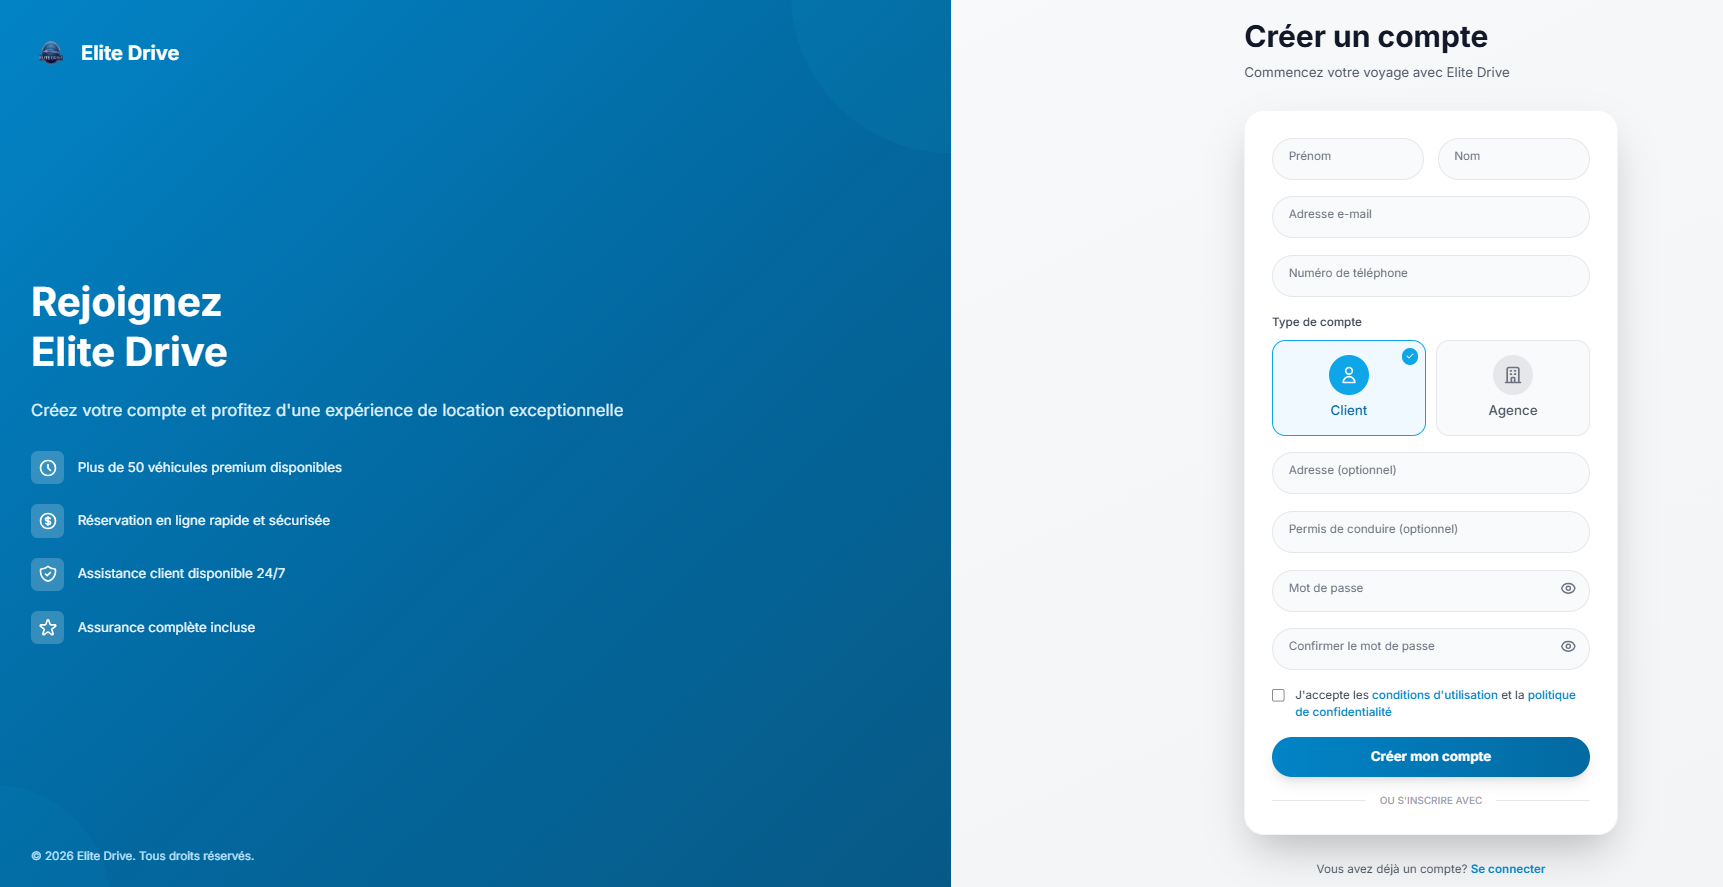
\includegraphics[width=0.9\linewidth]{Chapitres/Figures/inter_inscrire.png}
    \caption{Interface d'inscription}
    \label{fig:interface_inscription_s1}
\end{figure}

\subsubsection{Interface d'authentication :}

\begin{figure}[H]
    \centering
    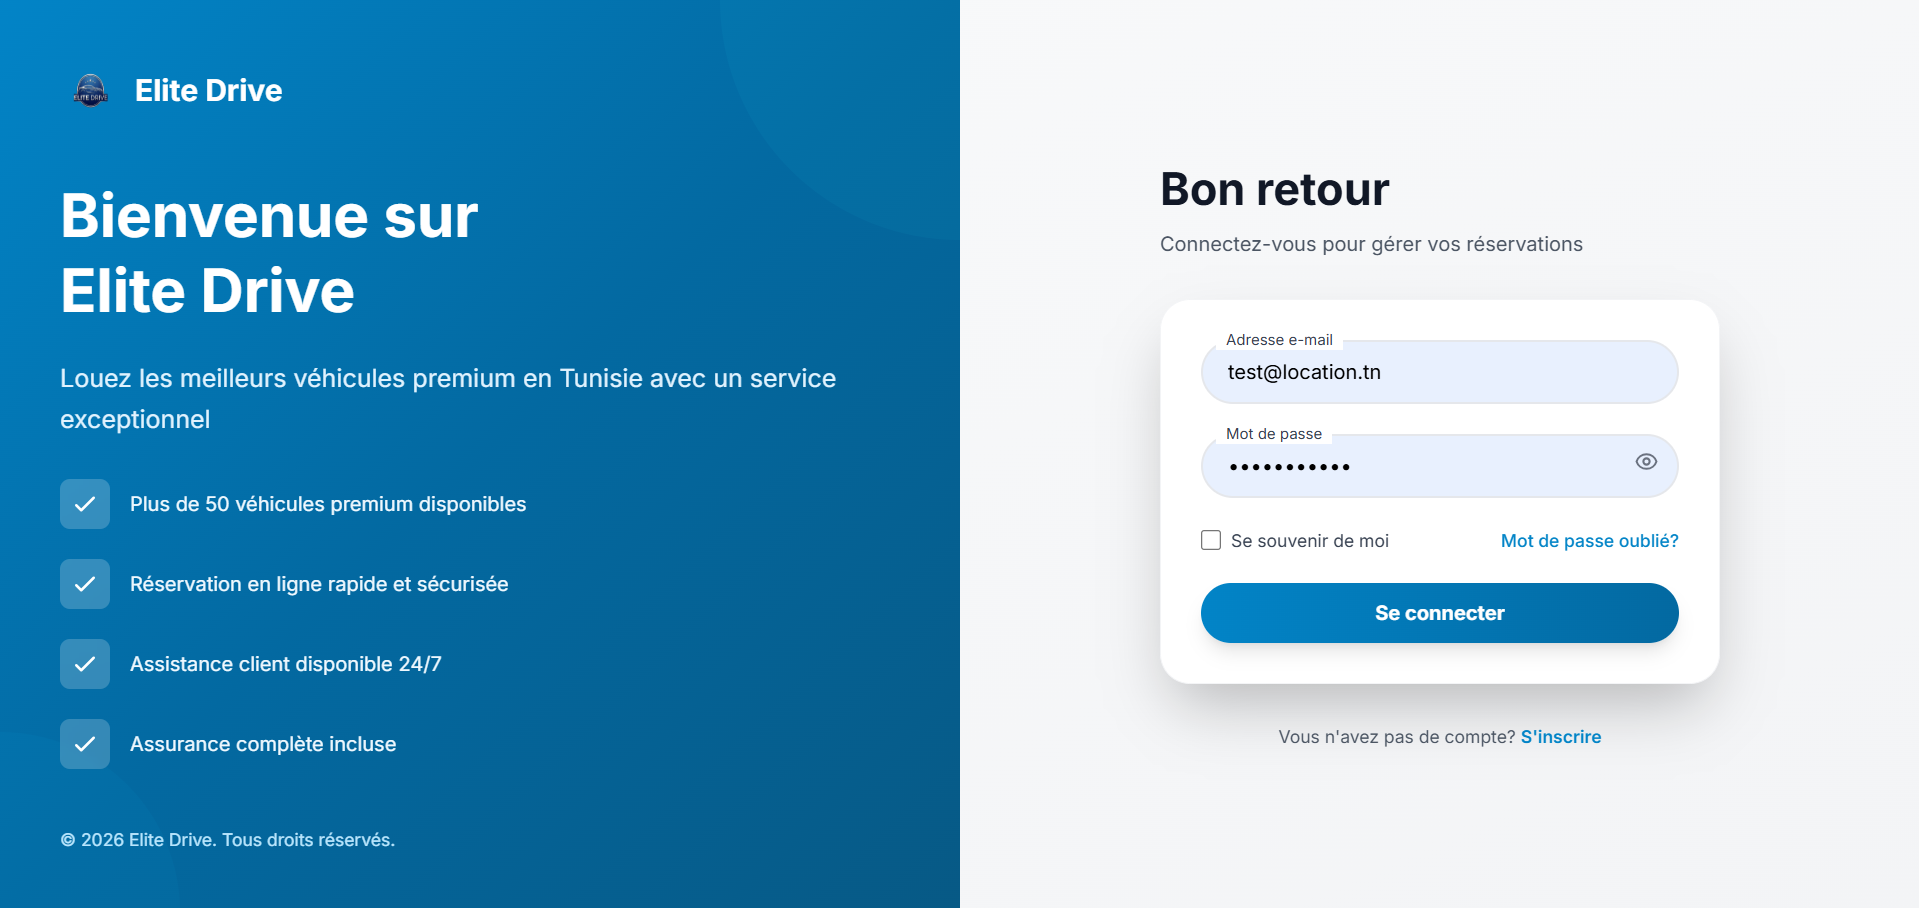
\includegraphics[width=0.9\linewidth]{Chapitres/Figures/inter_auth.png}
    \caption{Interface d'authentification}
    \label{fig:interface_authentification_s1}
\end{figure}

\subsubsection{Interface profil :}

\begin{figure}[H]
    \centering
    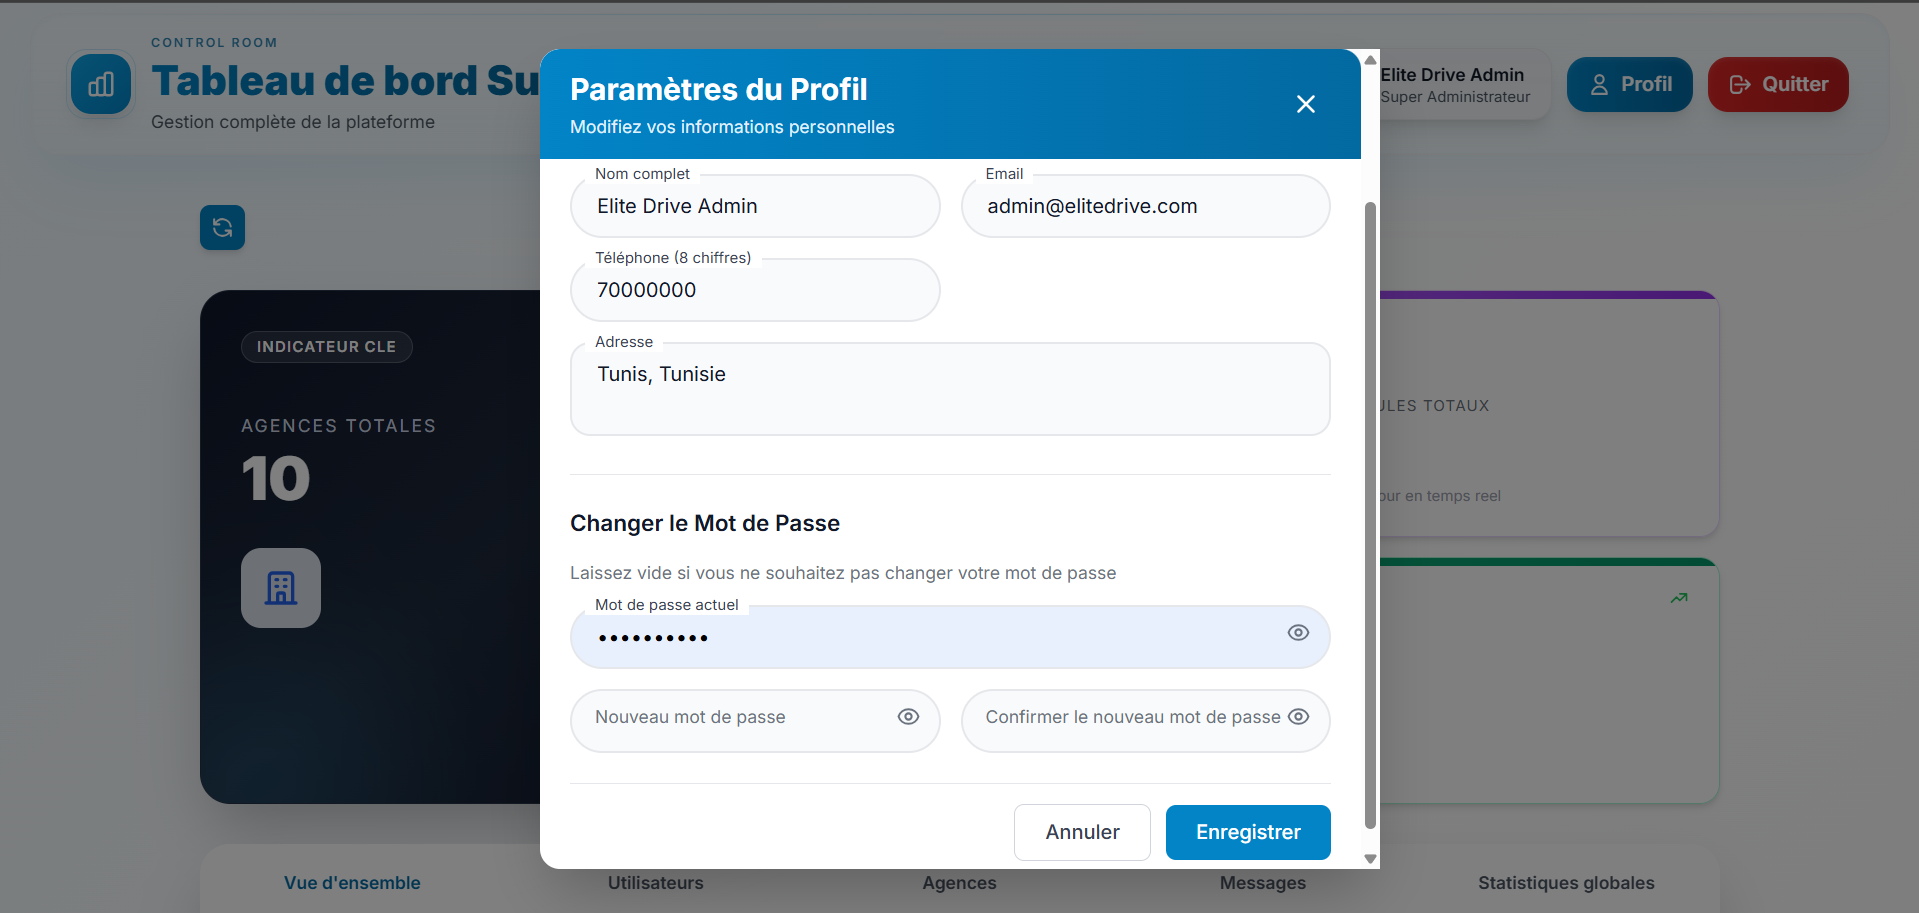
\includegraphics[width=0.9\linewidth]{Chapitres/Figures/inter_profil.png}
    \caption{Interface profil}
    \label{fig:interface_profil_s1}
\end{figure}

\subsubsection{Interface chatbot :}

\begin{figure}[H]
    \centering
    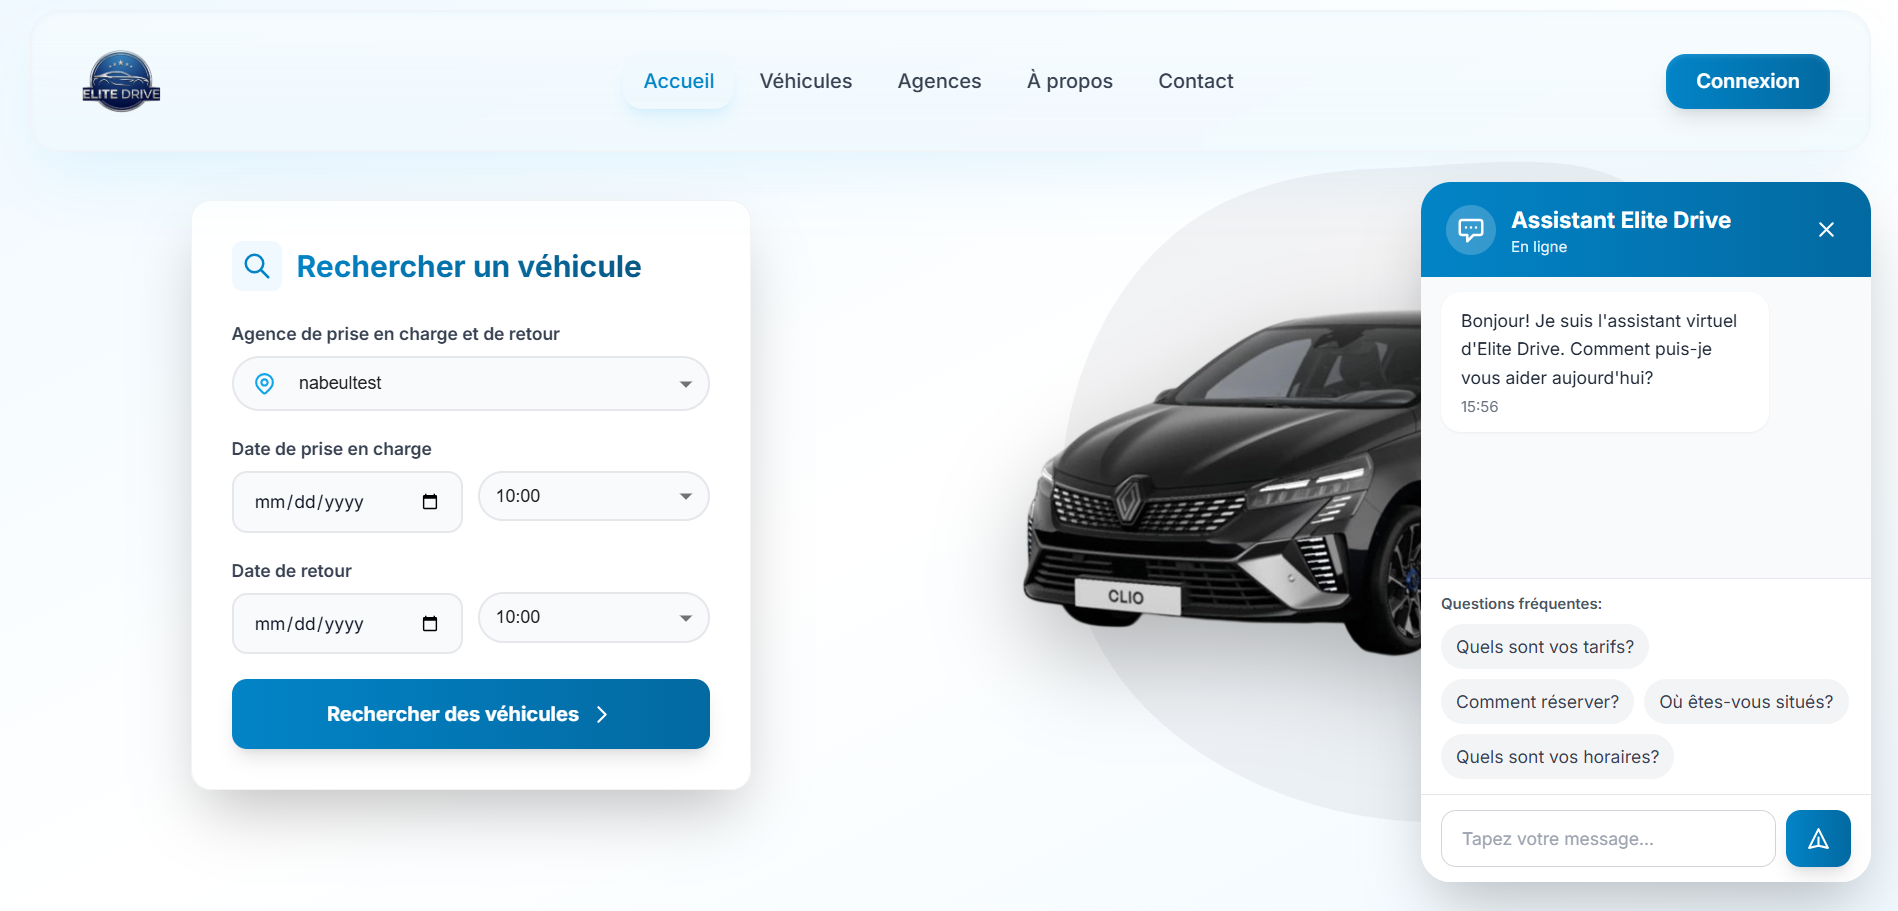
\includegraphics[width=0.9\linewidth]{Chapitres/Figures/inter_chatbot.png}
    \caption{Interface chatbot}
    \label{fig:interface_chatbot_s1}
\end{figure}

\subsubsection{Interface vitrine :}

\begin{figure}[H]
    \centering
    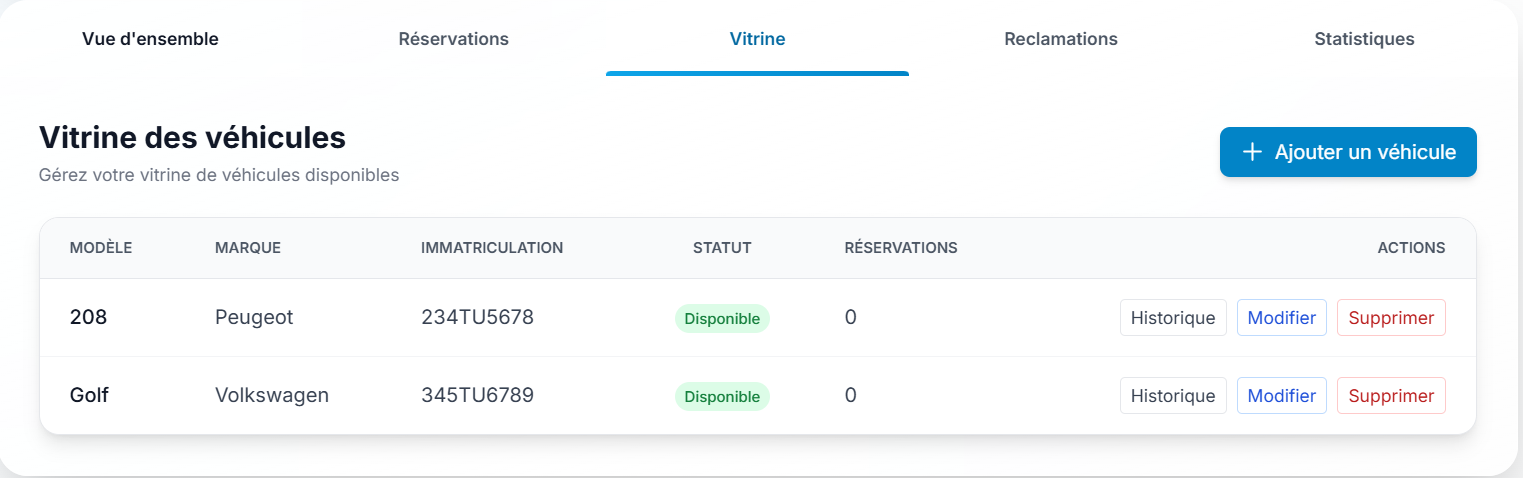
\includegraphics[width=0.9\linewidth]{Chapitres/Figures/inter_vitrine.png}
    \caption{Interface vitrine}
    \label{fig:interface_vitrine_s1}
\end{figure}

\subsubsection{Interface bloquer/debloquer une agence :}

\begin{figure}[H]
    \centering
    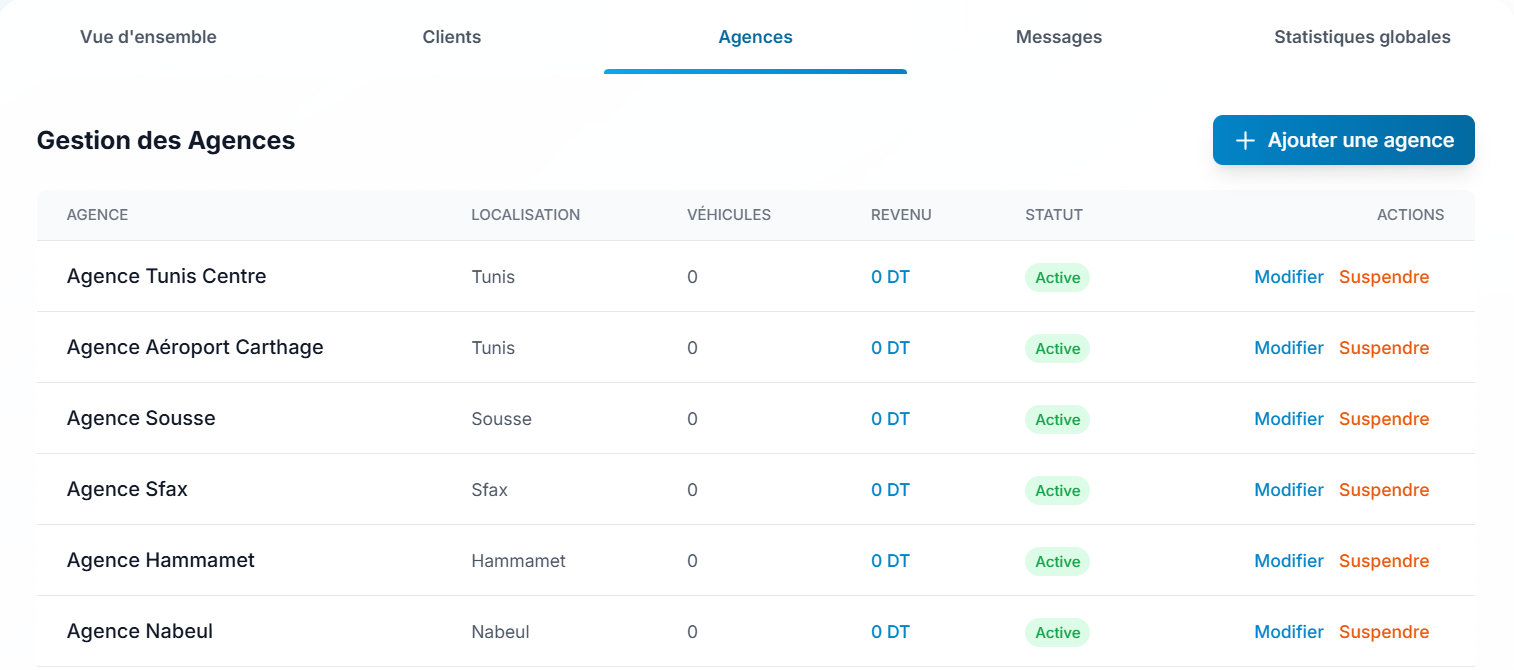
\includegraphics[width=0.9\linewidth]{Chapitres/Figures/inter_bloqAgence.png}
    \caption{Interface bloquer/débloquer une agence}
    \label{fig:interface_bloquer_debloquer_agence_s1}
\end{figure}

%%%%%%%%%%%%%%%%%%%%%%%%%%%%%%%%%%%%%%%%%%%%%%%%%%%%%%%%%%%%%%%%%%%%%%%%%%%%%%%%%%%%%%%%%%%%%%%%%%%%%%%%%%%%
\section{Test unitaire}
\subsection{Test unitaire du cas d’utilisation «S’authentifier»}

Cette section se concentre sur la récupération du code pour le cas «S’authentifier».

\subsection*{— Code source de la méthode d’authentification :}

\begin{figure}[H]
    \centering
    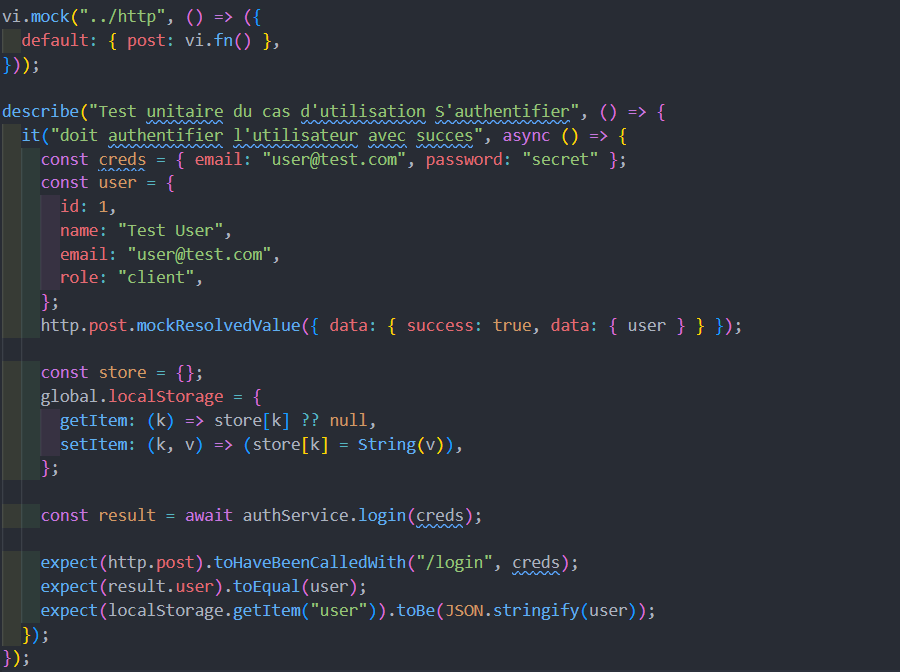
\includegraphics[width=0.9\linewidth]{Chapitres/Figures/test1_code.png}
    \caption{Test unitaire du cas d’utilisation «S’authentifier»}
\end{figure}


\subsection{Test unitaire du cas d’utilisation «Bloquer ou Débloquer une agence»}

Cette section se concentre sur la récupération du code pour le cas Bloquer ou
Débloquer une agence.

\subsection*{- Code source de la méthode de blocage ou déblocage d'une agence :}

\begin{figure}[H]
    \centering
    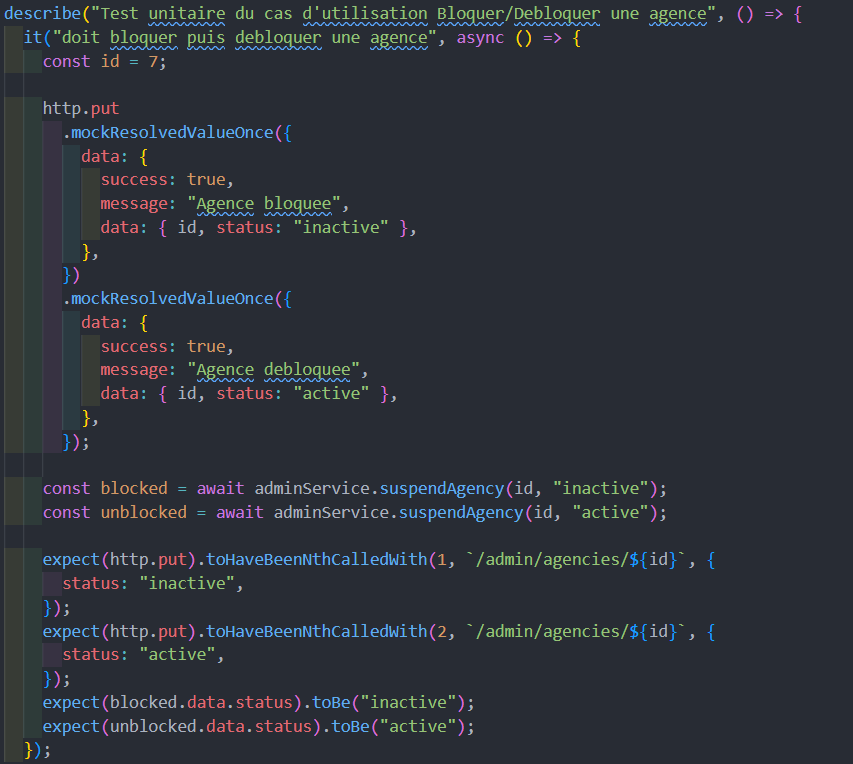
\includegraphics[width=0.9\linewidth]{Chapitres/Figures/test2_code.png}
    \caption{Test unitaire du cas d’utilisation «Bloquer ou Débloquer un agence»}
\end{figure}




%%%%%%%%%%%%%%%%%%%%%%%%%%%%%%%%%%%%%%%%%%%%%%%%%%%%%%%%%%%%%%%%%%%%%%%%%%%%%%%%%%%%%%%%%%%%%%%%%%%%%%%%%%%%
\section{Conclusion}
%%%%%%%%%%%%%%%%%%%%%%%%%%%%%%%%%%%%%%%%%%%%%%%%%%%%%%%%%%%%%%%%%%%%%%%%%%%

Dans le cadre de ce chapitre, nous avons mené le Sprint 1 selon une séquence logique couvrant l'analyse des cas d'utilisation, la conception et les tests. La phase suivante concerne la mise en œuvre du Sprint 2, qui est dédié à la gestion des réservations, des réclamations et du tableau de bord.
%==========================================================
%  CHAPITRE 4 — Réalisation du deuxième sprint
%==========================================================
\chapter{Réalisation du deuxième sprint}
\label{Chapitre_4}

{\Large\textbf{Sprint : Gérer les processus des réservations}}

%----------------------------------------------------------
\section{Introduction}
\label{Chapitre4_Introduction}

En se basant sur la planification établie dans le chapitre précédent, ce chapitre est
consacré à la réalisation du Sprint 2. Nous aborderons successivement la description
fonctionnelle, la conception, ainsi que les diagrammes de séquence et de classe
associés aux fonctionnalités développées au cours de ce sprint. Ces fonctionnalités
concernent principalement la gestion des réservations, le suivi du score client, le
traitement des réclamations, la consultation des statistiques et la gestion des messages.

%----------------------------------------------------------
\section{Backlog produit du deuxième sprint}
\label{sec:backlog_sprint2}

\begin{table}[H]
\centering
\caption{Backlog produit du deuxième sprint}
\label{tab:backlog-sprint2}
\renewcommand{\arraystretch}{1.4}
\resizebox{\textwidth}{!}{
\begin{tabular}{|l|c|l|p{4cm}|p{5cm}|c|}
\hline
\textbf{Acteur} & \textbf{ID} & \textbf{Thème} & \textbf{User Story} & \textbf{Tâche} & \textbf{Estimation (Jours)} \\
\hline

\multirow{2}{*}{Internaute}
& US15 & Interagir avec chatbot 
& Interagir avec le chatbot
& Intégrer le module chatbot. & \multirow{2}{*}{4} \\
\cline{5-5}
& & & & Tester. & \\
\hline

\multirow{4}{*}{Client}
& US09 & Effectuer réservation 
& Effectuer une réservation
& Implémenter la réservation d'un véhicule. & \multirow{2}{*}{5} \\
\cline{5-5}
& & & & Tester. & \\
\cline{2-6}

& US10 & Consulter réservations en cours 
& Consulter les réservations en cours
& Implémenter la consultation des réservations. & \multirow{2}{*}{4} \\
\cline{5-5}
& & & & Tester. & \\
\hline

\multirow{4}{*}{Agence}
& US11 & Traiter réservations et reclamations 
& Traiter les réservations et reclamations
& Implémenter le traitement des réservations et réclamations. & \multirow{2}{*}{7} \\
\cline{5-5}
& & & & Tester. & \\
\cline{2-6}

& US13 & Consulter statistiques-Agence 
& Consulter les statistiques
& Implémenter l'affichage des statistiques de l'agence. & \multirow{2}{*}{4} \\
\cline{5-5}
& & & & Tester. & \\
\hline

\multirow{2}{*}{Utilisateur}
& US12 & Voir score client 
& Voir le score client
& Implémenter l'affichage du score. & \multirow{2}{*}{2} \\
\cline{5-5}
& & & & Tester. & \\
\hline

\multirow{2}{*}{Administrateur}
& US14 & Consulter statistiques-Admin 
& Consulter les statistiques globales
& Implémenter l'affichage des statistiques globales. & \multirow{2}{*}{3} \\
\cline{5-5}
& & & & Tester. & \\
\hline
\multicolumn{5}{|r|}{\textbf{Estimation Totale (Jours)}} & \textbf{29} \\ \hline
\end{tabular}
}
\end{table}

%----------------------------------------------------------
\newpage
\section{Les prototypes des interfaces}
\label{sec:prototypes_interfaces_s2}

Prototyper aide à identifier forces, faiblesses et à limiter les risques.

\begin{figure}[H]
    \centering
    
\includegraphics[width=0.8\textwidth]{Chapitres/figures/proto_reservation.png}
    \caption{Prototypage de l'interface "Effectuer réservation''}
    \label{fig:proto_reservation}
\end{figure}

\begin{figure}[H]
    \centering
    
\includegraphics[width=0.8\textwidth]{Chapitres/figures/proto_dashboard.png}
    \caption{Prototypage du tableau de bord global}
    \label{fig:proto_dashboard}
\end{figure}

%----------------------------------------------------------
\section{La spécification fonctionnelle des besoins}
\label{sec:besoins_s2}

On décide d'étudier la spécification fonctionnelle en analysant les diagrammes de cas
d'utilisation détaillés du deuxième sprint, ainsi que les descriptions textuelles et les
diagrammes système associés à chaque fonctionnalité.

%----------------------------------------------------------
\section{Diagramme de cas d'utilisation du deuxième sprint}
\label{sec:diag_cas_sprint2}

La figure suivante présente le diagramme des cas d'utilisation du deuxième sprint.

\begin{figure}[H]
    \centering
    
\includegraphics[width=0.8\textwidth]{Chapitres/figures/diag_cas_sprint2.png}
    \caption{Diagramme de cas d'utilisation du deuxième sprint}
    \label{fig:Diag_use_case_S2}
\end{figure}

%----------------------------------------------------------
\section{Analyse des cas d'utilisation du deuxième sprint}
\label{sec:sprint2}

À chaque cas d'utilisation, nous allons associer une description textuelle pour détailler
le scénario ainsi que les éventuelles situations exceptionnelles.

%----------------------------------------------------------
\section{Analyse des cas d'utilisation de l'acteur "Internaute''}
\label{sec:acteur_internaute}
%----------------------------------------------------------

%%%%%%%%%%%%%%%%%%%%%%%%%%%%%%%%%%%%%%%%%%%%%%%%%%%%
\subsection{Analyse de cas d'utilisation «Interagir avec Chatbot»}
\label{sec:section_chatbot}
Afin de mieux illustrer le déroulement du scénario, nous proposons ci‑après une description textuelle accompagnée du diagramme de séquence du cas d'utilisation \textbf{«Interagir avec Chatbot»}.
\begin{table}[H]
\centering
\caption{Description textuelle du cas d'utilisation «Interagir avec Chatbot»}
\label{tab:interagir_chatbot}
\renewcommand{\arraystretch}{1.3}
\resizebox{\textwidth}{!}{%
\begin{tabular}{|l|p{11cm}|}
\hline
\textbf{Élément} & \textbf{Description} \\
\hline
Acteur & Internaute \\
\hline
Description & Permet à l’internaute de communiquer avec un chatbot intelligent afin d’obtenir des informations ou de l’assistance.\\
\hline
Précondition & L’internaute accède à la plateforme.\newline Le chatbot est disponible et fonctionnel. \\
\hline
Postcondition & L’internaute obtient une réponse pertinente à sa requête.\newline L’interaction peut être enregistrée pour amélioration du service. \\
\hline
Scénario nominal & 1. L’internaute ouvre l’interface du chatbot.\newline
2. L’internaute saisit une question ou une demande.\newline
3. Le chatbot analyse la requête.\newline
4. Le chatbot génère une réponse adaptée.\newline
5. La réponse est affichée à l’internaute. \\
\hline
Scénario alternatif & Pas d'exceptions\\
\hline
\end{tabular}%
}
\end{table}
\begin{figure}[H]
    \centering
    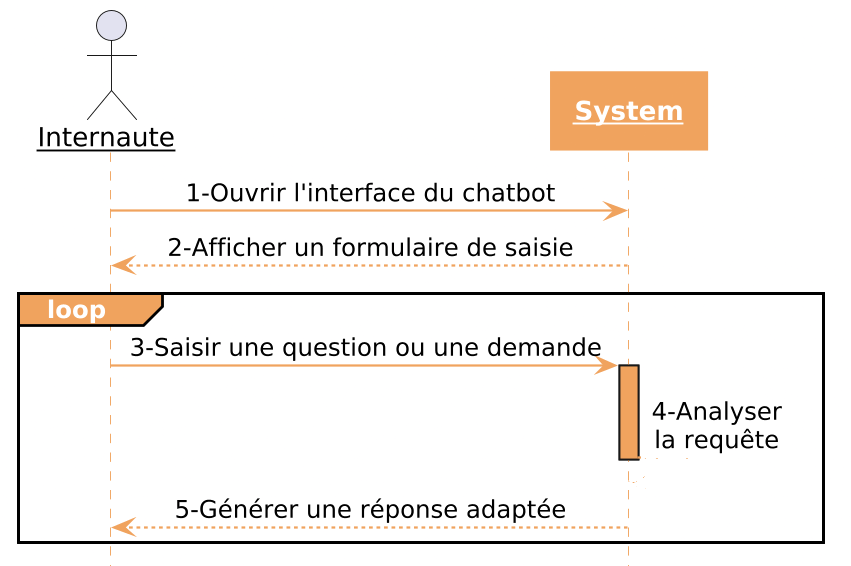
\includegraphics[width=0.7\textwidth]{Chapitres/Figures/Diag_seq_chatbot.png}
    \caption{Diagramme de séquence système de cas d'utilisation «Interagir avec Chatbot»}
    \label{fig:chatbot}
\end{figure}

%==========================================================
\section{Analyse des cas d'utilisation de l'acteur "Utilisateur''}
\label{sec:acteur_utilisateur_s2}

\subsection{Analyse de cas d'utilisation "Voir score client''}
\label{sec:voir_score}

La section suivante présente l'analyse du cas d'utilisation "Voir score client''
de l'acteur utilisateur.

\begin{table}[H]
\centering
\caption{Description textuelle du cas d'utilisation "Voir score client''}
\label{tab:voir_score}
\renewcommand{\arraystretch}{1.35}
\begin{tabular}{|p{3.5cm}|p{10cm}|}
\hline
\textbf{Élément} & \textbf{Description} \\
\hline
Nom & Voir score client \\
\hline
Acteur & Utilisateur \\
\hline
Description brève & Permet à l'utilisateur de consulter le score de fiabilité calculé automatiquement à partir de son historique de location. \\
\hline
Précondition & L'utilisateur est authentifié. \newline
               Le système est accessible. \\
\hline
Postcondition & Le score de fiabilité de l'utilisateur est affiché ainsi que les critères ayant contribué à son calcul. \\
\hline
Enchaînement principal &
1. L'utilisateur accède à son espace personnel. \newline
2. Le système calcule le score à partir de l'historique (retards, annulations, incidents). \newline
3. Le système affiche le score de fiabilité ainsi que son détail. \\
\hline
\textbf{Scénario alternatif} &
2.1 Historique insuffisant pour calculer un score. \newline
\quad 2.1.1 Le système affiche un score par défaut "100''. \newline
2.2 Erreur de calcul. \newline
\quad 2.2.1 Le système affiche un message d'erreur. \\
\hline
\end{tabular}
\end{table}

\begin{figure}[H]
    \centering
    
\includegraphics[width=0.7\textwidth]{Chapitres/figures/diag_seq_voir_score_client.png}
    \caption{Diagramme de séquence système de cas d'utilisation "Voir score client''}
    \label{fig:seq_voir_score}
\end{figure}


\section{Analyse des cas d'utilisation de l'acteur "Client''}
\label{sec:acteur_client_s2}

%----------------------------------------------------------
\subsection{Analyse de cas d'utilisation "Effectuer réservation''}
\label{sec:effectuer_reservation}

Afin de mieux illustrer le déroulement du scénario, nous proposons ci-après une
description textuelle accompagnée du diagramme de séquence du cas d'utilisation
"\textbf{Effectuer réservation}''.

\begin{table}[H]
\centering
\caption{Description textuelle du cas d'utilisation "Effectuer réservation''}
\label{tab:effectuer_reservation}
\renewcommand{\arraystretch}{1.35}
\begin{tabular}{|p{3.5cm}|p{10cm}|}
\hline
\textbf{Élément} & \textbf{Description} \\
\hline
Nom & Effectuer réservation \\
\hline
Acteur & Client \\
\hline
Description brève & Permet au client de réserver une voiture disponible pour une période déterminée. \\
\hline
Précondition & Le client est authentifié. \newline
               Le système est accessible. \newline
               Au moins un véhicule est disponible. \\
\hline
Postcondition & La réservation est enregistrée et son statut est "~En attente~''. \newline
                Le client reçoit une confirmation de sa demande. \\
\hline
Enchaînement principal &
1. Le client choisit une voiture à réserver.\newline
2. Le système affiche les détails de la voiture.\newline
3. Le client demande une réservation.\newline
4. Le système affiche le formulaire de saisie des informations de réservation.\newline
5. Le client saisit les informations de réservation (date, jours).\newline
6. Le système vérifie les informations saisies.\newline
7. Le système vérifie la disponibilité de la voiture.\newline
8. Le système affiche un message de confirmation de réservation.\\
\hline
\textbf{Scénario alternatif} &
6.1 Champs incomplets.\newline
\quad 6.1.1 Le système affiche un message d'erreur.\newline
7.1 Voiture indisponible.\newline
\quad 7.1.1 Le système affiche le message « La voiture est réservée pour la date saisie ».\\
\hline
\end{tabular}
\end{table}

\begin{figure}[H]
    \centering
    
\includegraphics[width=0.8\textwidth]{Chapitres/figures/Diag_seq_effectuer_reservation.png}
    \caption{Diagramme de séquence système de cas d'utilisation "Effectuer réservation''}
    \label{fig:seq_effectuer_reservation}
\end{figure}

%----------------------------------------------------------
\newpage
\subsection{Analyse de cas d'utilisation "Consulter réservations en cours''}
\label{sec:consulter_reservations}

Afin de mieux illustrer le déroulement du scénario, nous proposons ci-après une
description textuelle accompagnée du diagramme de séquence du cas d'utilisation
"\textbf{Consulter réservations en cours}''.

\begin{table}[H]
\centering
\caption{Description textuelle du cas d'utilisation "Consulter réservations en cours''}
\label{tab:consulter_reservations}
\renewcommand{\arraystretch}{1.35}
\begin{tabular}{|p{3.5cm}|p{10cm}|}
\hline
\textbf{Élément} & \textbf{Description} \\
\hline
Nom & Consulter réservations en cours \\
\hline
Acteur & Client \\
\hline
Description brève & Permet au client de consulter l'état de ses réservations actives. \\
\hline
Précondition & Le client est authentifié. \newline
               Le système est accessible. \\
\hline
Postcondition & La liste des réservations en cours est affichée avec leur statut respectif. \\
\hline
Enchaînement principal &
1. Le client accède à la section "Mes réservations''. \newline
2. Le système récupère les réservations associées au compte client. \newline
3. Le système affiche la liste des réservations avec leur statut (En attente, Confirmée, En cours, Terminée). \newline
4. Le client sélectionne une réservation pour consulter les détails. \newline
5. Le système affiche les informations détaillées de la réservation. \\
\hline
\textbf{Scénario alternatif} &
Pas d'exceptions \\
\hline
\end{tabular}
\end{table}

\begin{figure}[H]
    \centering
    
\includegraphics[width=0.8\textwidth]{Chapitres/figures/diag_seq_consulter_reservations_en_cours.png}
    \caption{Diagramme de séquence système de cas d'utilisation "Consulter réservations en cours''}
    \label{fig:seq_consulter_reservations}
\end{figure}

%==========================================================
\section{Analyse des cas d'utilisation de l'acteur "Agence''}
\label{sec:acteur_agence_s2}

%----------------------------------------------------------
\subsection{Analyse de cas d'utilisation "Traiter réservations''}
\label{sec:traiter_reservations}

Pour mieux analyser le déroulement du scénario, nous proposons ci-après une description textuelle et un diagramme de séquence du cas
d'utilisation "\textbf{Traiter réservations}'' de l'acteur Agence.

\begin{table}[H]
\centering
\caption{Description textuelle du cas d'utilisation "Traiter réservations''}
\label{tab:traiter_reservations}
\renewcommand{\arraystretch}{1.35}
\begin{tabular}{|p{3.5cm}|p{10cm}|}
\hline
\textbf{Élément} & \textbf{Description} \\
\hline
Nom & Traiter réservations \\
\hline
Acteur & Agence \\
\hline
Description brève & Permet à l'agence de consulter, accepter ou refuser les demandes de réservation des clients. \\
\hline
Précondition & L'agence est authentifiée. \newline
               Des demandes de réservation existent dans le système. \\
\hline
Postcondition & La réservation est acceptée ou refusée. \newline
                Le statut de la réservation est mis à jour. \newline
                Le client est notifié de la décision. \\
\hline
Enchaînement principal &
1. L'agence consulte les demandes de réservations. \newline
2. Le système affiche la liste des demandes. \newline
3. L'agence sélectionne une demande. \newline
4. L'agence choisit d'accepter la réservation. \newline
5. Le système met à jour le statut de la réservation. \newline
6. Le système affiche un message "Réservation acceptée''. \newline
7. Le système envoie une notification d'acceptation au client. \\
\hline
\textbf{Scénario alternatif} &
4.1 Refus de la réservation. \newline
\quad 4.1.1 L'agence choisit de refuser la demande. \newline
\quad 4.1.2 Le système confirme le refus. \newline
\quad 4.1.3 Le système envoie une notification de refus au client. \\
\hline
\end{tabular}
\end{table}

\begin{figure}[H]
    \centering
    
\includegraphics[width=1\textwidth]{Chapitres/figures/seq_traiter_reservation.png}
    \caption{Diagramme de séquence système de cas d'utilisation "Traiter réservations''}
    \label{fig:seq_traiter_reservation}
\end{figure}

%----------------------------------------------------------
\subsection{Analyse de cas d'utilisation "Consulter statistiques-Agence''}
\label{sec:stats_agence}

Dans la suite, nous présentons une description textuelle accompagnée d'un diagramme
de séquence du cas d'utilisation "\textbf{Consulter statistiques}'' de l'acteur Agence.

\begin{table}[H]
\centering
\caption{Description textuelle du cas d'utilisation "Consulter statistiques-Agence''}
\label{tab:stats_agence}
\renewcommand{\arraystretch}{1.35}
\begin{tabular}{|p{3.5cm}|p{10cm}|}
\hline
\textbf{Élément} & \textbf{Description} \\
\hline
Nom & Consulter statistiques \\
\hline
Acteur & Agence \\
\hline
Description brève & Permet à l'agence de visualiser ses indicateurs de performance à travers un tableau de bord interactif. \\
\hline
Précondition & L'agence est authentifiée. \newline
               Le système est accessible. \\
\hline
Postcondition & Les indicateurs de performance sont affichés (nombre de réservations, taux d'occupation, chiffre d'affaires, satisfaction client). \\
\hline
Enchaînement principal &
1. L'agence accède à "~Statistiques~''. \newline
2. Le système collecte les données relatives à l'activité de l'agence. \newline
3. Le système génère et affiche les indicateurs clés (graphiques, tableaux, synthèses). \newline
4. L'agence consulte et analyse les données. \\
\hline
\textbf{Scénario alternatif} &
Pas d'exceptions \\
\hline
\end{tabular}
\end{table}

\begin{figure}[H]
    \centering
    
\includegraphics[width=1\textwidth]{Chapitres/figures/seq_stats_agence.png}
    \caption{Diagramme de séquence système de cas d'utilisation "Consulter statistiques-Agence''}
    \label{fig:seq_stats_agence}
\end{figure}

%==========================================================
\section{Analyse des cas d'utilisation de l'acteur "Administrateur''}
\label{sec:acteur_admin_s2}

%----------------------------------------------------------

%----------------------------------------------------------
\subsection{Analyse de cas d'utilisation "Consulter statistiques-Administrateur''}
\label{sec:stats_admin}

Dans la suite, nous présentons une description textuelle accompagnée d'un diagramme
de séquence du cas d'utilisation "\textbf{Consulter statistiques globales}'' de
l'acteur Administrateur.

\begin{table}[H]
\centering
\caption{Description textuelle du cas d'utilisation "Consulter statistiques-Administrateur''}
\label{tab:stats_admin}
\renewcommand{\arraystretch}{1.35}
\begin{tabular}{|p{3.5cm}|p{10cm}|}
\hline
\textbf{Élément} & \textbf{Description} \\
\hline
Nom & Consulter statistiques globales \\
\hline
Acteur & Administrateur \\
\hline
Description brève & Permet à l'administrateur de visualiser les indicateurs de performance globaux de l'ensemble de la plateforme afin de détecter les anomalies et d'améliorer le système. \\
\hline
Précondition & L'administrateur est authentifié. \newline
               Le système est accessible. \\
\hline
Postcondition & Les indicateurs globaux sont affichés (nombre total d'agences, de réservations, de clients, score moyen, anomalies détectées). \\
\hline
Enchaînement principal &
1. L'administrateur accède à"~Statistiques~''. \newline
2. Le système collecte les données globales de toutes les agences. \newline
3. Le système génère et affiche les indicateurs clés de performance (KPI). \newline
4. L'administrateur consulte les données. \newline
5. L'administrateur peut filtrer les données par période ou par agence. \\
\hline
\textbf{Scénario alternatif} &
Pas d'exceptions \\
\hline
\end{tabular}
\end{table}

\begin{figure}[H]
    \centering
    
\includegraphics[width=1\textwidth]{Chapitres/figures/seq_stats_admin.png}
    \caption{Diagramme de séquence système de cas d'utilisation "Consulter statistiques-Administrateur''}
    \label{fig:seq_stats_admin}
\end{figure}

%----------------------------------------------------------

\section{Diagramme de classe du deuxième sprint}
\label{sec:sec_diag_classe_sprint_2}

\begin{figure}[H]
    \centering
    
\includegraphics[width=1\textwidth]{Chapitres/figures/Diag_classe_sprint_2.png}
    \caption{Diagramme de classe du deuxième sprint}
    \label{fig:classe_sprint2}
\end{figure}

%==========================================================
\section{Conception des cas d'utilisation}
\label{sec:conception_s2}

Nous illustrerons dans cette section la conception de ce deuxième sprint à travers
la réalisation d'un diagramme des classes pour chaque module, ainsi que d'un
diagramme de séquence détaillé correspondant à chaque cas d'utilisation analysé.

%==========================================================
\subsection{Diagramme des classes participantes}
\label{sec:classes_participantes_s2}


\subsubsection{Diagramme des classes participantes par acteur "Utilisateur''}
\label{Diag_classes_participantes_utilisateur_s2}
\begin{figure}[H]
    \centering
    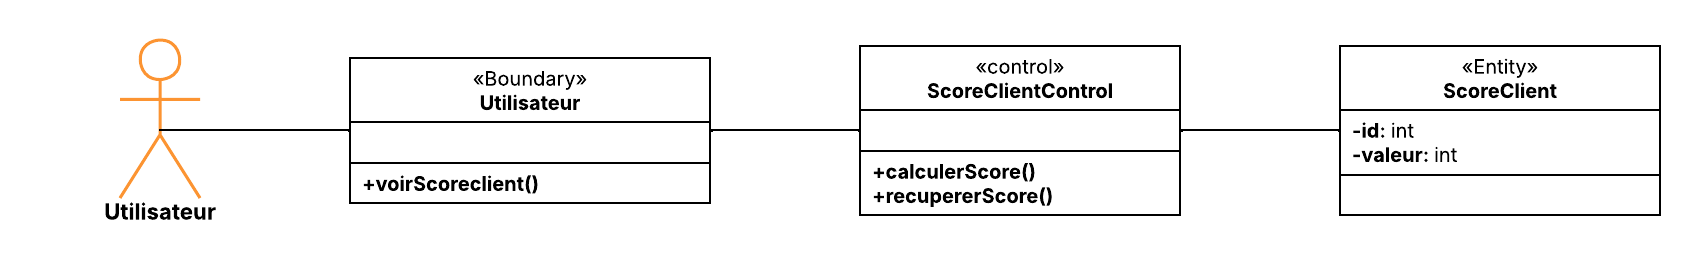
\includegraphics[width=1\textwidth]{Chapitres/Figures/classes_participantes__utilisateur_s2.png}
    \caption{Diagramme des classes participantes par acteur Utilisateur}
    \label{fig:classes_participantes_utilisateur_s2}
\end{figure}

\subsubsection{Diagramme des classes participantes par acteur "Client''}
\label{Diag_classes_participantes_client_s2}
\begin{figure}[H]
    \centering
    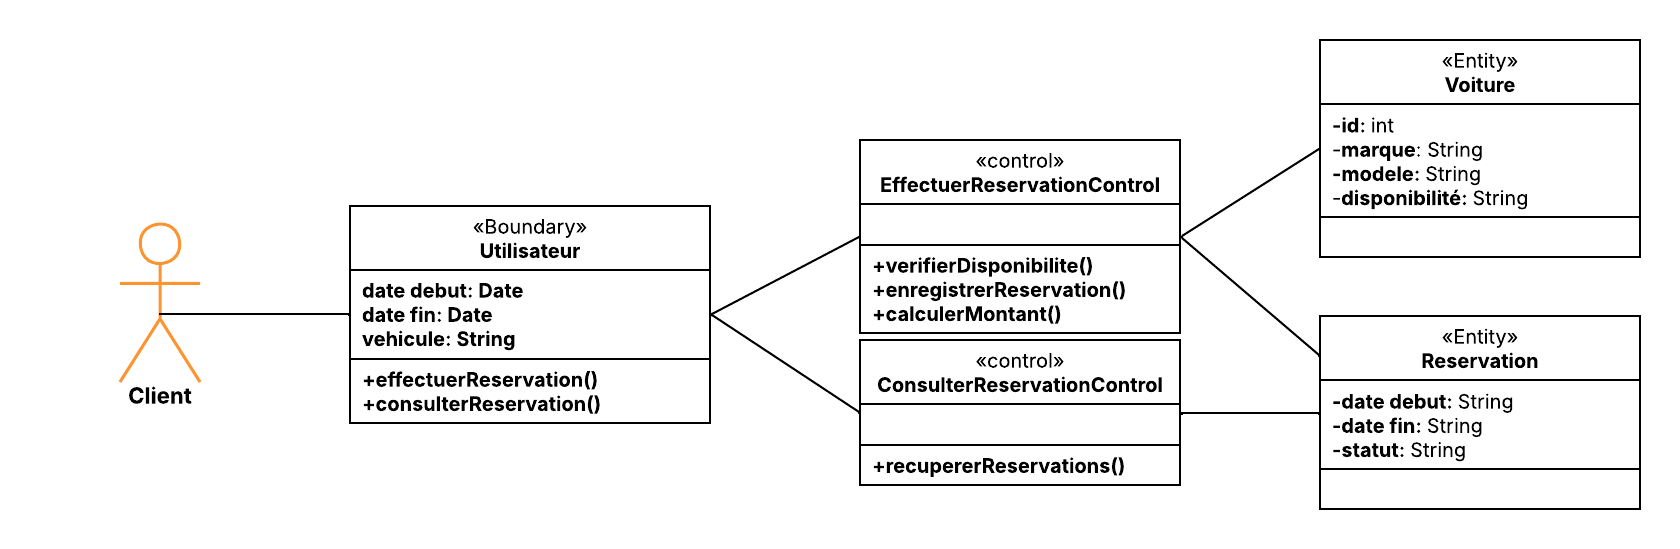
\includegraphics[width=1\textwidth]{Chapitres/Figures/classes_participantes__client_s2.png}
    \caption{Diagramme des classes participantes par acteur Client}
    \label{fig:classes_participantes_client_s2}
\end{figure}

\subsubsection{Diagramme des classes participantes par acteur "Agence''}
\label{Diag_classes_participantes_agence_s2}
\begin{figure}[H]
    \centering
    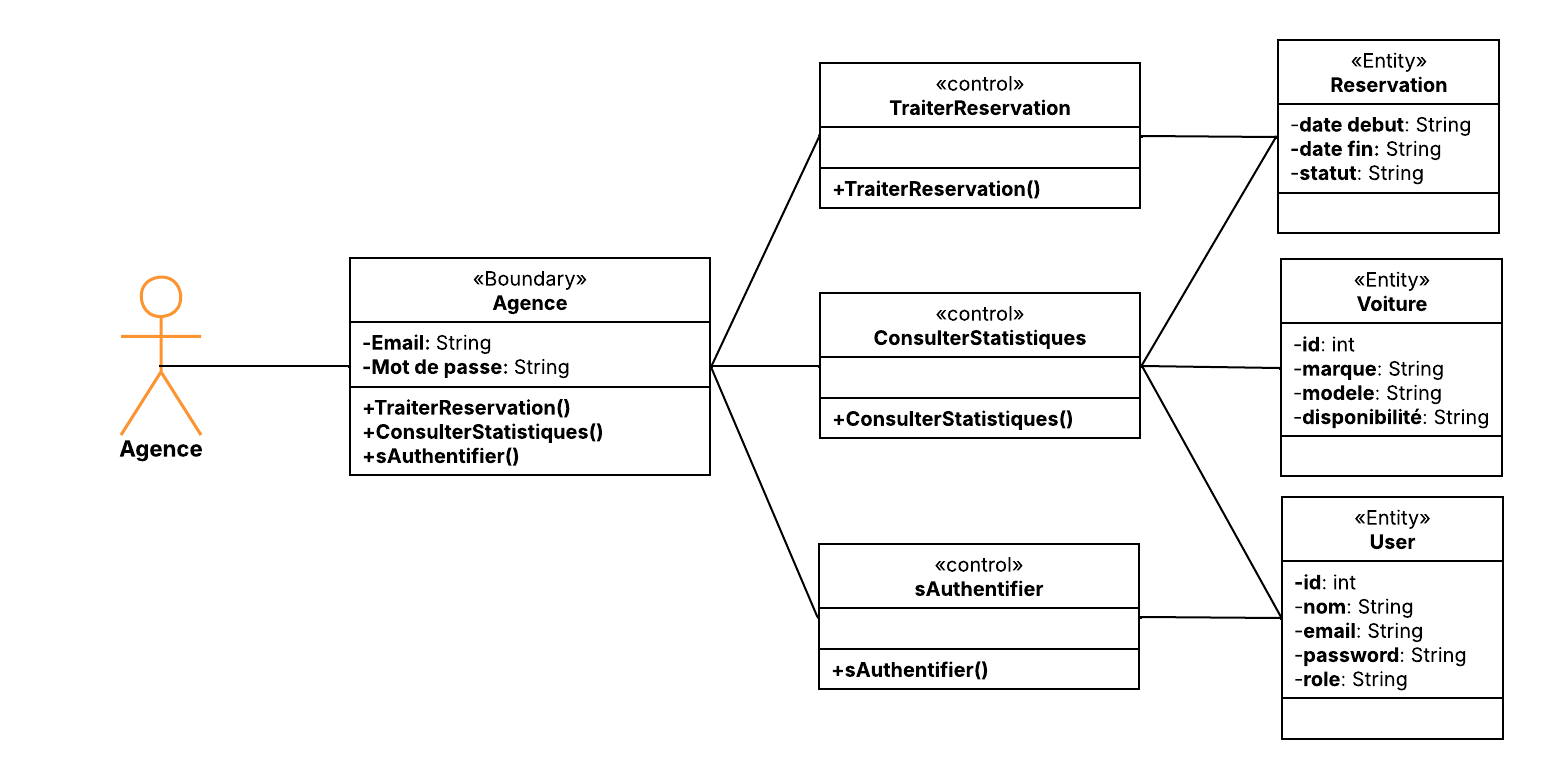
\includegraphics[width=1\textwidth]{Chapitres/Figures/classes_participantes__agence_s2.png}
    \caption{Diagramme des classes participantes par acteur Agence}
    \label{fig:classes_participantes_agence_s2}
\end{figure}

\subsubsection{Diagramme des classes participantes par acteur "Administrateur''}
\label{Diag_classes_participantes_administrateur_s2}
\begin{figure}[H]
    \centering
    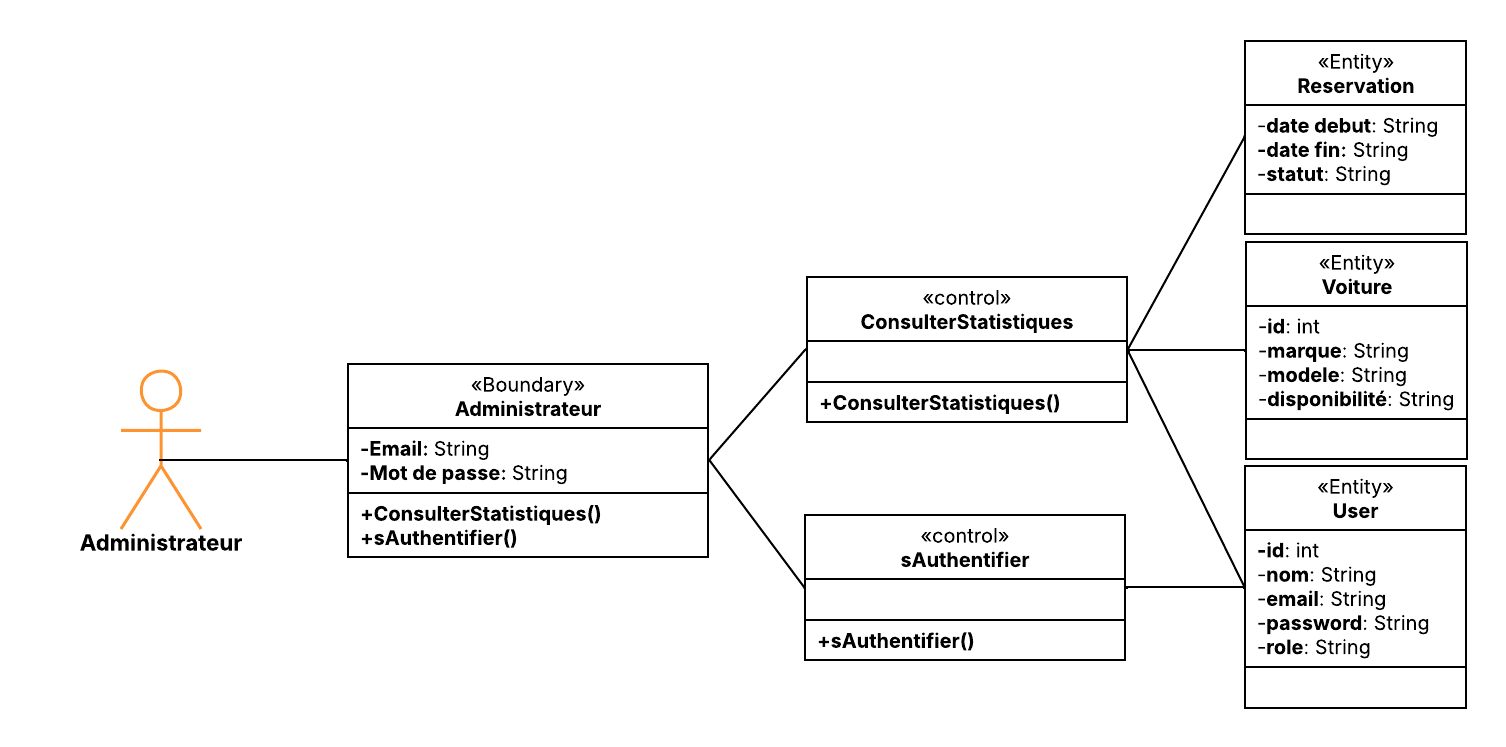
\includegraphics[width=1\textwidth]{Chapitres/Figures/classes_participantes__admin_s2.png}
    \caption{Diagramme des classes participantes par acteur Administrateur}
    \label{fig:classes_participantes_admin_s2}
\end{figure}
%%%%%%%%%%%%%%%%%%%%%%seq_détaillée%%%%%%%%%%%%%%%%%%%%%%%%%%%%%%%%%%%%%%%%%%%%%%%%%%%%%%%%%%%%%%%%%%%%%%%%%%%%%%%
\section{Diagrammes de séquence détaillés du deuxiéme sprint}
\label{sec:diag_seq_detail_s2}

%====================================================
\subsection{Diagrammes de séquence détaillés de l’acteur Utilisateur}
\label{sec:diag_seq_utilisateur_s2}

\subsubsection{Diagrammes de séquence détaillé du cas d’utilisation " Voir score client ''}
\label{sec:diag_seq_det_score_client}
\begin{figure}[H]
    \centering
    
\includegraphics[width=0.85\textwidth]{Chapitres/figures/diag_seq_det/seq_det_s2/seq_det_score_client.png}
    \caption{Diagramme de séquence détaillé du cas d’utilisation " Voir score client ''}
    \label{fig:seq_det_score_client}
\end{figure}

%====================================================
\subsection{Diagrammes de séquence détaillés de l’acteur Client}
\label{sec:diag_seq_client_s2}

\subsubsection{Diagrammes de séquence détaillé du cas d’utilisation " Effectuer réservation ''}
\label{sec:diag_seq_det_effectuer_reservation}
\begin{figure}[H]
    \centering
    
\includegraphics[width=0.95\textwidth]{Chapitres/figures/diag_seq_det/seq_det_s2/seq_det_effectuer_reservation.png}
    \caption{Diagramme de séquence détaillé du cas d’utilisation " Effectuer réservation ''}
    \label{fig:seq_det_effectuer_reservation}
\end{figure}

\subsubsection{Diagrammes de séquence détaillé du cas d’utilisation " Consulter reservation ''}
\label{sec:diag_seq_det_consulter_reservation}
\begin{figure}[H]
    \centering
    
\includegraphics[width=0.9\textwidth]{Chapitres/figures/diag_seq_det/seq_det_s2/seq_det_consulter_reservation.png}
    \caption{Diagramme de séquence détaillé du cas d’utilisation " Consulter réservations en cours ''}
    \label{fig:seq_det_consulter_reservation}
\end{figure}

%====================================================
\subsection{Diagrammes de séquence détaillés de l’acteur Agence}
\label{sec:diag_seq_agence_s2}

\subsubsection{Diagrammes de séquence détaillé du cas d’utilisation " Traiter réservations ''}
\label{sec:diag_seq_det_traiter_reservations}
\begin{figure}[H]
    \centering
    
\includegraphics[width=0.95\textwidth]{Chapitres/figures/diag_seq_det/seq_det_s2/seq_det_traiter_reservations.png}
    \caption{Diagramme de séquence détaillé du cas d’utilisation " Traiter réservations ''}
    \label{fig:seq_det_traiter_reservations}
\end{figure}

\subsubsection{Diagrammes de séquence détaillé du cas d’utilisation " Consulter statistiques agence ''}
\label{sec:diag_seq_det_Consulter_statistiques_agence}
\begin{figure}[H]
    \centering
    
\includegraphics[width=0.85\textwidth]{Chapitres/figures/diag_seq_det/seq_det_s2/seq_det_stat_agence.png}
    \caption{Diagramme de séquence détaillé du cas d’utilisation " Consulter statistiques agence ''}
    \label{fig:seq_det_stat_agence}
\end{figure}

%====================================================
\subsection{Diagrammes de séquence détaillés de l’acteur Administrateur}
\label{sec:diag_seq_admin_s2}

\subsubsection{Diagrammes de séquence détaillé du cas d’utilisation " Gérer messages ''}
\label{sec:diag_seq_det_gerer_message}
\begin{figure}[H]
    \centering
    
\includegraphics[width=0.9\textwidth]{Chapitres/figures/diag_seq_det/seq_det_s2/seq_det_gerer_messages.png}
    \caption{Diagramme de séquence détaillé du cas d’utilisation " Gérer messages ''}
    \label{fig:seq_det_gerer_messages}
\end{figure}

\subsubsection{Diagrammes de séquence détaillé du cas d’utilisation " Consulter statistiques administrateur ''}
\label{sec:diag_seq_det_stat_admin}
\begin{figure}[H]
    \centering
    
\includegraphics[width=0.85\textwidth]{Chapitres/figures/diag_seq_det/seq_det_s2/seq_det_stat_admin.png}
    \caption{Diagramme de séquence détaillé du cas d’utilisation " Consulter statistiques administrateur ''}
    \label{fig:seq_det_stat_admin}
\end{figure}
%%%%%%%%%%%%%%%%%%%%%%%%%%%%%%%%%%%%%%%%%%%%%%%%%%%%%%%%%%%%%%%%%%%%%%%%%%%%%%%%%%%%%%%%%%%%%%%%%%%%%%%%%%%%%%%%%%
%----------------------------------------------------------

\section{Diagramme de classe du deuxième sprint}
\label{sec:sec_diag_classe_sprint2}

\begin{figure}[H]
    \centering
    
\includegraphics[width=1\textwidth]{Chapitres/figures/Diag_classe_sprint_2.png}
    \caption{Diagramme de classe du deuxième sprint}
    \label{fig:diag_classe_sprint2}
\end{figure}

\section{Implémentation}
\label{sec:implementation_s2}

Le module d'implémentation du deuxième sprint présente la mise en œuvre technique des fonctionnalités développées, en détaillant leur réalisation au niveau du code et leur intégration dans l'application.

\subsection{Tables de la base de données}
\subsubsection{Tableau « reservations »}
\begin{table}[H]
\centering
\caption{Tableau « reservations »}
\label{tab:reservations}
\renewcommand{\arraystretch}{1.3}
\resizebox{\textwidth}{!}{%
\begin{tabular}{|l|l|p{4cm}|l|}
\hline
\textbf{Champs} & \textbf{Type} & \textbf{Libellé} & \textbf{Contraintes} \\
\hline
id & BigInt UNSIGNED & Identifiant unique de la réservation & PRIMARY KEY, AUTO\_INCREMENT, NOT NULL \\
\hline
user\_id & BigInt UNSIGNED & Identifiant du client & FOREIGN KEY (users), NOT NULL \\
\hline
vehicle\_id & BigInt UNSIGNED & Identifiant du véhicule & FOREIGN KEY (vehicles), NOT NULL \\
\hline
start\_date & Date & Date de début de location & NOT NULL \\
\hline
end\_date & Date & Date de fin de location & NOT NULL \\
\hline
pickup\_location & Varchar(255) & Lieu de récupération & NULLABLE \\
\hline
dropoff\_location & Varchar(255) & Lieu de retour & NULLABLE \\
\hline
base\_price & Decimal(10,2) & Coût base de location & NOT NULL \\
\hline
discount\_amount & Decimal(10,2) & Montant remise appliquée & NOT NULL, DEFAULT 0.00 \\
\hline
additional\_charges & Decimal(10,2) & Frais supplémentaires & NOT NULL, DEFAULT 0.00 \\
\hline
total\_price & Decimal(10,2) & Prix total à payer & NOT NULL \\
\hline
platform\_commission\_rate & Decimal(5,4) & Taux commission plateforme & NOT NULL, DEFAULT 0.0800 \\
\hline
platform\_commission & Decimal(10,2) & Commission plateforme & NOT NULL, DEFAULT 0.00 \\
\hline
agency\_payout & Decimal(10,2) & Paiement agence & NOT NULL, DEFAULT 0.00 \\
\hline
paid\_amount & Decimal(10,2) & Montant déjà payé & NOT NULL, DEFAULT 0.00 \\
\hline
remaining\_amount & Decimal(10,2) & Solde impayé & NOT NULL, DEFAULT 0.00 \\
\hline
\end{tabular}%
}
\end{table}


Le tableau suivant présente le dictionnaire des données du deuxième sprint, en précisant pour chaque table les attributs définis, leurs libellés ainsi que leurs types.

\subsubsection{Tableau « contact\_messages »}
\begin{table}[H]
\centering
\caption{Tableau « contact\_messages »}
\label{tab:contact_messages}
\renewcommand{\arraystretch}{1.3}
\resizebox{\textwidth}{!}{%
\begin{tabular}{|l|l|p{4cm}|l|}
\hline
\textbf{Champs} & \textbf{Type} & \textbf{Libellé} & \textbf{Contraintes} \\
\hline
id & BigInt UNSIGNED & Identifiant unique du message & PRIMARY KEY, AUTO\_INCREMENT, NOT NULL \\
\hline
name & Varchar(255) & Nom du contact & NOT NULL \\
\hline
email & Varchar(255) & Email du contact & NOT NULL \\
\hline
phone & Varchar(255) & Numéro téléphone & NULLABLE \\
\hline
subject & Varchar(255) & Sujet du message & NOT NULL \\
\hline
message & Text & Corps du message & NOT NULL \\
\hline
admin\_reply & Text & Réponse de l'admin (snapshot) & NULLABLE \\
\hline
replied\_by\_email & Varchar(255) & Email de l'admin qui répond & NULLABLE \\
\hline
replied\_at & Timestamp & Date de réponse & NULLABLE \\
\hline
is\_read & TinyInt(1) & Message lu & NOT NULL, DEFAULT 0 \\
\hline
submitted\_at & Timestamp & Date de soumission & NULLABLE \\
\hline
read\_at & Timestamp & Date de lecture & NULLABLE \\
\hline
created\_at & Timestamp & Date de création & NULLABLE \\
\hline
updated\_at & Timestamp & Date de modification & NULLABLE \\
\hline
\end{tabular}%
}
\end{table}

\subsubsection{Tableau « client\_reliability\_scores »}
\begin{table}[H]
\centering
\caption{Tableau « client\_reliability\_scores »}
\label{tab:client_reliability_scores}
\renewcommand{\arraystretch}{1.3}
\resizebox{\textwidth}{!}{%
\begin{tabular}{|l|l|p{4cm}|l|}
\hline
\textbf{Champs} & \textbf{Type} & \textbf{Libellé} & \textbf{Contraintes} \\
\hline
id & BigInt UNSIGNED & Identifiant unique du score & PRIMARY KEY, AUTO\_INCREMENT, NOT NULL \\
\hline
user\_id & BigInt UNSIGNED & Identifiant du client & FOREIGN KEY (users), NOT NULL \\
\hline
total\_reservations & Int & Nombre total de réservations & NOT NULL, DEFAULT 0 \\
\hline
completed\_reservations & Int & Réservations complétées & NOT NULL, DEFAULT 0 \\
\hline
cancelled\_reservations & Int & Réservations annulées & NOT NULL, DEFAULT 0 \\
\hline
late\_returns & Int & Retours en retard & NOT NULL, DEFAULT 0 \\
\hline
payment\_delays & Int & Retards de paiement & NOT NULL, DEFAULT 0 \\
\hline
damage\_incidents & Int & Incidents dommages & NOT NULL, DEFAULT 0 \\
\hline
total\_unpaid\_amount & Decimal(10,2) & Solde impayé total & NOT NULL, DEFAULT 0.00 \\
\hline
reliability\_score & Int & Score fiabilité (0-100) & NOT NULL, DEFAULT 100 \\
\hline
risk\_level & Enum('low','medium','high','blocked') & Niveau risque & NOT NULL, DEFAULT 'low' \\
\hline
admin\_notes & Text & Notes administrateur & NULLABLE \\
\hline
last\_calculated\_at & Timestamp & Dernière recalculation & NULLABLE \\
\hline
created\_at & Timestamp & Date de création & NULLABLE \\
\hline
updated\_at & Timestamp & Date de modification & NULLABLE \\
\hline
\end{tabular}%
}
\end{table}

\subsection{Réalisation des interfaces du deuxième sprint}

Nous présentons dans cette section les interfaces graphiques développées lors du deuxième sprint.


\subsubsection{Interface contact administrateur :}

\begin{figure}[H]
    \centering
    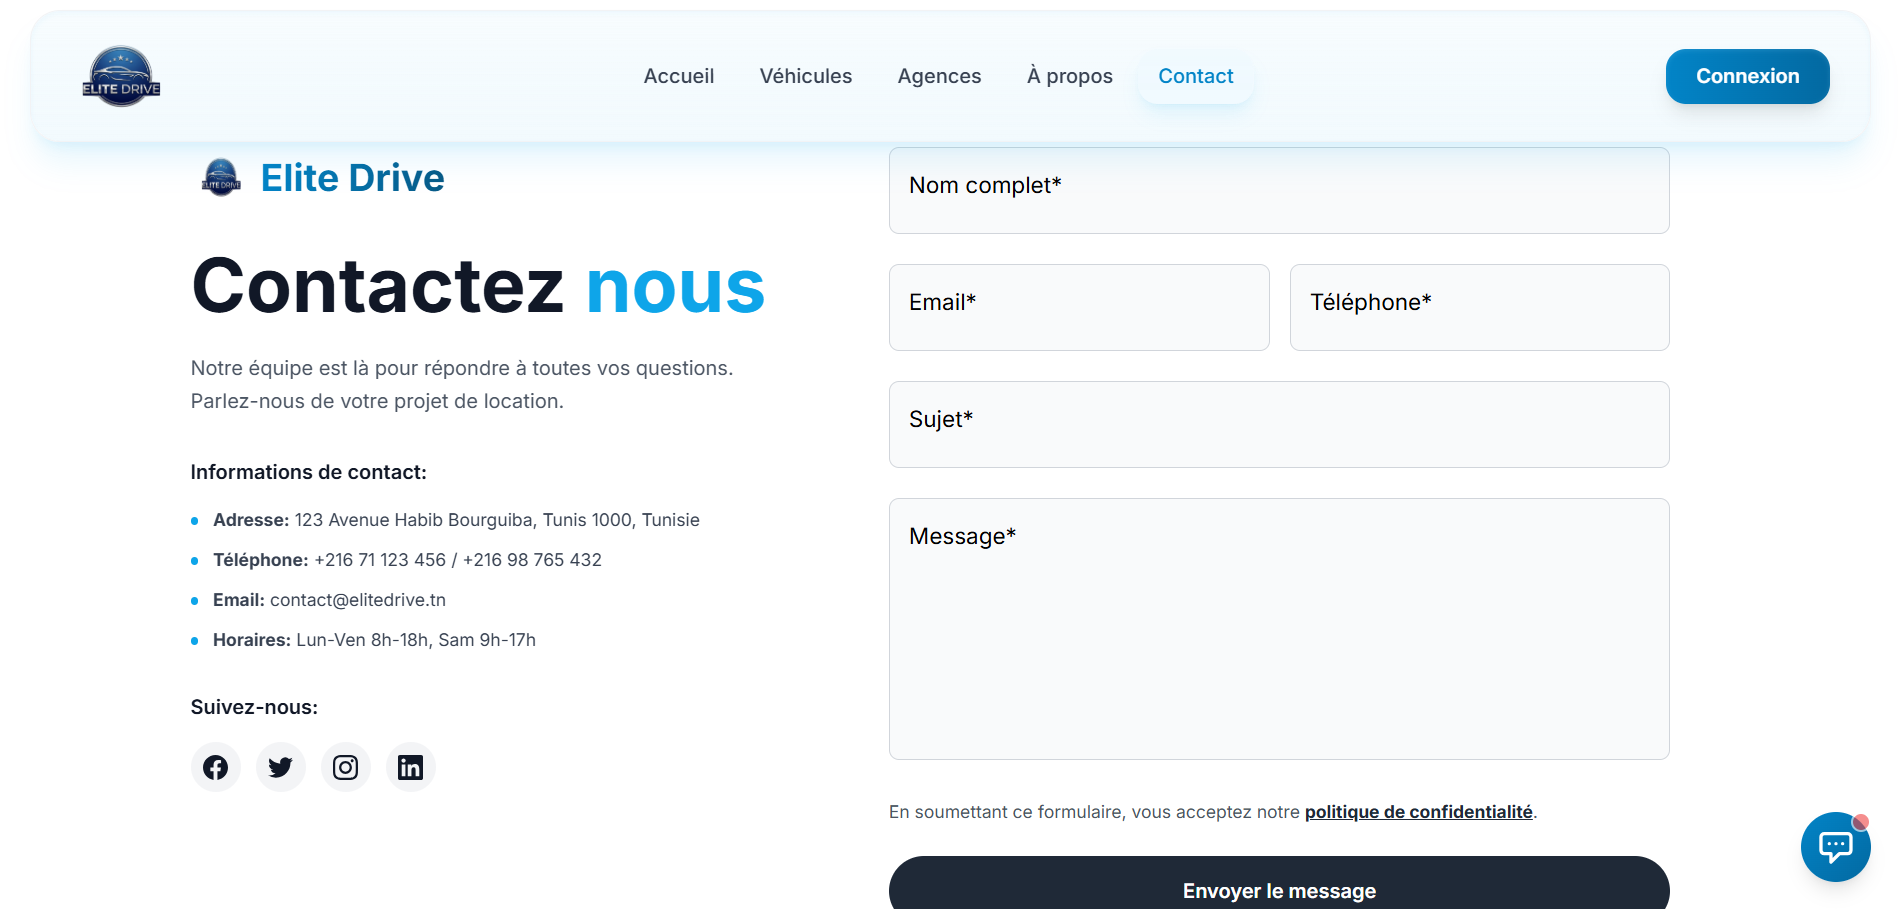
\includegraphics[width=0.9\linewidth]{Chapitres/Figures/inter_contact.png}    
    \caption{Interface contact administrateur}
    \label{fig:interface_contact_admin_s2}
\end{figure}


\subsubsection{Interface formulaire réservation :}

\begin{figure}[H]
    \centering
    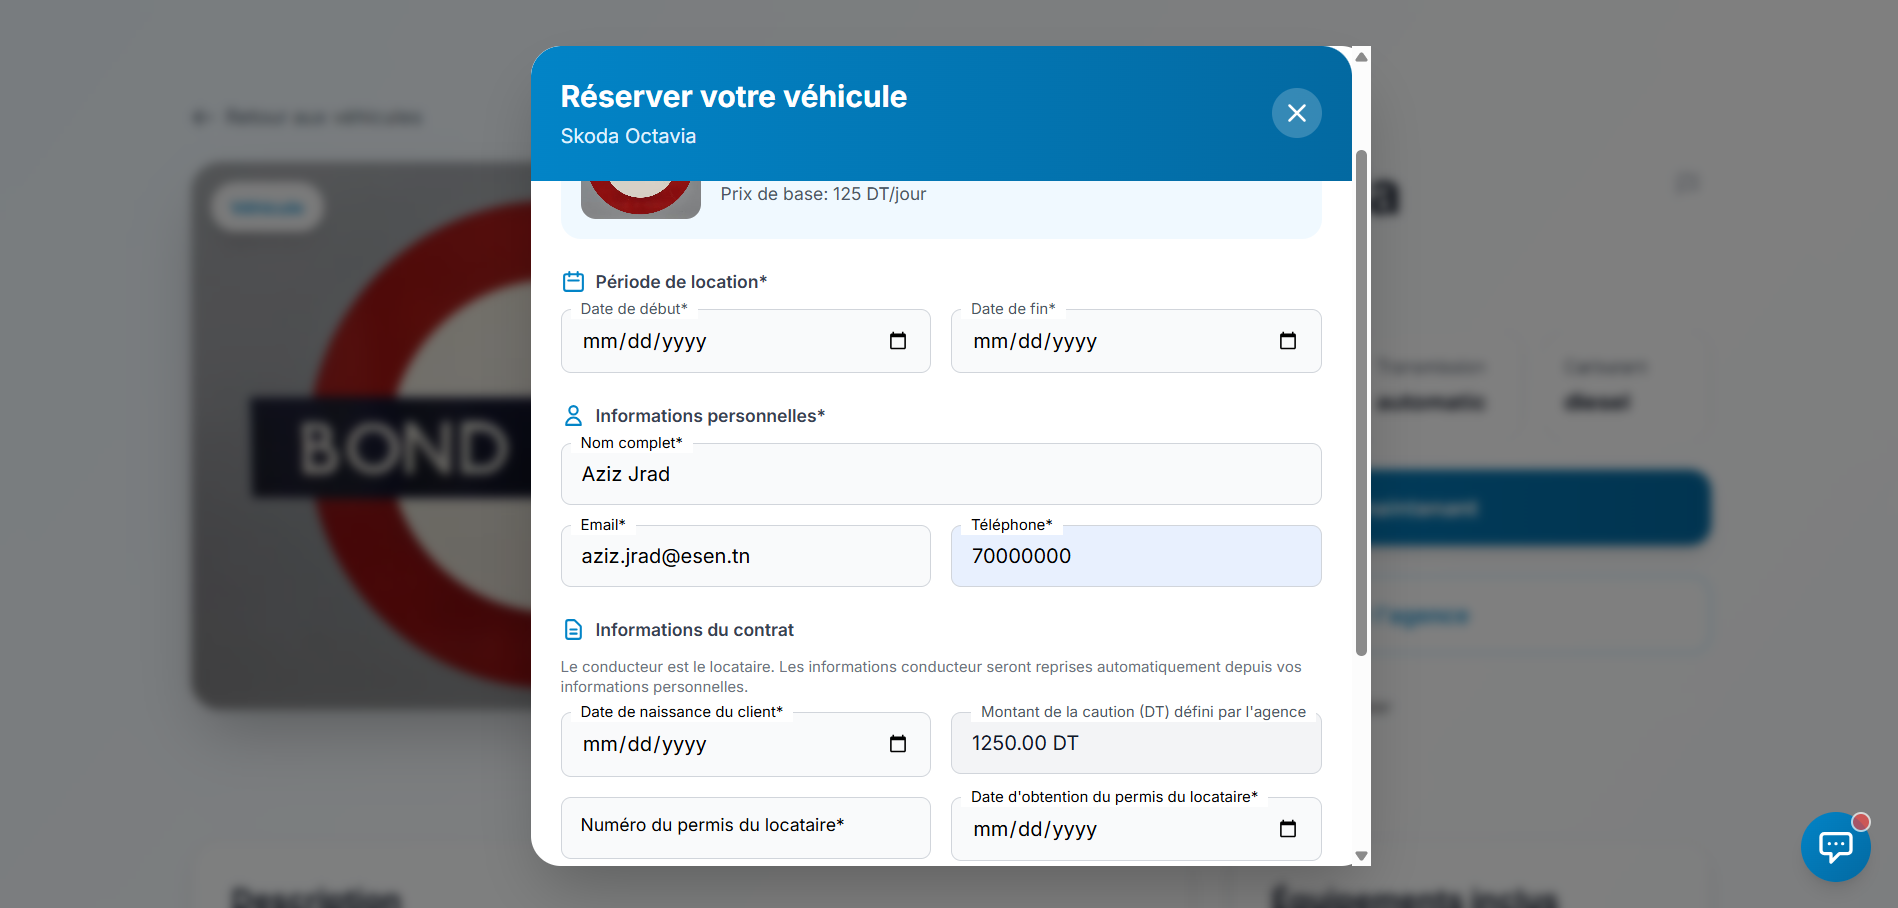
\includegraphics[width=0.9\linewidth]{Chapitres/Figures/inter_reservation.png}
    \caption{Interface réservation}
    \label{fig:interface_reservation_s2}
\end{figure}


\subsubsection{Interface statistiques globales :}

\begin{figure}[H]
    \centering
    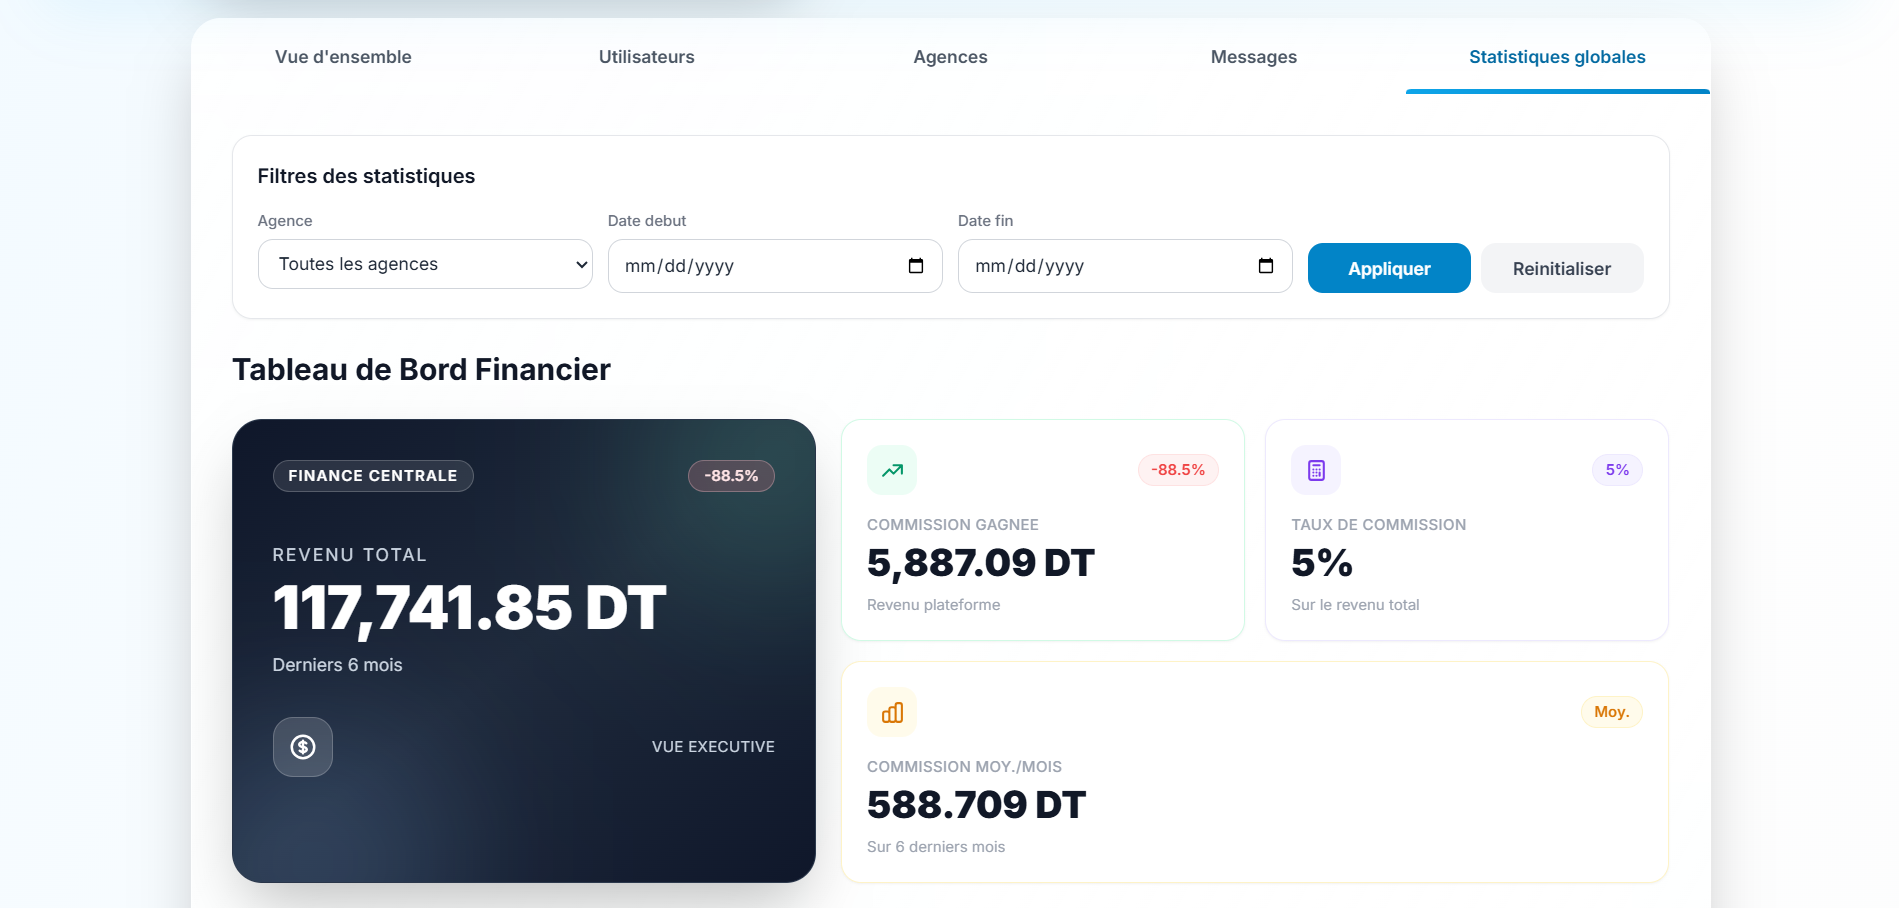
\includegraphics[width=0.9\linewidth]{Chapitres/Figures/inter_statsglobal.png}
    \caption{Interface statistiques globales}
    \label{fig:interface statistiques globales_s2}
\end{figure}



%----------------------------------------------------------
\section{Test}
\label{sec:test_sprint2}

\subsection{Test unitaire}
\label{sec:test_unitaire_s2}

\subsubsection{Test unitaire du cas d'utilisation "Voir score client''}

Cette section se concentre sur la reprise d'une partie du code pour le cas "Voir score client''.

\subsubsection*{--- Code source du cas d'utilisation "Voir score client''}

\begin{figure}[H]
    \centering
    
\includegraphics[width=0.9\textwidth]{Chapitres/figures/score_test.png}
    \caption{Test unitaire du cas d'utilisation "Voir score client''}
    \label{fig:test_unitaire_voir_score_client}
\end{figure}

%----------------------------------------------------------
\section{Conclusion}
\label{sec:conclusion_sprint2}

Dans le cadre de ce chapitre, nous avons mené le Sprint~2 selon une séquence logique
couvrant l'analyse des cas d'utilisation et la conception. Les fonctionnalités
développées — effectuer et suivre des réservations, visualiser le score de fiabilité,
traiter les réclamations, consulter les statistiques et gérer les messages — constituent
le cœur métier de la plateforme et assurent une expérience complète pour l'ensemble
des acteurs du système.

La phase suivante sera consacrée à la présentation des résultats obtenus, des
technologies utilisées, ainsi qu'au déploiement de la solution.

%%%%%%%%%%%%%%%%%%%%%%%%%%%%%%%%%%%%%%%%%%%%%%%%%%%%%%%%%%%%%%%%%%%%%%%%%%%
\chapter{Phase de clôture}
\label{Chapitre_5}
%%%%%%%%%%%%%%%%%%%%%%%%%%%%%%%%%%%%%%%%%%%%%%%%%%%%%%%%%%%%%%%%%%%%%%%%%%%
\section{Introduction}
\label{Introduction}
%%%%%%%%%%%%%%%%%%%%%%%%%%%%%%%%%%%%%%%%%%%%%%%%%%%%%%%%%%%%%%%%%%%%%%%%%%%
Ce chapitre présente la phase de clôture du projet, en mettant l'accent sur la finalisation
technique de la plateforme, les choix d'outils utilisés, ainsi que les résultats obtenus à l'issue
des deux sprints. L'objectif est de synthétiser le travail réalisé et de montrer la cohérence entre
les besoins définis au départ et la solution livrée.




%%%%%%%%%%%%%%%%%%%%%%%%%%%%%%%%%%%%%%%%%%%%%%%%%%%%%%%%%%%%%%%%%%%%%%%%%%%
\section{Environnement technique et outils adoptés}
\label{section5.2}
%%%%%%%%%%%%%%%%%%%%%%%%%%%%%%%%%%%%%%%%%%%%%%%%%%%%%%%%%%%%%%%%%%%%%%%%%%%
Pour concrétiser la plateforme web de gestion de location de véhicules, nous avons retenu
un ensemble d'outils permettant d'assurer la robustesse, la maintenabilité et l'évolutivité de
la solution.

\section{Technologies de développement}
Les technologies utilisées dans ce projet sont présentées dans le tableau suivant:

\begin{table}[!htbp]
\centering
\caption{Technologies utilisées}
\label{tab:technologies-utilisees}
\renewcommand{\arraystretch}{1.3}
\begin{tabular}{|l|p{10.2cm}|}
\hline
\textbf{Technologie} & \textbf{Description} \\
\hline

\includegraphics[height=0.7cm]{Chapitres/Figures/Laravel-Logo.png}\hspace{0.2cm}Laravel & Framework PHP utilisé pour développer le backend et exposer les API REST. \\
\hline

\includegraphics[height=0.7cm]{Chapitres/Figures/React-logo.png}\hspace{0.2cm}React & Bibliothèque utilisée pour construire l'interface utilisateur côté client. \\
\hline

\includegraphics[height=0.7cm]{Chapitres/Figures/Mysql-logo.png}\hspace{0.2cm}MySQL & Système de gestion de base de données relationnelle du projet. \\
\hline

\includegraphics[height=0.7cm]{Chapitres/Figures/vite-logo.png}\hspace{0.2cm}Vite & Outil de build et serveur de développement pour le frontend. \\
\hline

\includegraphics[height=0.7cm]{Chapitres/Figures/Tailwind-logo.png}\hspace{0.2cm}Tailwind CSS & Framework CSS utilitaire utilisé pour styliser rapidement l'interface. \\
\hline
\end{tabular}
\end{table}


%%%%%%%%%%%%%%%%%%%%%%%%%%%%%%%%%%%%%%%%%%%%%%%%%%%%%%%%%%%%%%%%%%%%%%%%%%%
\section{Logiciels utilisés}
\label{section5.3}
%%%%%%%%%%%%%%%%%%%%%%%%%%%%%%%%%%%%%%%%%%%%%%%%%%%%%%%%%%%%%%%%%%%%%%%%%%%
Les logiciels utilisés dans le cadre de ce projet sont présentés dans le tableau suivant:

\begin{table}[!htbp]
\centering
\caption{Logiciels utilisés}
\label{tab:logiciels-utilises}
\renewcommand{\arraystretch}{1.3}
\begin{tabular}{|l|p{10.2cm}|}
\hline
\textbf{Technologies} & \textbf{Description} \\
\hline

\includegraphics[height=0.7cm]{Chapitres/Figures/lucid-logo.png}\hspace{0.2cm}Lucidchart & Outil de modélisation UML utilisé pour les diagrammes de conception. \\
\hline

\includegraphics[height=0.7cm]{Chapitres/Figures/vscode-logo.png}\hspace{0.2cm}Visual Studio Code & Editeur de code utilisé pour le développement de l'application web. \\
\hline

\includegraphics[height=0.7cm]{Chapitres/Figures/overleaf-logo.png}\hspace{0.2cm}Overleaf (LaTeX) & Plateforme de rédaction utilisée pour la préparation du rapport. \\
\hline

\includegraphics[height=0.7cm]{Chapitres/Figures/teams-logo.png}\hspace{0.2cm}Microsoft Teams & Outil de visioconférence utilisé pour les réunions et les échanges à distance. \\
\hline

\includegraphics[height=0.7cm]{Chapitres/Figures/XAMPP-logo.png}\hspace{0.2cm}XAMPP & Environnement local regroupant Apache et PHP pour l'exécution et les tests de l'application. \\
\hline

\includegraphics[height=0.7cm]{Chapitres/Figures/phpmyadmin-logo.png}\hspace{0.2cm}phpMyAdmin & Interface web de gestion de la base de données MySQL. \\
\hline

\includegraphics[height=0.7cm]{Chapitres/Figures/github-logo.png}\hspace{0.2cm}Git/GitHub & Outils de gestion de versions et de collaboration sur le code source. \\
\hline
\end{tabular}
\end{table}




%%%%%%%%%%%%%%%%%%%%%%%%%%%%%%%%%%%%%%%%%%%%%%%%%%%%%%%%%%%%%%%%%%%%%%%%%%%
\section{Mise en production et organisation du déploiement}
\label{section5.4}
%%%%%%%%%%%%%%%%%%%%%%%%%%%%%%%%%%%%%%%%%%%%%%%%%%%%%%%%%%%%%%%%%%%%%%%%%%
La phase de déploiement a consisté à préparer une version stable de l'application,
incluant la configuration des variables d'environnement, la sécurisation des accès
et la vérification du bon fonctionnement des modules principaux.

Une attention particulière a été portée à:
\begin{itemize}
	\item la cohérence entre les environnements de développement et d'exécution,
	\item la fiabilité des échanges entre frontend et backend,
	\item la validation finale des fonctionnalités métier (réservation, réclamations,
	statistiques et messagerie).
\end{itemize}




	%%%%%%%%%%%%%%%%%%%%%%%%%%%%%%%%%%%%%%%%%%%%%%%%%%%%%%%%%%%%%%%%%%%%%%%%%%%
	\section{Choix technologiques}
	\label{sec:choix-technologiques}
	%%%%%%%%%%%%%%%%%%%%%%%%%%%%%%%%%%%%%%%%%%%%%%%%%%%%%%%%%%%%%%%%%%%%%%%%%%%

	\subsection{Architecture retenue dans notre projet}
	Dans notre application, nous avons adopté une architecture API Laravel (backend)
	+ SPA React (frontend). Le backend suit principalement une logique MVC enrichie
	par une couche Service, afin de séparer clairement les responsabilités et de
	faciliter la maintenance.

	\begin{itemize}
		\item \textbf{Modèle (Model)}: gère les entités métier et l'accès aux données
		(utilisateurs, agences, véhicules, réservations, paiements, etc.). Les modèles
		représentent la structure des données et les relations entre entités.

		\item \textbf{Contrôleur (Controller)}: reçoit les requêtes HTTP, orchestre le
		traitement et renvoie la réponse. Dans notre projet, les contrôleurs sont
		volontairement légers: ils délèguent la logique métier aux services et
		s'appuient sur une gestion centralisée des erreurs.

		\item \textbf{Vue}: dans une API REST, la « vue » est remplacée par des réponses
		JSON standardisées. Côté client, c'est l'interface React qui joue le rôle
		d'affichage et d'interaction utilisateur.
	\end{itemize}
	
\begin{figure}[H]
\centering
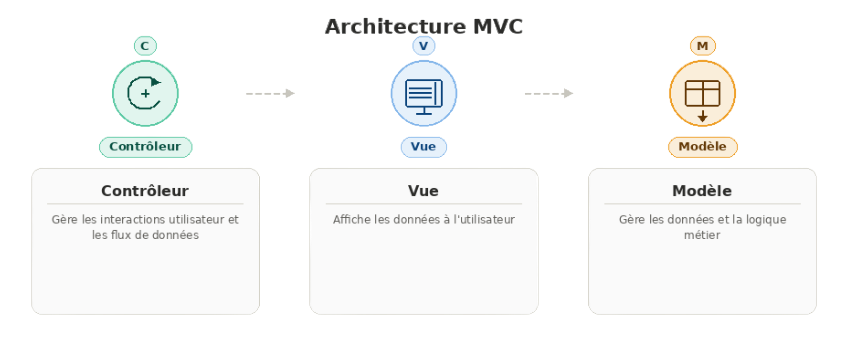
\includegraphics[width=0.9\textwidth]{Chapitres/Figures/diag_mvc.png}
\caption{Architecture MVC}
\label{fig:diag-mvc}
\end{figure}

\subsection{Diagramme de déploiement}
<<Un diagramme de déploiement fait partie de la catégorie des diagrammes structurels, car il décrit un aspect du système même. Dans le cas présent, le diagramme de
déploiement décrit le déploiement physique des informations générées par le logiciel sur
des composants matériels.>> \cite{lucidchart-deploiement}

\begin{figure}[H]
\centering
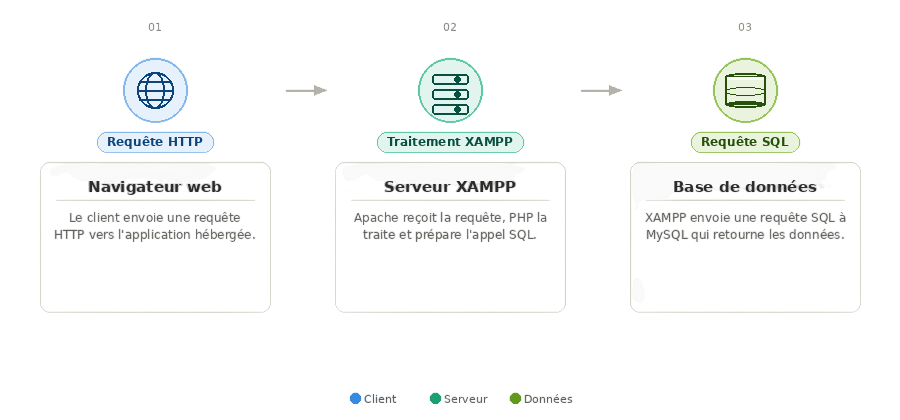
\includegraphics[width=0.95\textwidth]{Chapitres/Figures/diag_deploiement.png}
\caption{Diagramme de déploiement}
\label{fig:diag-deploiement}
\end{figure}

\subsection{Diagramme de Gantt}
Le diagramme de Gantt ci‑dessous récapitule les principales phases et tâches du projet, telles qu'elles ont été réalisées durant la période du 02/02/2026 au 15/05/2026.

\begin{table}[!htbp]
\centering
\caption{Diagramme de Gantt}
\label{tab:diagramme-gantt}
\renewcommand{\arraystretch}{1.3}
\resizebox{\textwidth}{!}{%
\begin{tabular}{|c|p{7.8cm}|c|c|c|}
\hline
\textbf{ID} & \textbf{Nom de tâches} & \textbf{Date début} & \textbf{Date fin} & \textbf{Durée} \\
\hline
1 & Auto-formation & 02/02/2026 & 12/02/2026 & 15 jours \\
\hline
2 & Étude et planification du projet & 13/02/2026 & 28/02/2026 & 17 jours \\
\hline
3 & Sprint 01 — Gérer des intervenants & 01/03/2026 & 21/03/2026 & 28 jours \\
\hline
4 & Sprint 02 — Gérer des processus des réservations & 01/04/2026 & 23/04/2026 & 29 jours \\
\hline
5 & Liaison et clôture & 01/05/2026 & 10/05/2026 & 10 jours \\
\hline
6 & Rédaction du rapport & 02/02/2026 & 11/05/2026 & 99 jours \\
\hline
\multicolumn{4}{|r|}{\textbf{Période couverte}} & \textbf{02/02/2026 -- 11/05/2026} \\
\hline
\end{tabular}%
}
\end{table}

\begin{figure}[H]
\centering
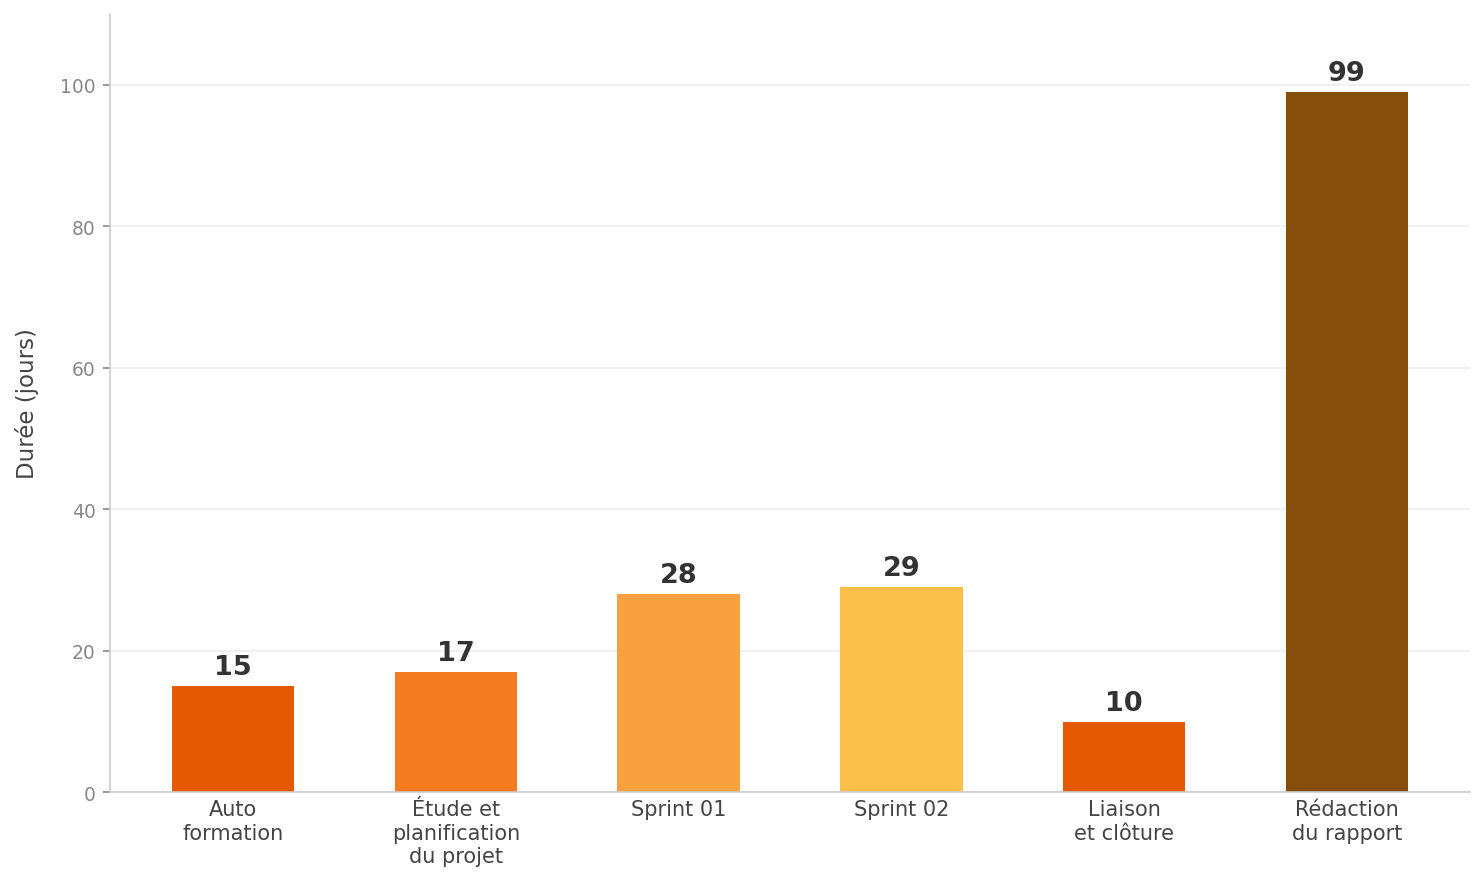
\includegraphics[width=0.95\textwidth]{Chapitres/Figures/gantt.png}
\caption{Diagramme de Gantt}
\label{fig:gantt-image}
\end{figure}

%%%%%%%%%%%%%%%%%%%%%%%%%%%%%%%%%%%%%%%%%%%%%%%%%%%%%%%%%%%%%%%%%%%%%%%%%%%
\section{Conclusion}
%%%%%%%%%%%%%%%%%%%%%%%%%%%%%%%%%%%%%%%%%%%%%%%%%%%%%%%%%%%%%%%%%%%%%%%%%%%
En conclusion, ce chapitre a permis de formaliser la phase finale du projet en présentant
les outils mobilisés, les choix techniques retenus et les résultats atteints. Cette étape confirme
la cohérence entre la planification initiale et la solution réalisée, tout en ouvrant la voie
à des améliorations futures de la plateforme.




%%%%%%%%%%%%%%%%%%%%%%%%%%%%%%%%%%%%%%%%%%%%%%%%%%%%%%%%%%%%%%%%%%%%%%%%%%%
\chapter*{Conclusion}
\addcontentsline{toc}{chapter}{Conclusion}
%%%%%%%%%%%%%%%%%%%%%%%%%%%%%%%%%%%%%%%%%%%%%%%%%%%%%%%%%%%%%%%%%%%%%%%%%%%

Ce rapport est le reflet de notre stage de fin d'études effectué au sein de
\textbf{Yes Internet}, dans le cadre de l'obtention de notre licence en
Informatique de Gestion à l'\textbf{École Supérieure de l'Économie Numérique (ESEN)}.

Durant cette période, nous avons eu l'opportunité de mettre en pratique nos acquis
académiques à travers le développement d'une plateforme web de gestion de
location de véhicules. L'objectif était de proposer une solution centralisée,
fiable et évolutive, capable de faciliter la gestion des agences, des
clients, des véhicules et des réservations.

<<<<<<< HEAD
Pour repondre aux exigences du projet, nous avons suivi une demarche structurée.
Nous avons d'abord realise une analyse de l'existant, puis identifie les
besoins fonctionnels et non fonctionnels des differents acteurs. Ensuite,
nous avons adopte la methodologie SCRUM afin de planifier et executer le
travail en iterations: construction du backlog produit, planification des
sprints, implementation progressive et validation des fonctionnalites.

Sur le plan technique, notre solution s'appuie sur les outils principaux suivants:
Laravel, React, MySQL, Tailwind CSS et
Vite. Nous avons egalement utilise Git/GitHub pour le versioning,
Lucidchart pour la modelisation, Visual Studio Code pour le
developpement et XAMPP pour l'environnement local. Ces choix nous ont
permis de maintenir une architecture claire, une bonne qualite de code et un suivi
rigoureux du projet.

Ce stage a ete tres enrichissant, car il nous a permis de renforcer nos competences
techniques et organisationnelles, notamment en conception, en
developpement web full stack, en tests et en gestion du
temps. En perspective, la plateforme peut etre amelioree par l'integration de
fonctionnalites complementaires, telles que des notifications en temps
reel, des tableaux de bord plus avances et des mecanismes de
supervision securisee, afin d'optimiser davantage l'experience utilisateur
et la performance globale du systeme.
=======
Pour répondre aux exigences du projet, nous avons suivi une démarche structurée.
Nous avons d'abord réalisé une analyse de l'existant, puis identifié les
besoins fonctionnels et non fonctionnels des différents acteurs. Ensuite,
nous avons adopté la méthodologie SCRUM afin de planifier et exécuter le
travail en itérations : construction du backlog produit, planification des
sprints, implémentation progressive et validation des fonctionnalités.
>>>>>>> cc5484eb8c9f96bd8d3b034b8b0e3a775f34df87

Sur le plan technique, notre solution s'appuie sur les outils suivants :
\textbf{Laravel} pour le développement de l'API REST et la gestion de la
logique métier, \textbf{React} pour la construction des interfaces utilisateur
sous forme de SPA, \textbf{MySQL} pour le stockage et la gestion des données
relationnelles, \textbf{Tailwind CSS} pour la mise en forme et le design des
composants, et \textbf{Vite} pour la compilation et l'optimisation du frontend.
Nous avons également utilisé \textbf{Git/GitHub} pour le versioning du code,
\textbf{Lucidchart} pour la modélisation UML, \textbf{Visual Studio Code} comme
environnement de développement et \textbf{XAMPP} pour l'environnement local.
Ces choix nous ont permis de maintenir une architecture claire, une bonne
qualité de code et un suivi rigoureux du projet.

Ce stage a été une expérience professionnelle formatrice, qui nous a permis de consolider nos compétences en développement web full stack et de contribuer concrètement à la transformation numérique d'une agence tunisienne spécialisée dans les solutions web. Il nous a également préparés à intégrer le monde professionnel en nous confrontant à des contraintes réelles : respect des délais, communication avec le client, prise de décision technique et travail en équipe. Cette expérience constitue ainsi un tremplin solide vers une carrière dans le développement logiciel et l'ingénierie des systèmes d'information.

En perspective, plusieurs axes d'amélioration peuvent être envisagés pour
faire évoluer la plateforme. L'intégration d'un gateway de paiement en ligne
permettrait de digitaliser complètement le processus de réservation. Le suivi
du comportement des clients offrirait une meilleure compréhension des habitudes
d'utilisation et renforcerait le système de scoring de fiabilité. Enfin, le
développement d'une application mobile élargirait l'accessibilité de la
plateforme et améliorerait l'expérience utilisateur au quotidien.



% Webographie placeholder
\chapter*{Webographie}
Cette section est gérée automatiquement par la commande \texttt{\textbackslash printbibliography[type=online, title=Webographie]} dans le fichier principal.\newline

% Les entrées web (type=online) sont déclarées dans le fichier \texttt{webographie.bib}.
% Fichier ajouté automatiquement pour éviter l'erreur d'\include.

\printbibliography[nottype=online, title=Bibliographie] % Pour la bibliographie
\printbibliography[type=online, title=Webographie] %Pour la webographie

\end{document}